 \documentclass[conference]{IEEEtran}
\IEEEoverridecommandlockouts
% The preceding line is only needed to identify funding in the first footnote. If that is unneeded, please comment it out.
\usepackage{cite}
% \usepackage{makecell}
\usepackage{hhline}
\usepackage{fancyhdr}
\usepackage[utf8]{inputenc}
\usepackage{amsmath,amssymb,amsfonts}
\usepackage{algorithmic}
\usepackage{graphicx}
\usepackage{textcomp}
\usepackage{blindtext}
\usepackage{pdfpages}
\usepackage{xcolor}
\usepackage{soul}
\usepackage{multirow}
\usepackage{booktabs}
\usepackage{array}
\usepackage{colortbl}
\usepackage{caption}
\usepackage{adjustbox}
\usepackage{url}
\usepackage{listings}
\sethlcolor{yellow}


\def\BibTeX{{\rm B\kern-.05em{\sc i\kern-.025em b}\kern-.08em
    T\kern-.1667em\lower.7ex\hbox{E}\kern-.125emX}}
\fancyhf{}
\pagenumbering{arabic}
\cfoot{"pagenumber"}
% set table of contents depth to include sections and subsections
\setcounter{tocdepth}{2}

\begin{document}
\begin{titlepage}
    \begin{center}
        \vspace*{7cm}
        {\fontsize{16}{20}\selectfont \textbf{Final Report}} \\ 
        \vspace{.6cm}
        {\fontsize{16}{20}\selectfont Design 2} \\ 
        \vspace{.6cm}
        % {\fontsize{12}{20}\selectfont Design 2 Project Midterm Review Report} \\
        % \vspace{.6cm}
        {\fontsize{16}{20}\selectfont Team 2: The Brain-Controlled Wheelchair} \\
        \vspace{.6cm}
        {\fontsize{12}{20}\selectfont Gerhort Alford (C00058921)} \\
        \vspace{.6cm}
        {\fontsize{12}{20}\selectfont Kaleb Guillot (C00405906)} \\
        \vspace{.6cm}
        {\fontsize{12}{20}\selectfont Samuel Whipp (C00240395)} \\
        \vspace{.6cm}
        \textit{\fontsize{12}{20}\selectfont November 22, 2023\\}
        \vfill
    \end{center}
\end{titlepage}
\thispagestyle{empty}
\pagestyle{empty}
\onecolumn
\tableofcontents
\twocolumn

\onecolumn
\clearpage
\thispagestyle{plain}
\pagestyle{plain}
\section*{\textbf{ABET Questions}}
\addcontentsline{toc}{section}{ABET Questions}
\begin{enumerate}
    \vspace{.6cm}
    
    \item \textit{How did this course provide you with an ability to identify, formulate, and solve complex engineering problems by applying principles of engineering, science, and mathematics?}
    \begin{itemize}
        \vspace{.3cm}
        \item Answer: This course gave us the ability to perform the scientific method for a problem that we have great interest in. We identified the problem, proposed a solution, performed research on related work, and are working to implement and experiment with the proposed solution. 
        \item Rank: 5
        \vspace{.3cm}
    \end{itemize}
    \item \textit{How did this course provide you with an ability to apply engineering design to produce solutions that meet specified needs with consideration of public health, safety, and welfare, as well as global, cultural, social, environmental, and economic factors?}
    \vspace{.3cm}
    \begin{itemize}
        \item Answer: With our design, there are many concerns to be addressed. These concerns not only include those addressed in the feasibility analysis, but also those which include safety of the user and a reliable and robust system. These problems have been weighed by the team, and solutions have been proposed through both software and hardware implementation. 
        \item Rank: 5
        \vspace{.3cm}
    \end{itemize}
    \item \textit{How did this course provide you with an ability to communicate effectively with a range of audiences?}
    \begin{itemize}
        \vspace{.3cm}
        \item Answer: This course provided the team with opportunities to present and communicate our ideas on a weekly basis to the class as well as to a wide range of audiences for E\&T Week.
        \item Rank: 5
        \vspace{.3cm}
    \end{itemize}
    \item \textit{How did this course provide you with an ability to recognize ethical and professional responsibilities in engineering situations and make informed judgments, which must consider the impact of engineering solutions in global, economic, environmental and societal contexts?}
    \begin{itemize}
        \vspace{.3cm}
        \item Answer: For a project aimed at assisting those less physically able, safety was the top priority. While this project aims at building a proof-of-concept, a product of similar nature must be reliable in all weather conditions and have protection from any malfunction or misuse.
        \item Rank: 4
        \vspace{.3cm}
    \end{itemize}
    \item \textit{ How did this course provide you with an ability to function effectively on a team whose members together provide leadership, create a collaborative and inclusive environment, establish goals, plan tasks, and meet objectives?}
    \begin{itemize}
        \vspace{.3cm}
        \item Answer: Through working on a team in which each member brought their own set of strengths and weaknesses, the work was able to be effectively delegated between them and the goals were able to be achieved.
        \item Rank: 4
        \vspace{.3cm}
    \end{itemize}
    \item \textit{ How did this course provide you with an ability to develop and conduct appropriate experimentation, analyze data and interpret data, and use engineering judgement to draw conclusions?}
    \begin{itemize}
        \vspace{.3cm}
        \item Answer: Through taking an in depth view of the project as a whole, and then systematically breaking that project down into sub-assemblies, sub-systems, and leaflets, each member of the team was able to develop their skills of interpreting appropriate experimentation
        \item Rank: 4
        \vspace{.3cm}
    \end{itemize}
    \item \textit{How did this course provide you with an ability to acquire and apply new knowledge as needed, using appropriate learning strategies?}
    \begin{itemize}
        \vspace{.3cm}
        \item Answer: The project was an entirely new forte for the team. It requires both members to reach out to peers and experts for advice as well as intensely research related subjects.
        \item Rank: 5
        \vspace{.3cm}
    \end{itemize}
\end{enumerate}
\twocolumn

    

\title{The Brain-Controlled Wheelchair{\footnotesize \textsuperscript{*}}
\thanks{This project was submitted for review on February 13, 2023. The project mentor and sponsor is Dr. Magdy Bayoumi. G.M. Alford is with the Electrical and Computer Engineering Department, University of Louisiana at Lafayette, LA 70504 USA (email: c00058921@louisiana.edu).\\K. J. Guillot is with the Electrical and Computer Engineering Department, University of Louisiana at Lafayette, LA 70504 USA (email: C00405906@louisiana.edu)}
}
\author{

\IEEEauthorblockN{Gerhort M. Alford, \textit{Student Member, IEEE}, Kaleb J. Guillot, \textit{Student Member, IEEE}, and Samuel Whipp}
% \IEEEauthorblockA{\textit{Member, IEEE} 
% \textit{}
% City, Country \\
% email address or ORCID
}

\maketitle
\thispagestyle{plain}
\pagestyle{plain}
\vspace{-7mm}

\begin{abstract}
This paper presents a proof of concept for an additional layer of control to a motorized wheelchair. This additional layer is through focused cognitive function, implemented as a BCI*. This system is implemented as an RC wheelchair, where a user can control an RC car through focused MI* while wearing an EEG* cap. Users train a machine learning model to recognize their EEG* waves while concentrating on specific motor functions. The trained model is then employed on live data to classify incoming signals and control the RC car. This project uses the Ultracortex Mark IV headset to retrieve EEG data and EEGNet to classify the data. The paper provides a comprehensive overview of the proposed design, including a timeline, potential safety concerns, and a cost analysis. The paper will explore alternatives to the design, including types of EEG headsets, signal processing hardware, and external sensors. The trade-offs associated with each alternative will be carefully considered and evaluated to determine the most viable option. This project will demonstrate the potential to improve mobility for those with physical limitations through use of non-invasive BCI. 
\end{abstract}

\begin{IEEEkeywords}
motor-imagery (MI), brain-computer interface (BCI), brain-machine interface (BMI), electroencephalogram (EEG), field programmable gate array (FPGA)
\end{IEEEkeywords}
\renewcommand{\thesubsection}{\Roman{section}.\Alph{subsection}}
\section{Introduction}
    The ability to move and live independently is a privilege that many take for granted. For millions of people around the world, physical limitations have made it challenging to operate a motorized wheelchair on their own. This leaves a significant number of people in need of further assistance from caregivers, decreasing feelings of independence and overall quality of life. Estimates indicate that between 1.4 and 2.1 million wheelchair users might benefit from a smart-powered wheelchair if it were able to provide a degree of additional assistance to the driver \cite{smart_wheelchairs}.  
    
    Impaired mobility has numerous downfalls. Psychologically, a decrease in independent mobility is associated to feelings of emotional loss, reduced self-esteem, isolation, stress, and fear of abandonment. In one's life, impaired mobility often decreases opportunities to socialize, resulting in social isolation, anxiety, and depression \cite{how_many_people}.
    
    Brain-Computer Interfaces (BCIs) are systems that allow the translation of real-time activity of the brain into commands that control devices. They rely solely on brain waves and can therefore provide a level of control for a device to a user suffering from a devastating neurodegenerative disorder \cite{noninvasive_brain}.

    In the last few years, BCI neurobiotic prototypes have flourished. Both invasive (implanted) and non-invasive (headset) approaches have produced devices such as robotic arms, exoskeletons, wheelchairs and telepresence robots \cite{learning_to_control}. In these devices, invasive BCI Systems much better signal to noise ratios due to the devices being implanted as close to the sources of the signals as possible. However, due to the portability, time constraints, and budget, electroencephalography (EEG) is a viable non-invasive option for this team's use. EEG uses electrodes placed at the scalp to retrieve brain signals, offering a view of multiple brain regions as well as high temporal resolution \cite{toward_brain_computer}.
    
    This paper proposes a solution for those unable to independently operate a motorized wheelchair - a brain-controlled wheelchair. This design utilizes a BCI system to translate real-time brain activity into commands that control the movement of a motorized wheelchair. This proposed model will work by using an EEG headset interfaced with a processing unit that will determine if the incoming signals dictate the movement of the wheelchair in a particular direction. To move, the processor will send signals to a motor controller that drives the movement of the electric motors. 
    
    To process the signals collected from the EEG cap, machine learning will be used to classify these signals into specific commands. There are six proposed categories of classification: forward, backward, left, right, stop, and none. The goal of the project is to process the signals locally, offloading the repetitive machine learning calculations to an onboard FPGA. However, for testing and verifying the model's effectiveness, the calculations will be offloaded to a remote server communicating with the onboard minicomputer via WiFi. 

    EEG signals themselves are not able to encapsulate the subtle movements that a wheelchair needs to accomplish. They can be decoded into commands like "forward," "backward," "left," and "right," but then the system is left to decide to what intensity to execute these commands. Does the user want to completely turn around or simply turn a few degrees? As the authors in \cite{learning_to_control} describe, the machine receiving the signals is akin to a passenger in a car giving a driver directions to a destination. The passenger does not need to tell the driver exactly how much force to apply to the accelerator and the brake; the driver is intelligent enough to make minute decisions. In the application of this project, the system requires a substantial amount of artificial intelligence to make context-based decisions. This will also help make the system safer to the user. Any error made while controlling the wheelchair, whether an accident from the user or a malfunction from the machine, may endanger the user. For these reasons, the system will be equipped with shared-control strategies. These are preventative measures instilled, such as sensors, lasers, or cameras, that will prevent collisions and regulate speed when approaching an object \cite{toward_brain_computer}. 
    
    Independent mobility increases opportunities in one's life, including educational and vocational \cite{how_many_people}. With the completion of this project, a step will be made in the direction of a more inclusive and well-rounded society.

\section{Related Work}
Brain-Controlled wheelchairs have been prevalent in research since the late 2000s. BCI wheelchairs fall into the larger category of smart wheelchairs (SWs), which are power wheelchairs (PWs) equipped with sensors, computers, and other assistive technologies \cite{a_comprehensive_review}. SWs have been under research since the middle of the 20th century, however, in recent years, the need for a device that accommodates a wider audience has remained while the research has unfortunately lost prevalence.  

    \subsection{Early Work}
    The development of PWs for individuals suffering from quadriplegia can be traced back to George Klein, who began his research following World War II. Prior to this time, individuals with quadriplegia were confined to their beds due to the limited technology available and were unable to lead fulfilling lives. In response to Klein's research, the American Wheelchair Company and Everest \& Jennings began producing PWs for mass distribution in 1956 \cite{a_comprehensive_review}. While these wheelchairs provided a degree of independence and improved the quality of life for many individuals with quadriplegia, they were not ideal for all patients and often required extensive safety modifications and improvements to increase comfort.

    Recognizing this issue, Dr. J. Leaman sought to create a more inclusive design for PWs in the late 1990s \cite{a_comprehensive_review}. At this time, many SWs were essentially mobile robots with attached seating, resulting in large form factors that made them impractical for everyday use. There were numerous types of input methods for these wheelchairs, including voice recognition, sight path detection, and computer vision \cite{smart_wheelchairs}. However, the primary drawback of these designs was the requirement for user supervision, as they did not accommodate individuals who were physically unable to control the chair through other means. For example, early SWs were only semi-autonomous, relying on user inputs such as a final destination or collision avoidance and leaving the navigation duties entirely up to manual input \cite{smart_wheelchairs}. 
    
    \subsection{Beginning of the Brain controlled wheelchair}
    Dr. Leaman finalized his invention in 2007, dubbed the iChair. This chair's movement was accomplished through a combination of a head tracking mouse and a Mount-n-Mover \cite{a_comprehensive_review}. In 2009, the authors of \cite{noninvasive_brain} took this a step further, using P300 neurophysiological protocol where the user would steer the wheelchair by concentrating on a certain section of the user interface. The advancement of this project was the use of computer vision. When the route for the wheelchair was selected by the user, the wheelchair would automatically drive to the destination. This took much of the mental strain involved out of the equation. Though, this system was not perfect; it suffered from the flaw of low information transfer rates, making instantaneous feedback impossible.  
    
    \subsection{Recent Years}
    In the past decade, there has been more attention towards developing reliable, noninvasive brain-controlled wheelchairs \cite{learning_to_control, self_paced, robotic_architecture, toward_brain_computer, biomedical-signal}. In 2012, the authors of \cite{self_paced} developed a system with a similar goal to this project, and with similar hardware. They employed the EMOTIV EPOC to gather brain signals and tasked the subject with performing motor-imagery (MI) tasks in order to steer the wheelchair. However, the headset was far too sensitive to noise and produced far too many false positives. In the following year, the authors of \cite{robotic_architecture} used a shared control architecture utilizing robotic perception and computer vision-based obstacle detection for an asynchronous approach to the concept. More recent projects have followed along with a shared control architecture, with the authors of \cite{learning_to_control} using integrated sensors to allow for external, computer based control to gather information about the surrounding environment to ensure user safety. This paper used a 32 channel ANT Neuro to compute a user's intent using the short-time direct directed transfer function (SdDTF). Other implementations took slightly different routes while still using similar technology. The authors of \cite{toward_brain_computer} used a virtual environment to test their implementation which involved a user focusing on one of many particular sensors connected to various parts of the user's body to move the wheelchair in a specific direction. 

    \subsection{Shared-Control Strategies}
    The broader category of brain-machine interfaces (BMI) employ hardware components and software protocols that protect both the user and the system itself. The components included in shared-control strategies take responsibility and strain away from the user and allow the system to handle the minute details. In \cite{robo-teleop}, mobile robots were controlled via EEG signals and protected with shared intelligence systems. These systems included software policies for obstacle-avoidance, measuring distance, accounting for user input, changes of direction, and a fusion of all four. The hardware employed included a laser range finder for obstacle detection and a 3-D camera. As one can imagine, this stragegy is very computationally intense, as this project required an embedded PC and onboard laptop.  

    In \cite{learning_to_control}, a brain-controlled wheelchair is employed and tested on participants affected with severe tetrapalegia. The term "mutual learning" is adopted to describe the closed loop control that improves brain signal modulation through feedback and their BMI decoder model that infers the underlying mental task from incoming brain signals after data-driven parameter estimation. Mutual learning allows the decoder to gain accuracy over time in both understanding the user's given command as well as interpreting the intended intensity behind the command. For example, if the decoder interprets that the user has been giving the command to turn left for some time, and the wheelchair is in a hallway where the only options to move are forward and backwards, then the decoder may decide that the user wishes to turn around. The authors of this paper incrementally re-calibrated the encoder based on the performance of the BMI. 

    \subsection{Machine Learning Strategies}
    To correctly classify incoming EEG signals, it is imperative to adequately employ a well documented and researched model. This model has to work accurately and reliably while remaining computationally inexpensive so as to characterize signals in a time efficient manner.  

    In recent years, one of the most common deep learning models has been the use of Long Short-Term Memory (LSTM) blocks. These blocks are implemented on EEG-Based signals for MI classification in \cite{lstm_eeg}. The authors first decompose the incoming signals into their respective frequency bands: alpha, beta, theta, and delta. The LSTM blocks are used as multi-class classifiers and combined with softmax layers for motion intention classification. This methodology displayed high accuracy, but was computationally intense. 

    A more simplistic network suitable for this project is the Convolutional Neural Network (CNN). The authors of \cite{deep_learning_eeg} compared five different deep learning models or EEG classification, with four of the five being CNNs. The experimenters measured the accuracy, training time, and inference time of each model while also comparing the effectiveness of each model from subject to subject. They concluded that EEGNet was, on average, the best performing, sporting a high accuracy and low inference time. However, they remarked that the inter-connectivity of the deep learning model varied heavily from subject to subject, remarking that different connective structures performed better or worse on select subjects. 

    EEGNet is designed to be computationally efficient, having fewer parameters than other deep learning models. It uses depth-wise separable convolutions to reduce the number of parameters while maintaining a high accuracy \cite{eegnet}. This model is promising for use of this project, as the model has been implemented on portable hardware in \cite{eegnet_processor_design}. This would be beneficial for an eventual FPGA implementation. 

    For improved accuracy in EEG-based motor imagery classification, the authors of \cite{dmtl_bci} propose an end-to-end learning strategy. The authors propose a novel model, named DMTL-BCI, wherin features are learned from raw signals automatically and the feature extractor and classifier are optimized simultaneously. Their proposal consists of three modules: the representation module, the reconstruction module, and the classification module. These modules are interconnected and share intermediate features, enhancing the generalization ability of the model and improving the performance of the classification with limited data. This is relevant to applications of this project, as the dataset for a given individual will be limited, and high accuracy is crucial for overall performance of the system. 
    

\section{Project Analysis}
    \subsection{Feasibility Analysis}\label{}

    %%%%%%%%%%%%%%%%%%%%%%%%%%%%%%%%%%%%%%%%%%%%%%%%
    From the team's research, multiple other projects have been found that have constructed a brain-controlled wheelchair using an EEG cap and have then used methods of either digital signal processing \cite{noninvasive_brain} or a combination of signal processing and machine learning to interpret the signal \cite{a_comprehensive_review, learning_to_control, robotic_architecture, toward_brain_computer}. The technological feasibility of this project will be divided into the different components that will be used to build the brain-controlled wheelchair and software. To control the motorized wheelchair, the planned component is an EEG cap from OpenBCI, the Ultracortex Mark IV Headset. This headset is responsible for sending raw EEG signal data to a minicomputer on the motorized wheelchair. The computational requirements for the minicomputer {is presently not known as the team has not yet reached a conclusion on the chosen machine learning model. The team may also take the alternative route of offloading the processing to a server. In this case, the onboard minicomputer would serve to collect, transmit, receive, and then output data.} Multiple models will be constructed and consequently trained on online data sets containing similar data to that of what is collected from the Ultracortex. These models will range from simple classification to the more complex, such as an RNN with LSTM blocks capturing temporal locality. After sufficient training and testing, the model will be selected. {If the team chooses to not offload the machine learning computations, a compromise will need to be reached between model accuracy and hardware capability.} 
    
    While the software model is being developed and tested, the group will work on data acquisition with the Ultracortex. This will work through subjects using motor imagery (MI) thoughts, where a user wearing the cap will focus on objects in their view and then concentrate on a particular direction to move said objects. The onboard processor will take the input of the EEG signals, and output signals to motor drivers connected to the motors controlling the wheels of the wheelchair. If time permits the machine learning model will be implemented using an FPGA for faster and more efficient processing. Translating a machine learning model to run on an FPGA, while not simple, is fully possible, as shown in \cite{fpga_intel}. Motorized wheelchairs are easily accessible and commercially available. In this project, the team plans to design their own motorized wheelchair; beginning with a standard manual wheelchair and then attaching motors and other necessary components. This motorized wheelchair will only be for testing purposes and will not be a final product. The main goal of mentor and sponsor Dr. Magdy  Bayoumi is to have the working machine learning model and hardware implementation done. From a technological perspective, this project is feasible.  
    %%%%%%%%%%%%%%%%%%%%%%%%%%%%%%%%%%%%%%%%%%%%%%%%
    
    % \subsection{Time Feasibility}
    The section of this project that is expected to be the most time-consuming will be handling and preprocessing the data. This task is delegated evenly between the two group members: Kaleb Guillot will code various machine learning models in python and use open source datasets to train the models to test for effectiveness. Both group members will then select a single model that balances effectiveness with complexity. Kaleb Guillot will then code the selected model in C, and then use toolkits to translate the model onto an FPGA. During this Gerhort Alford will work with the Ultracortex to perform data acquisition. Gerhort Alford will record EEG signals while performing MI tasks and will then preprocess the signals. This step will include noise filtration and feature selection and is expected to be very time-consuming. When Kaleb Guillot finishes coding a machine learning model in C, he will then move to assist Gerhort Alford with preprocessing the EEG signals from Gerhort Alford. Once the software implementation has been completed, the next step will be interfacing with the hardware of the motors. This task will primarily be handled by Gerhort Alford, however, assistance will be provided by Kaleb Guillot when needed. The length of time given for this project has been deemed feasible as project mentor and sponsor Dr. Bayoumi's main goal for us is to implement an effective machine learning model that decodes EEG signals. A Gantt Chart will be used to make sure progress is kept on time.
    
    
    % \subsection{Financial Feasibility}
    After compiling a list of parts required and speaking with project mentor and sponsor Dr. Magdy Bayoumi, the team has deemed this project financially feasible. Most of the components required for this project have already been obtained and most of the software required for this project has no cost. The raspberry pi 4, motor controllers, electric motors, and chair component costs are well within Kaleb Guillot's originally proposed budget of up to \$7,550, which has been approved by Dr. Bayoumi.  
    
    % \subsection{Legal Feasibility}
    The final consideration for the feasibility of this project is legal feasibility. The team plans on using noninvasive techniques of reading a user's brain signals so this project does not involve any medical procedure to take place on the user. Though wheelchairs do fall under Food and Drug Administration FDA and possibly Americans with Disabilities ACT ADA, in terms of this project, the goal is to build an initial prototype that can then be modified later to meet the requirements of the FDA and ADA. Guaranteeing reliable output and the safety of all users will be the main consideration when designing the final implementation. This test wheelchair will only be for initial testing not the final product. Legally, this project has been deemed feasible as the team will not be dealing with the aspect of the project that would require legal attention as this will mainly be the initial groundwork to be expanded upon later. 

    \subsection{Alternatives and Trade-offs}
    This project has been broken down into three sections: obtaining EEG signals, processing the signals, and translating the results into movement. The main consideration is the processor that will process the signals from the EEG cap. After discussion with the team, the likely option will be a Raspberry Pi 4 8GB model with the TUL Pynq Z2 FPGA as a signal processor. However, this is subject to change, as a working machine learning model must be chosen before choosing an adequate processor. The Raspberry Pi will serve to easily interface with the motor drivers, manual controls, and user displays. The FPGA will take on the task of the processing the signals from the EEG cap as it should be much faster at this task. Both these items are already on hand, so testing with them can begin as soon as the machine learning model is trained and team member Gerhort Alford has done research with the TUL Pynq Z2 FPGA.

    Another proposed option was to use the Raspberry Pi 4 8GB model with a Tensor processing unit. The Raspberry Pi will work as in the previous option with the FPGA but the Tensor processing unit will take on the task of processing the brain signals quickly. This option will be favored if the FPGA implementation of the machine learning model proves to be unrealistic due to hardware resource limitation and budget.  

    To acquire the signals, multiple EEG caps from multiple different companies have been considered. These companies are EMOTIV, OpenBCI, and G.Tec. EMOTIV creates headsets that are very easy to use and have eye-catching features. EMOTIV headsets are suitable for beginners to the field who only want to monitor EEG signals, performing well in areas such as psychology. These headsets are not suitable for engineering applications. To simply view the raw EEG signals, a special, expensive, yearly license is required. The EMOTIV headsets also have electrodes that are fixed in place, not allowing the experimenter to choose electrode placement through testing. OpenBCI headsets are designed with the engineering perspective in mind. They have fully open-source software and their hardware is highly configurable. Headsets can be taken apart, electrodes can be moved around, and raw data can be manipulated. This company makes it possible for the buyer to design their own headsets to support OpenBCI's electrodes using 3-D printing. G.Tec headsets take configuration to the next level, however the majority of this configuration is handled through preference selection on their website and then implemented by the company itself, rather than fully handled by the buyers as in the case of OpenBCI. These headsets are suitable for serious research projects, with the price tag reflecting their quality. G.Tec produces the headsets of choice of the authors of \cite{learning_to_control}, the inspiration for this project. After consideration, the group elected to use an Open BCI headset, specifically the Ultracortex Mark IV. This headset has both a reasonable price and a good reputation in the research community \cite{openbci-research}.
    
    When translating a brain signal into movement, there are several intermediate steps between decoding the EEG command and moving the wheelchair. An analogy can be made to giving directions to the driver of a car. When telling the driver where to go, general directions will be given such as "turn at the next light" or "make a u-turn." The driver will handle the minute movements of the car, e.g, applying the brake, or making sure that is is safe to make the u-turn. This same concept applies to a brain-controlled wheelchair. The user acts as the passenger, giving the wheelchair general directions. The wheelchair needs to decide for itself when and how to make the precise movements to allow for a same and smooth ride. These movements, sometimes referred to as computer vision, are made through processing sensor information about the environment surrounding the wheelchair. The sensors will be mounted on each of the four sides, allowing the wheelchair to gather a more complete picture and make an informed decision. The group has considered several different types of sensors, including ultrasonic, infrared, laser light (LIDAR), and cameras. Each provides its own set of pros and cons, but the group has opted for a combination of ultrasonic and infrared sensors due to their low cost and required processing power.  
    
    More details of alternative and trade-off analysis can be found in Appendix C. 

    \subsection{Preliminary Design}
    This section outlines the necessary components and their roles in the project. The responsibilities of the hardware and software are analyzed from the perspective of the component's functionality as well as their contribution to the system as a whole. Diagrams, flowcharts, and Failure Modes and Effects Analysis (FMEA) were used to analyze the project. More details of the preliminary design can be found in Appendix D. This section aims to provide a comprehensive overview of the design process and the steps taken to ensure that the final product meets the project's objectives.
    
    The Brain-Controlled Wheelchair involves using powerful hardware, an open-source EEG cap, and robust software to accomplish the design goal. The hardware chosen for this task includes an Orange Pi 5 16 GB RAM model, TUL Pynq Z2 FPGA, OpenBCI Ultracortex Mark IV EEG cap, two stepper motors, a stepper motor controller, two rotary photo encoders, ADS1115 16-bit analog-to-digital converter (ADC), a joystick, and the necessary components to implement a shared-control between the user and the wheelchair. The hardware used to implement computer vision includes a combination of infrared and ultrasonic sensors mounted at specified points on the wheelchair. To develop this project, coding will be done in Python and C/C++, using libraries from OpenBCI and Google to process data. Other software used for modeling includes Vivado and Onshape. When the FPGA is implemented to handle the repetitive calculations of the machine learning model, the code for the hardware will be written in Verilog.

    The project will begin by using the EEG cap to acquire a signal. The team will collaborate to build a dataset, pre-process the signals, and construct the machine learning model. Once the effectiveness of the model is verified, the onboard minicomputer will offload the repetitive parallel calculations to an FPGA. The output from the model will be used to command the motor controller. The team plans to conduct multiple testing phases, including using LEDs to monitor output, interfacing the headset with a miniature remote-controlled (RC) car, and finally, testing the proof-of-concept wheelchair. The team recognizes that building a complete motorized wheelchair for public use is outside of their scope of work. As a result, some common safety and quality of life features of normal motorized wheelchairs will be omitted. The team will still take the necessary precautions to ensure the safety of the user and those around the user during testing. 

    EEG signals will be read through the electrodes equipped on the Ultracortex Mark IV. The signals will transmit to a USB dongle via Bluetooth, which will be plugged into a USB 3.0 port of the Orange Pi 5. To control the wheelchair, a liquid crystal display (LCD) will show a virtual dot on an X-Y coordinate plane. The user will {imagine moving} the dot to a specific part of the screen. The movement of the dot will correspond to the movement of the wheelchair. The screen will also display helpful information to the user about the wheelchair's current movement, such as speed and direction. To acclimate the machine learning model to a given user, a training module will be designed for first-time users. The Orange Pi 5 will handle the initial pre-processing for the EEG signals as well as orchestrate the TUL Pynq Z2 FPGA, which will send and receive data at specified points of the machine learning model. 
    
    The wheelchair will be equipped with the safety precaution of a manual override joystick. {Including the joystick is beneficial for both testing and real-world use. During testing, while the headset and sensor commands are still being adjusted, the joystick will serve as an easy means for the testers to move the wheelchair. In real-world use, the inclusion of the joystick will be of use to those accompanying the wheelchair user. In the case of a fault or error in the system, another person will be able to safely move the wheelchair to the appropriate place.} The output of the joystick will always have priority over the output of the machine learning model. The joystick's directions will be interpreted using the ADS1115 16-bit ADC. The converter will communicate with the Orange Pi 5 via I2C. Based on output commands from either the EEG signals or the manual override joystick, the Orange Pi 5 will tell the motor drivers to start rotating the wheels in the desired direction. Distance sensors and position trackers will be used to give the system a better understanding of the surroundings and adjust the movement accordingly. 

    To accurately interpret the EEG signals from the Ultracortex Mark IV, there are several steps required. The team will begin with signal pre-processing to cleanse the signal. This will utilize helpful libraries provided by the manufacturer of the Ultracortex Mark IV: OpenBCI. Features will be extracted from the cleansed signal, and these features will serve as inputs to the machine learning model. The model will be orchestrated by the CPU on the Orange Pi 5, with the FPGA serving to relieve the Orange Pi of intensive repetitive calculations. A similar process will be taking place simultaneously with the data from the sensors. To make the movement of the wheelchair safe and smooth, the sensor data will also be processed and fed into a machine learning model of its own. This will give the wheelchair an idea of the surrounding environment and capture the minute movement that may be required to navigate safely. Separately, manual override controls will be developed using a joystick interfaced with the Orange Pi 5.

    \subsection{Final Design}
    The final design of the Brain-Controlled Wheelchair will consist of many of the components mentioned in the previous section of this report as well as new components that ensure the wheelchair operates safely and effectively. More details of the final design can be found in Appendix E. A list of components needed for the final design include the Ultracortex Mark IV EEG cap, an Orange Pi 5 minicomputer, the TUL Pynq Z2 FPGA, an override joystick, four ultrasonic and infrared sensors, an ADS1115 16-bit 4-channel analog-to-digital converter, two DC motors with worm drives, a DC motor controller, two photoelectric non absolute rotary encoders, a 10.5 inch LCD display, a 12V to 5V 50W buck converter, a 12V battery, a double male USB cable, and various other adapters and cables to wire the system together. 
    
    For initial testing and calibration, the design will be implemented on an RC car. Doing so ensures that the machine learning model's output is effective when interfaced with sensor data and the implemented computer vision operates seamlessly with the model's output. Each user that wishes to use the system will have an individualized profile consisting of their own specific EEG waves and trained model. The training of the profile will consist of a supervised learning method wherein the user will be prompted to move a virtual dot in a specified direction in the X-Y Cartesian plane on the LCD. The Ultracortex will monitor the incoming EEG signals and label them according to the prompted direction (forward, backward, left, right, stop, none). 

    The operation of this system will begin upon being powered on, wherein the system will undergo startup diagnostics to ensure all subsystems are functioning properly. Once the diagnostics complete, an overview of its performance will be displayed on the LCD and operation will begin. The Ultracortex will measure signals from its 16 electrodes, filter the signals with its onboard processor, and send the signals to the Orange Pi. Simultaneously, the Orange Pi will receive environmental data from the ultrasonic and infrared sensors as well as the inertial measurement unit (IMU). The environmental data will serve to implement a level of computer vision that will assist the wheelchair in capturing the precise movements to maneuver around obstacles and add a layer of safety for the user. The combined data will serve as input to the machine learning model on the Orange Pi. The Orange Pi will orchestrate the selected machine learning model, EEGNet \cite{eegnet}, a modified Convolutional Neural Network (CNN). Repetitive convolutions will be offloaded to the FPGA as done in \cite{eegnet_processor_design}. The output of the machine learning model will be sent back to the Orange Pi, wherein the environmental sensor data will be measured once more before the Orange Pi exports the output. The instructions on precisely how to maneuver the wheelchair will be processed on the Orange Pi and sent to the DC motor drivers. The motor drivers will transfer the signals to the DC worm drive motors. The photoelectric non-absolute rotary encoders and the IMU will send feedback about wheelchair movement to the Orange Pi. If the wheelchair is not moving properly, a software protocol will execute on the Orange Pi to correct the movement through the motor drivers. The system will be powered by a 12V battery with a 12V to 5V buck converter. The DC motors will run on 12V while the rest of the system will run on 5V.   

    The RC car used for initial testing and calibration will use an onboard Arduino wired to the environmental sensors and will communicate with the Orange Pi via NRF24L01 transceivers. The Orange Pi will be directly connected to both the Ultracortex and LCD. It will have the responsibility of not only communicating with the Arduino, but also with a remote server to transfer the input and output of the machine learning model.

    After analyzing the system's Failure Modes and Effects Analysis (FMEA) in table \ref{tab:fmea}, the team has made improvements. The first change is the switch from stepper motors to DC motors with worm drives. This prevents the wheelchair from moving in an uncontrollable manner in the situation of the system losing power. Additionally, the FMEA brought to light the importance of secure connections. To address this issue, the team plans to use cables which have specialized connectors and make custom cables when needed.

    Ubuntu is the operating system (OS) of choice for the Orange Pi 5. This OS has more online support and documentation compared to other Linux distributions and can safely run on the minicomputer. A modified version of RPi.GPIO called OPi.GPIO will be used for controlling the GPIO pins. OPi.GPIO is necessary due to the Orange Pi 5 having less GPIO pins but more communication IO pins than that of its counterpart, the Raspberry Pi. The developers of the Ultracortex, OpenBCI, have open source libraries available for obtaining and processing the EEG signals. Python will be the language of choice for processing the signals and implementing the machine learning model. Arduino-C++ will be used in the RC car implementation to obtain sensor data and communicate with the Orange Pi. 

    The hardware used in the system design is outlined in a level 2 functional block diagram in Appendix D Fig. \ref{fig:level-2} and in a schematic in Appendix E Fig. \ref{fig:schematic}. An upgrade is currently being considered to use the Orange Pi 5B which includes an embedded WiFi and Bluetooth module as well as a 256GB solid state drive. It is important to note that while the team works to implement the machine learning model on the FPGA, the computations will be offloaded to a remote server that will communicate with the Orange Pi via WiFi. 

\section{Experiments, Testing and Data Results}
To have an effective and thorough test of the entirety of the system, divisions were made in the components of the system into separate tests for subassemblies and subsystems. Experiments were designed independently and verified co-dependently. These tests were organized in a Comprehensive Modular Build and Testing Plan (P-CMBTP), with each subsystem containing component level tests to ensure a quality and relible build. The two subassemblies which encapsulate the scope of this project are the RC Wheelchair Subassembly and the Brain-Control Subassembly. 
    
    \subsection{Brain-Control Subassembly}
    This Subassembly encapsulates the entirety of the PC application. This includes not only the visual aspects of the application, but also the data processing and machine learning that happens underneath the hood. 

        \subsubsection{Headset Interface Subsystem}
        The Headset Interface Subsystem encapsulates the ability of the Ultracortex Mark IV to communicate with the PC. In the tests for the components of this subsystem, the Ultracortex Mark IV connects to the PC, sends data, writes data to a file, reads the data from the file, formats it, trains a model, and uses that model to generate predictions based on incoming data.  
        
        \subsubsection{EEG Interpretation Subsystem}
        The EEG Interpretation Subsystem is the most crucial component for steering the RC Wheelchair in the correct direction. One test to highlight, the Electrode placement test, was a point of trouble for the group. This test underwent many modifications, with the end result producing an incorrect output. This test was important due to the configurable nature of the Ultracortex Mark IV. In order to achieve accurate classifications from the EEG data, it is vital that the 16 electrodes that the group has at their disposal are those which are effectively able to measure distinctions in the data when a user imagines different motor imagery commands. Rather than use the results from this test, the group opted to use placements which are supported in relevant literature, namely \cite{method_of_electrode_selection, usable_out_of_box} .

    \subsection{RC Wheelchair}
    The section details a comprehensive evaluation of various components critical for the development of an EEG-controlled RC wheelchair. The testing encompassed motor drivers, DC motors, wheels, and the overall maneuverability of the wheelchair, with each test providing valuable insights into the system's performance and potential areas for improvement.

        \subsubsection{Motor Driver Test}
        In the motor driver test, the objective was to assess the functionality of the motor driver unit. Test procedures involved powering the system with specific voltage settings, evaluating duty cycles, and monitoring power consumption. A program was written to run on a Raspberry Pi Pico to control the motor driver and perform a three-stage test. Stage one would set the motor driver to drive the motors forward and increase the duty cycle. Stage two would do the same but in reverse. Stage three would rapidly spin the motors at maximum speed in one direction and then reverse direction. Stages one and two revealed the duty cycle at which the motors would begin to turn and the average power usage. Stage three showcased the worst-case power draw scenario. The data demonstrated that the motor driver performed as expected with no signs of overheating or device failure. Interestingly, it was observed that the issue related to uneven motor behavior during reverse maneuvering was likely rooted in the motors themselves, as the problem did not persist with the introduction of new motors. The unwanted behavior examined was that when in stage two reverse one motor would always start rotating earlier than the other. This finding confirmed the reliability of the motor driver.
    
        \subsubsection{Motor Test}
        The motor test focused on the DC motors' capacity to move the RC wheelchair and their thermal performance over an extended period. The data indicated that while the DC motors were capable of propelling the wheelchair, they exhibited strain, and the motors became notably warm to the touch after the test. This suggested that the motors were suited for short runs but could face overheating issues during extended usage. The root cause analysis revealed that the rubbing of the wheels against the body was a significant factor contributing to the motors' elevated temperature. To address this, the recommended modifications included replacing the DC motors with larger and higher-torque DC motors and upgrading the battery to a 12-volt system.
    
        \subsubsection{Wheel Test}
        The wheels test focused on assessing the quality and traction of the wheels used in the wheelchair. The data revealed significant slipping, indicating poor traction, and the wheels were noted to rub against the body, leading to instability. The interpretation indicated that the stiff rubber of the wheels was a primary cause of these issues. The recommended modification here was to design and 3D print new wheels using TPU rubber, known for better grip and maneuverability.
    
        \subsubsection{Maneuverability Test}
        The maneuverability test assessed the ease of controlling the RC wheelchair. Data showed unwanted turning during reverse movement, a concern linked to inconsistencies in motor behavior and wheel-body interaction. The recommended modifications included the construction of a new body for the RC wheelchair to address these root causes and improve overall maneuverability.

    \subsection{Noteworthy Test Results}

        \subsubsection{0.1.1.4 Straight Line and 0.1.1.5 90\textdegree Turn}
        To assess the RC wheelchair's capabilities in executing movement commands, particularly due to limitations in the machine learning model, only four movement commands—forward, a 90-degree left turn, a 90-degree right turn, and moving backward—are possible for demonstration purposes. The straight-line test and the 90-degree turn test were devised to evaluate the RC wheelchair's ability to execute these commands accurately. The RC wheelchair operates with five different command types: PS5 controller commands formatted as strings containing speed and direction controls for the left and right wheels, and four movement commands issued by the brain control system. The brain control system uses characters 'r' for forward movement, 'b' for backward movement, 'r' for a 90-degree right turn, and 'l' for a 90-degree left turn. Although the RC wheelchair is primarily for demonstration, it's crucial for it to perform these motions with a certain level of precision.
        
        The straight-line test involves marking a 2-meter line on the ground and instructing the RC wheelchair to drive multiple times parallel to this line. The deviation of the wheels from this straight line is measured. A deviation of less than 3 inches is considered acceptable. Meanwhile, the 90-degree turn test is conducted similarly but involves marking two lines perpendicular to each other. The RC wheelchair is placed at the center of their intersection and commanded to execute a 90-degree turn left or right. The angle is then measured to determine the tolerance of deviation from 90 degrees. This test is repeated, with adjustments to the turning code for better calibration. An angle deviating by more or less than 10 degrees from 90 degrees is deemed unacceptable. Results indicate that the RC wheelchair can drive along a straight line with only a 1.5-inch deviation and, after tuning, successfully turns within acceptable tolerances in the 90-degree turn test. 
        
        \subsubsection{0.1.3.1 Ultrasonic}
        The ultrasonic test assesses the ultrasonic sensors' and code's ability to prevent head-on collisions. This test simply involves attempting to collide the RC wheelchair with a wall to verify collision prevention. The code functions by pulsing one ultrasonic sensor during one cycle of the main loop and the other sensor during the next cycle. It updates distance values, compares them to the set collision avoidance distance, and triggers a variable if the distance is too close. When this variable is activated, it restricts the RC wheelchair from moving forward, allowing only reverse movement. This test is repeated multiple times to ensure consistent results. So far, the test has not failed in preventing collisions. 
        
        \subsubsection{0.1.4.1 Structural Integrity}
        The structural integrity test ensures that even if the collision avoidance system fails, the entire RC wheelchair system will not suffer catastrophic failure. This test was prompted after a team member drove the prototype RC wheelchair into a wall, causing a system lockup and malfunction even after reboot. It involves disabling the RC wheelchair's collision sensors and deliberately crashing it into various objects to assess any failures and determine if the RC wheelchair continues to function post-crash. After numerous crashes, the RC wheelchair exhibited no visible damage and continued functioning seamlessly even before and after rebooting. 
        \subsubsection{0.1.1.1 Motor Driver}
        The results from the motor driver test are shown in Fig. \ref{fig:bad_motors} and Fig. \ref{fig:good_motors}, showing the PWM required to start moving two different types of motors in the forward direction. These results are important to keep in mind for sending the commands to start moving the motors are their lowest possible speed. Fig. \ref{fig:bad_motors} shows the first motors used which are the motors included in the Arduino starter kit, and Fig. \ref{fig:good_motors} shows the motors used in the final design. 

        \begin{figure}[htbp]
            \centering
            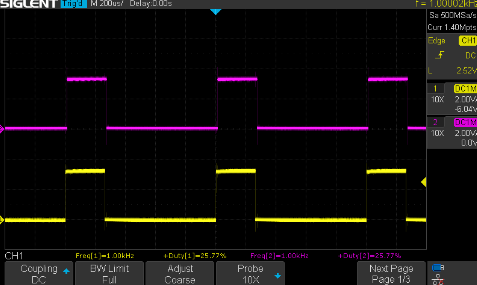
\includegraphics[keepaspectratio, height=2in]{figs/paper/bad_motors.png}
            \caption{Starting PWM of Arduino Motors}
            \label{fig:bad_motors}
        \end{figure}
        \begin{figure}[htbp]
            \centering
            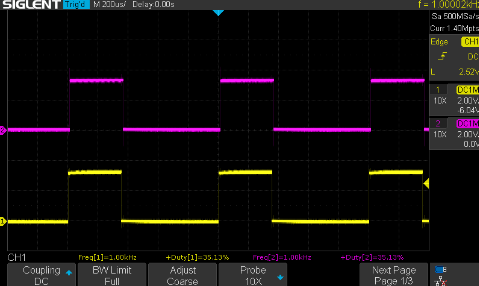
\includegraphics[keepaspectratio, height=2in]{figs/paper/good_motors.png}
            \caption{Starting PWM of Smart Motors}
            \label{fig:good_motors}
        \end{figure}

        \subsubsection{0.2.3.1.0 Hyperparameter Tuning}
        A way to improve the accuracy of the machine learning model was to appropriately tune the hyperparameters of EEGNet. This includes metrics such as the dropout rate, number of kernels, filtering methods used, and length of the kernel. A brute force method was tested wherein each combination of three possible values for 7 different hyperparameters was looped through and given an accuracy score from the model. Due to the time complexity of this test, only 3 members randomly chosen from the open source dataset were used. The results from this experiment are shown in Fig. \ref{fig:hyperparameter}. 
        \begin{figure}[htbp]
            \centering
            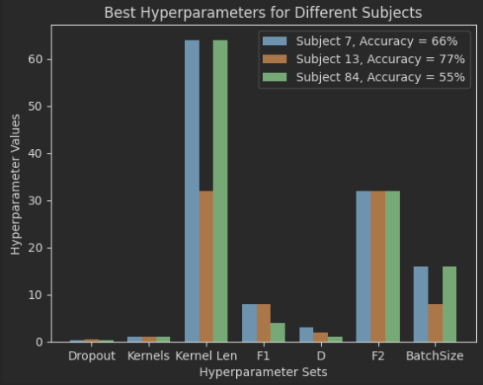
\includegraphics[keepaspectratio, height=2.7in]{figs/paper/hyperparameter_tuning.png}
            \caption{Best Hyperparameters for 3 different subjects}
            \label{fig:hyperparameter}
        \end{figure}
        
        The results from this experiment showed two main conclusions: every user for the system requires their own hyperparameter tuning and a need for a more efficient method of tuning hyperparameters. 

        \subsubsection{0.2.3.3 Electrode Placements}
        A large point of testing on this project was done to find the electrodes which elicited the most distinguishable response in the EEG waves. There are 64 possible areas to place electrode which monitor different parts of the scalp. To find the optimal placement of electrodes and then reconfigure our cap to match these placements would spell the best classification accuracy possible given our hardware. To test this, an open source dataset was used containing 109 different subjects performing MI EEG tasks while being monitored with a 64 channel EEG headset. Initial tests consisted of high level tools which analyzed the deep learning model and attempted to find the most important features from the trained model. These tools were not compatible with our model due to it being a novel, relatively recent machine learning model. The group opted to use a more simplistic model with built-in functionality for feature importance instead. A random forest classifier trained on the power spectral density estimation for each signal was used, due to the model requiring tabular data. This method was used for each subject in the dataset, and each electrode was given a score that corresponded to its importance in the analysis. The results from this configuration are shown in Fig. \ref{fig:bad_placements}. These results were not satisfactory, as electrode placements used in similar projects are shown in \ref{fig:good_placements}. The group opted to use the placements supported in the literature rather than from the results from the test.  
        \begin{figure}[htbp]
            \centering
            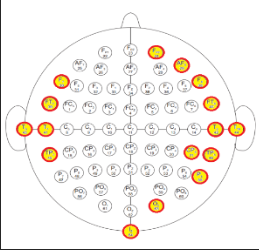
\includegraphics[keepaspectratio, height=3in]{figs/paper/bad_placements.png}
            \caption{Electrode Placements from RandomForestClassifier}
            \label{fig:bad_placements}
        \end{figure}
        \begin{figure}[htbp]
            \centering
            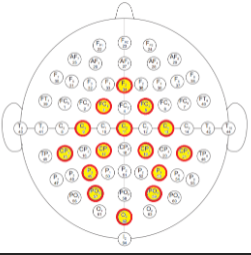
\includegraphics[keepaspectratio, height=3in]{figs/paper/good_placements.png}
            \caption{Electrode Placements from Literature}
            \label{fig:good_placements}
        \end{figure}

        \subsubsection{0.2.3.1.3 and 0.2.3.1.4 Filtering and Denoising}
        To improve the accuracy of the machine learning model, clean data is of the utmost importance. When working with non-invasive BCI techniques, the battle against noise is never ending. An EEG signal taken from the Ultracortex Mark IV which contains a noise spike is shown in Fig. \ref{fig:noisy_eeg}. 

        \begin{figure}[htbp]
            \centering
            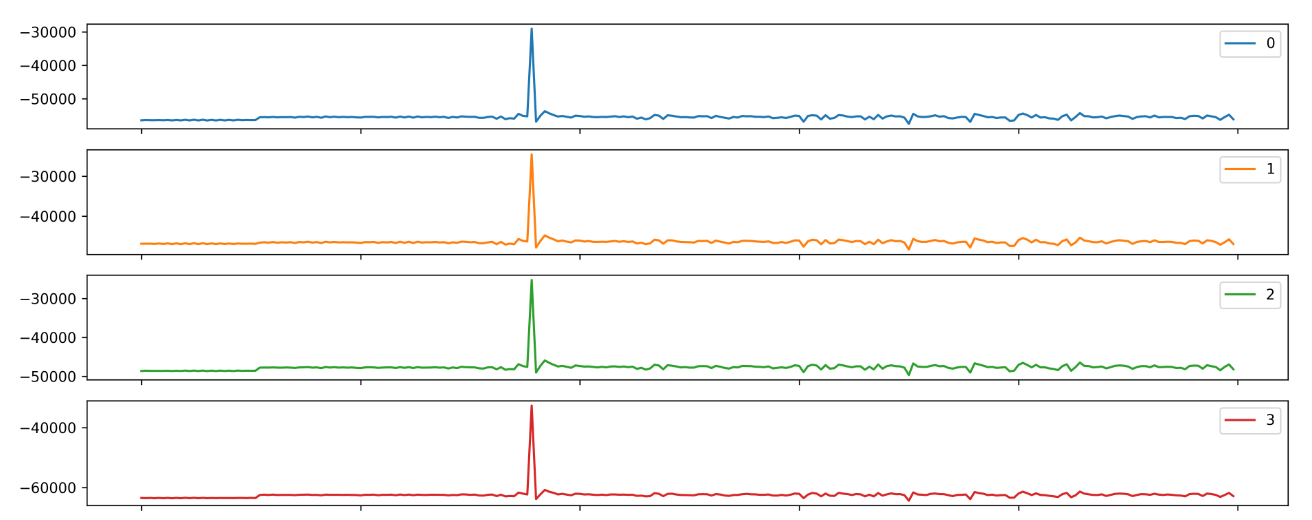
\includegraphics[keepaspectratio, height=3in, angle=90]{figs/paper/noisy_signal.png}
            \caption{Noise in EEG Signal}
            \label{fig:noisy_eeg}
        \end{figure}
        
        Tests were conducted in this project in which the data was fed through the model unfiltered, and then with filtered and denoising techniques. A self recorded dataset with the Ultracorted was used on data from a subject with minimal hair. The results were unexpected, no matter what filtering or denoising technique was used, the accuracy of the model did not significantly change. The results are shown in Fig. \ref{fig:filtering_denoising}. For the filtering, a bandpass filter from 8-59 Hz was used and for denoising, three techniques were employed:  a median filter, a rolling average filter, and a wavelet denoising filter.   
        \begin{figure}[htbp]
            \centering
            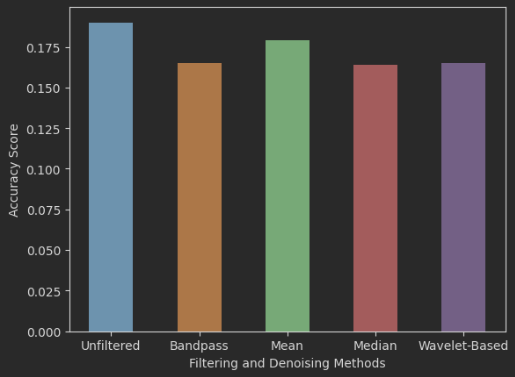
\includegraphics[keepaspectratio, height=2.3in]{figs/paper/filtering_methods.png}
            \caption{Accuracy Score from Different Filtering and Denoising Methods}
            \label{fig:filtering_denoising}
        \end{figure}

        An example of a electrodes 0 through three after they have passed through the bandpass filter is shown in Fig. \ref{fig:filtered_eeg} 

        \begin{figure}[htbp]
            \centering
            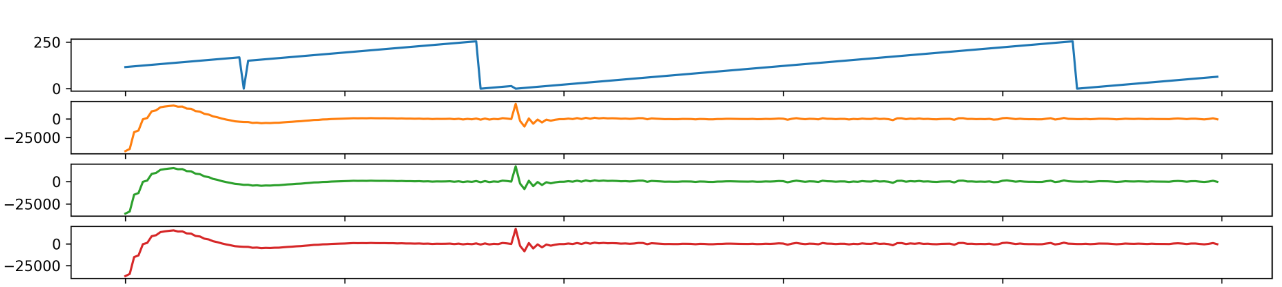
\includegraphics[keepaspectratio, height=1.7in, angle=90]{figs/paper/filtered_signal.png}
            \caption{Filtered EEG Signal}
            \label{fig:filtered_eeg}
        \end{figure}

        Upon further inspection with a confusion matrix, it was noticed that the model experienced a classification bias, shown in Fig. \ref{fig:confused_confusion}. The model’s accuracy score was low due to its lack of ability to distinguish between different signals. The model was trained to favor a particular output. This indicated to the group that more fine tuning to the model and better datasets were required.  
        \begin{figure}[htbp]
            \centering
            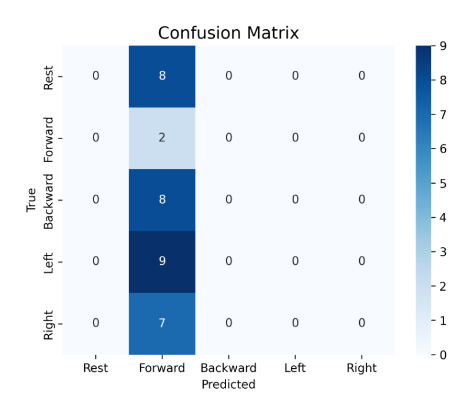
\includegraphics[keepaspectratio, height=2.7in]{figs/paper/bad_confusion.png}
            \caption{Classification Bias Confusion Matrix}
            \label{fig:confused_confusion}
        \end{figure}

    \subsection{Design Modifications and Final Product}
        Over the course of this project, we have laid the foundation for a non-invasive BCI Wheelchair. This includes a literature survey as well as the foundation for a fully realized system. The group has been limited by time and budget, allowing for some design modifications along the way.

        First and foremost is the computing system used. During the mid;point of the project, it was determined that the Orange Pi 5 was too cutting-edge due to a lack of support and documentation for the computer, notably communication with the Pi's GPIO pins. The decision was made to change the computing configuration to be distributed between a smaller embedded computer and a PC equipped with a GPU for faster procesing and development. A Raspberry Pi Pico paired with a Bluetooth module is employed, receiving commands from the PC application. To represent a motorized wheelchair in the prototype, the team decided to design a small 3D-printed RC car. Additionally, due to the longer-than-planned development of the machine learning model and the omission of the Orange Pi 5, the FPGA implementation was also excluded.

        The initial sensor design proposed four ultrasonic sensors and four infrared sensors positioned around the corners of the wheelchair prototype. Prior to this, a 2D LiDAR was favored for its 360-degree data field but was deemed too costly. Subsequently, a cost-effective 2D LiDAR was later discovered after the decision to use infrared sensors, prompting the team to revert to the 2D LiDAR. Unfortunately, during the latter stages of the project, developing a library compatible with the project was deemed unfeasible due to limitations of MicroPython used to program the Raspberry Pi Pico, coupled with time constraints. As a result, two ultrasonic sensors are currently being utilized to prevent head-on collisions. 

        Additionally, due to trouble with the sensor design, the decision was made to cut the backfeed of sensor data through the model. Not only would this have been very complex to implement, but with the design of the sensors changing, the design of the machine learning model would proportionally have to change. 
        
        DC motors remain a part of the project, now integrated with a gear reduction mechanism instead of a worm drive, specifically chosen to better suit the size of the RC wheelchair. This alteration was minor and was anticipated by the team when they selected DC motors with worm drive reduction gearing initially. 

            
    \subsection{Future Work}
        \subsubsection{Optimize Electrode Placements} 
        Work on this project has shown that electrode placements that elicit the most distinguished response to MI EEG signals differ from user to user. A method using a random forest was employed in this project, and gave unsatisfactory results. In a fully realized implementation, a better method to find the optimal electrode placements for a given user must be devised to garner a better classification accuracy. 
        \subsubsection{Explore Different Methods of classification}
        A compact CNN was employed for this project. While EEGNet worked well on a dataset which used a 64 channel EEG headset, it struggled with classification biases and low accuracy scores with a 16-channel headset. LSTMs and other machine learning classification methods should be explored for better classification accuracies. Complex forms of DSP should also be explored.
        \subsubsection{Improve Data Quality}
        To eliminate noise and generate distinguishable EEG signals, data quality should be of the utmost importance for future projects. More robust data free of noise is required for better results.
        \subsubsection{Explore Different Methods of Eliciting Signals}
        Motor imagery was the method of choice for distinguishing between different movements of the wheelchair. However, there exist other methods of “movement thoughts” that are possible, most notably P300.
        \subsubsection{Shared Control Strategies}
        For smooth, precise movements, better forms of shared control strategies should be employed in conjunction with the classified signals from the EEG cap. 3D LiDAR and other sensors should assist with movement. 
        \subsubsection{Embedded Implementation}
        For this project to be fully realized, a fully integrated, cohesive system must be employed on a motorized wheelchair. 
        
        
    

\section{Conclusion}
This project proposes a proof-of-concept non-invasive BCI wheelchair control. The resulting system utilizes an RC car able to be steered by both keyboard input and classified EEG signals. An altered electrode configuration of the Ultracortex Mark IV is used in conjunction with EEGNet to classify EEG signals from a user’s scalp. The system can be used by means of a graphical user interface application, taking the user through a training sequence followed by use of the system on a trained model. Non-invasive BCI technology suffers from many drawbacks, most notably noisy signals. The trained models struggled to perform well, suffering from classification biases. Further work on the project should include better shared control strategies, groups should optimize electrode placements and number of electrodes used, implement on an actual wheelchair, improve machine learning accuracy, and an embedded implementation. 
    
    

\section*{Acknowledgements}
\addcontentsline{toc}{section}{Acknowledgements}
The authors of this paper would like to thank Dr. Omar Eldash for his valuable help and insight on adequate hardware, Dr. Jose del Milan for his guidance in the field of EEG, Dr. Paul Darby for feedback and mentorship, and Dr. Magdy Bayoumi for his encouragement and sponsorship.  

\bibliographystyle{ieeetr}
\bibliography{refs}

\newpage
\begin{IEEEbiography}
    [{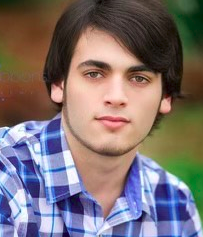
\includegraphics[width=1in,height=1.25in,clip,keepaspectratio]{figs/Gery.png}}]{Gerhort Alford}
    (S'19) Gerhort Michael Alford was born March 6, 1995. He was born and raised in Lockport, Louisiana, United States of America. Graduated from Central Lafourche Highschool in 2013 and is currently in his senior year in Electrical and Computer Engineering with minors in Mathematics, Renewable Energy, and Management at the University of Louisiana at Lafayette.
    % \vspace{-40mm}
\end{IEEEbiography}
\vspace{-100mm}
\begin{IEEEbiography}[{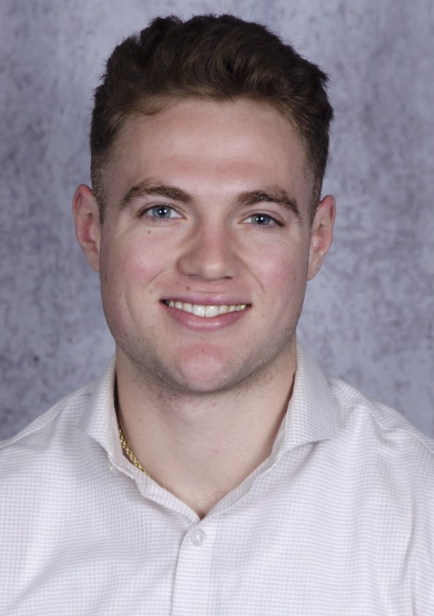
\includegraphics[width=1in,height=1.25in,clip,keepaspectratio]{figs/kaleb.png}}]{Kaleb Guillot}
(S'19) was born in Thibodaux, Louisiana in July of 2001. He was raised in a quiet subdivision, and attended high school at Thibodaux High, where he was a student athlete, playing both baseball and football. He excelled in his studies, and finished third in his class, graduating in the spring of 2019. He is currently a senior at the University of Louisiana at Lafayette, where he is employed as an Undergraduate Researcher on the PREFER project under Dr. Nian-Feng Tzeng. His current studies focus on data preprocessing and machine learning. 
\end{IEEEbiography}
\vspace{-100mm}
\begin{IEEEbiography}[{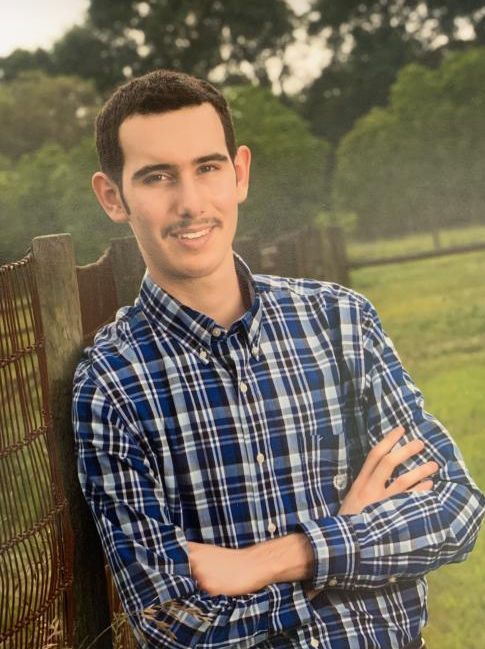
\includegraphics[width=1in,height=1.25in,clip,keepaspectratio]{figs/sam.png}}]{Samuel Whipp}
Samuel Whipp was born in Lafayette, Louisiana in April of 1997. He attended Westminster Christian Academy and played soccer there for three years, then graduated from CT Homeschool in 2015. He is currently a senior in Computer Science with an Information Technology concentration at University of Louisiana at Lafayette. He also is a self-employed business owner focusing on designing and fabricating 3D printed products.
    
\end{IEEEbiography}
\vspace{12pt}

\renewcommand{\appendixname}{Appendices}
\let\appendix\relax
\appendix

\clearpage
% \thispagestyle{empty}
% \mbox{}
\onecolumn
\begin{center}
    \addcontentsline{toc}{section}{Appendix A}
    \vspace*{4.5cm}
     {\Huge\bfseries Appendix A \par}
     \vspace{1cm}
    \textit{Scope of Work} \\
    \textit{Functional Requirements} \\
    \textit{Objective Tree} \\
    \textit{Level 0 and Level 1 Functional Block Diagrams}
\end{center}


\clearpage
\twocolumn

\renewcommand{\thesubsection}{A.\Alph{subsection}}
\title{Appendix A{\footnotesize \textsuperscript{*}}}
\section*{\textbf{Appendix A}}
    \setcounter{subsection}{0}
    \subsection{Scope of Work}
    The purpose of this project is to develop a proof-of-concept brain-controlled wheelchair. The specific individuals that would benefit from the technology used are those suffering from tetraplegia, a devastating neurodegenerative disorder that hinders a person's movement from the neck down. The main goal of this project is not to create a final market-ready product, but rather to establish the feasibility of the core functionalities of a brain-controlled wheelchair. 
    
    This project will include multiple testing phases, increasing in complexity with each phase. The initial tests will validate the decoded EEG signals using simple concepts, such as lighting LEDs. The next phase will include mapping the decoded signals an X-Y coordinate plane using a virtual dot moving on a display. This phase will be followed by testing the technology on a basic motorized device, such as a remote-controlled car. Once the movement of the car is refined and meets the team's satisfaction, the hardware will be incorporated into a wheelchair.

    The outline of the workflow of this project is outlined in \ref{fig:level-0} and \ref{fig:level-1}. An EEG cap will first receive the electric signals emanating from the user's scalp. These signals will be transmitted to an onboard minicomputer that will collaborate with external sensors and an FPGA to decode the signal into a command. A neural network on the minicomputer will orchestrate the decoding of the signal and transmitting the output command to the motor drivers, enabling wheelchair movement. 

    \subsection{Functional Requirements}
    \begin{enumerate}
        \item Read EEG signals
        \item Preprocess the signals
        \begin{enumerate}
            \item Remove noise
            \item Time window segmentation
        \end{enumerate}
        \item Feature Extraction
        \begin{enumerate}
            \item Power spectral density
            \item Entropy
            \item Coherence
        \end{enumerate}
        \item Command Generation
        \begin{enumerate}
            \item Map EEG signals into movement (left, right, forward)
        \end{enumerate}
        \item Wheelchair Control
        \begin{enumerate}
            \item Generated command will interface with the surrounding environment captured by sensors to interpret the intent of the user.
        \end{enumerate}
        \item Manual Overrides
        \begin{enumerate}
            \item Emergency override joystick
        \end{enumerate}
    \end{enumerate}

    
    \subsection{Objective Tree}
    Figure A.1 is an objective tree that provides visuals of what needs to be done in the project and the weight percentages of each task and sub-task. The task that will be the most labor intensive and has therefore been given the biggest percentage is the ability to accurately read and interpret the EEG signals. Without considerable effort given to this section, the project as a whole is not possible. The completion of this section is dependent on the quality of the literature review, which has also been given a considerable percentage. Since there is a limited number of projects similar to this, the broader categories of the research topics are listed. Once both of these objectives have been met, the final important objective to consider is the output, the movement of the wheelchair. The goal of this movement is to be indistinguishable from the movement of a normal motorized wheelchair at first glance. The motors need to function smoothly, safely, and effectively.
    
    
    
    \subsection{Block Diagrams}
        \subsubsection{Level 0}
        Figure A.2 is the level 0 block diagram, depicting the entire system as a single block with the required inputs and desired outputs. 
        \subsubsection{Level 1}
        Figure A.3 is the level 1 block diagram, going further into detail of  the inner workings of the motorized wheelchair. The most crucial aspect of this implementation is the minicomputer shown in the center. This device is responsible for orchestrating the system, taking in sensor data, EEG readings, commanding the FPGA and motor drivers, and displaying the user interface.  
    %%%%%%%%%%%%%%%%%%%%%%%%%%%%%%%%%%%%%%%%%%%%%%%%%%%%%%%%%%%%%%%%%%%%%%%%%%%%%%%%%%%%%%%%%%%%%%%
    \clearpage
    \onecolumn
    \setcounter{figure}{0}
    \renewcommand{\thefigure}{A.\arabic{figure}}
    \begin{figure}
        \centering
        % \centerline{\includegraphics[width=5in,height=6in,clip]{Objective_Tree_Figure_A.1.png}}
        \centerline{\includegraphics{figs/A/Objective_Tree_Figure_A.1.png}}
            \caption{Objective Tree}
            \label{fig:obj-tree}
            % cite with: s shown in Fig.~\ref{fig:level-0-block-diagram}, the 
    \end{figure}
    \begin{figure}
        \centering
        \centerline{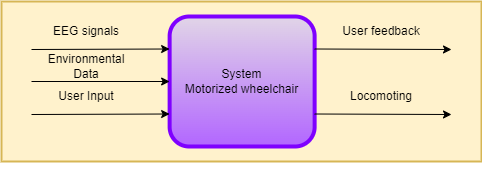
\includegraphics{figs/A/Level_0_Block_Diagram_Figure_A.2..png}}
        \caption{Level 0 Block Diagram}
        \label{fig:level-0}
    \end{figure}
    \begin{figure}[htbp]
            \centerline{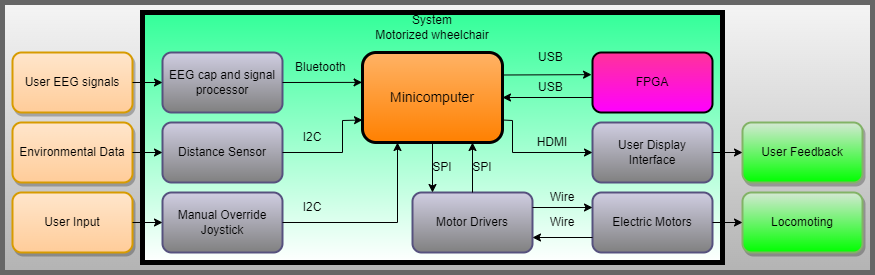
\includegraphics[height=2.4in,keepaspectratio]{figs/A/Level_1_Diagram_Figure_A.3_2.png}}
            \caption{Level 1 Block Diagram}
            \label{fig:level-1}
        \end{figure}    
    \twocolumn
    %%%%%%%%%%%%%%%%%%%%%%%%%%%%%%%%%%%%%%%%%%%%%%%%%%%%%%%%%%%%%%%%%%%%%%%%%%%%%%%%%%%%%%%%%%%%%%%

\clearpage
\onecolumn
\begin{center}
    \addcontentsline{toc}{section}{Appendix B}
    \vspace*{5cm}
     {\Huge\bfseries Appendix B \par}
     \vspace{1cm}
    \textit{Feasibility Analysis} \\
\end{center}
\clearpage
\twocolumn
\setcounter{section}{2}
\renewcommand{\thesubsection}{B.\Alph{subsection}}

\section*{\textbf{Appendix B}}

    % \renewcommand*{\subsection}
    \setcounter{subsection}{0}
    % \subsection{Feasibility Analysis}
        \subsection{Technological Feasibility}
        The technological feasibility of this project will heavily rely on the team's ability to develop a machine learning model that can interpret brain signals from the EEG cap and translate that into motion controls. The team has found several papers that have done such a thing \cite{robotic_architecture, learning_to_control, toward_brain_computer, self_paced, fpga_intel} so this aspect of the technical feasibility has been deemed feasible. The machine learning process will start in Python to test and train different models. This model will then be translated to C or C++ manually. If sufficient progress has been made, the model will be implemented onto an FPGA either manually or through use of a high level language synthesizer (HIS). This will translate the C or C++ code to an HDL language. While the team has not found anyone else doing this machine learning model implementation for a brain-controlled wheelchair specifically, documentation is available of models being translated to FPGA \cite{fpga_intel}.  

        Next in analyzing the technological feasibility is the motorized wheel chair. Motorized wheelchairs are commercially available for purchase; this aspect of the project is highly feasible. The team will build a motorized wheelchair purely for testing purposes to serve as a proof of concept or prototype.

        \subsection{Time Feasibility}
        The team has created a Gantt Chart, shown in Figure \ref{fig:gantt}, to determine the time feasibility of the project. The Gantt chart will keep us on task and ensure progress is kept on time. This chart shows goals for a time period and how long we have to complete them in an orderly manner. Through delegation of tasks, the team believes that this project is feasible with the time constraints. Kaleb Guillot is prioritizing his software contribution and Gerhort Alford is prioritizing his contributions to designing and implementing the hardware, with crossover in between where needed. The summer months may also be taken advantage of to continue to work on the project and problem-solve. 

        \subsection{Cost Feasibility}
        After arranging a rough bill of materials and taking into account some alternatives the team has concluded that the project will be well within the original budget of \$7,550.00. The rough bill of materials comes out to be {\$4,789.34}, which includes alternatives of the second most expensive parts which are the processors. Even though parts may change, the team is fairly certain that the initial budget will not be exceeded. The team has also been told by the project mentor and sponsor Dr. Magdy Bayoumi that the purchase of a data set for the machine learning model may also be required. He has specifically instructed us to contact him if this situation arises. With this, the cost feasibility of this project is feasible. The rough bill of materials can be seen in Fig. \ref{fig:bom}. 

        \setcounter{figure}{0}
        \renewcommand{\thefigure}{B.\arabic{figure}}
        \begin{figure}
        \centering
        \centerline{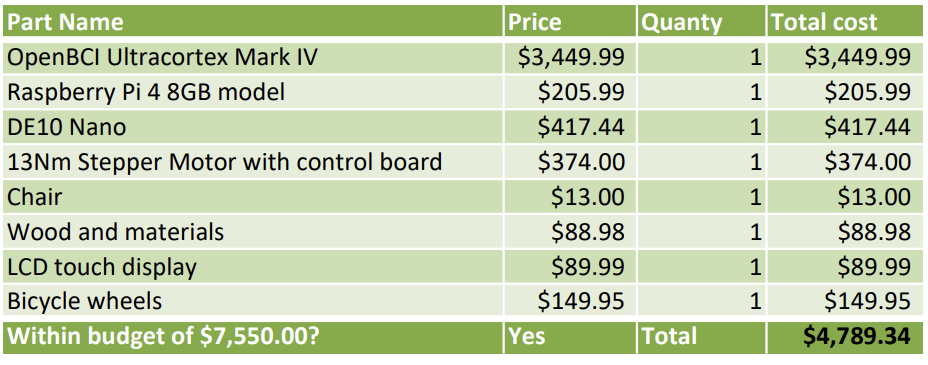
\includegraphics[height=1.35in, keepaspectratio]{figs/B/BOM.png}}
            \caption{Bill of Materials}
            \label{fig:bom}
            % cite with: s shown in Fig.~\ref{fig:level-0-block-diagram}, the 
        \end{figure}

        \subsection{Legal Consideration}
        Since this project is a prototype and not a final product marketed for public use, there is not worry about legal issues. If this was the final product, the team would have to follow the guide lines for the Food and Drug Administration (FDA) along with American with Disabilities act (ADA) in ensuring the wheelchair is safe and easy to use.

    \clearpage
    \onecolumn
    
    \begin{figure}
        \centering
        \centerline{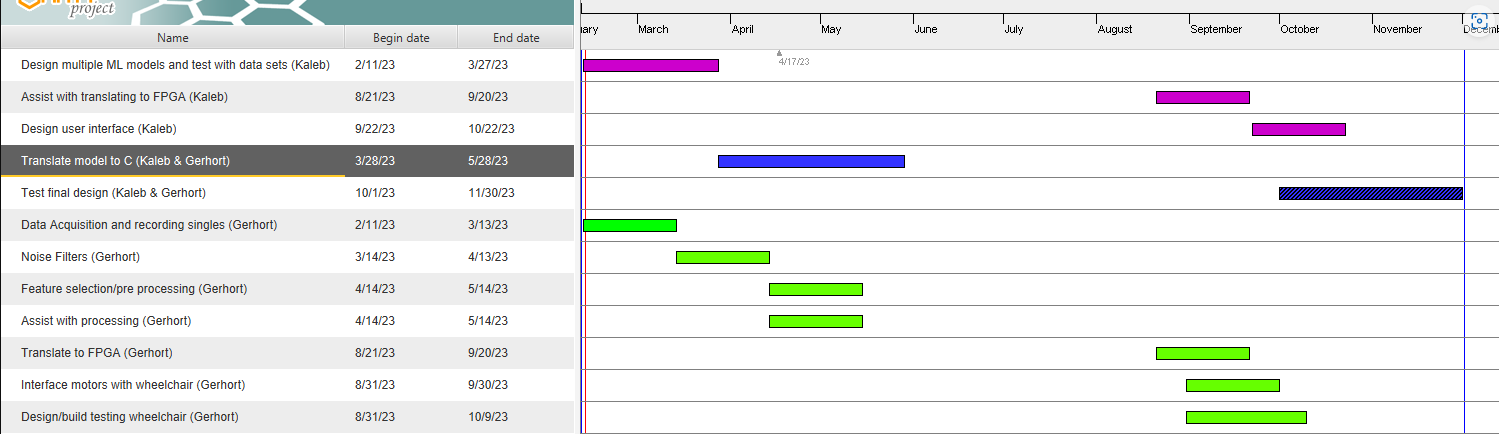
\includegraphics[angle=90, height=9in, keepaspectratio]{figs/B/gnatt.png}}
            \caption{Gantt Chart}
            \label{fig:gantt}
            % cite with: s shown in Fig.~\ref{fig:level-0-block-diagram}, the 
    \end{figure}
    \twocolumn
    
        
        
\clearpage
\onecolumn
\begin{center}
    \addcontentsline{toc}{section}{Appendix C}
    \vspace*{5cm}
     {\Huge\bfseries Appendix C \par}
     \vspace{1cm}
    \textit{Alternatives and Trade-offs} \\
\end{center}
\clearpage
\twocolumn

\clearpage
\setcounter{section}{3}
\renewcommand{\thesubsection}{C.\Alph{subsection}}
\section*{\textbf{Appendix C}}
        \setcounter{figure}{0}
        \renewcommand{\thefigure}{C.\arabic{figure}}
        \setcounter{table}{0}
        \renewcommand{\thetable}{C.\arabic{table}}
    \setcounter{subsection}{0}
    For both the software and hardware aspects of this project, there are many different, equally feasible paths that can be taken. The team has carefully considered each option and presents the current findings.
    
        \subsection{EEG Caps}
        Based on recommendations by peers and individual research, there are two companies for consideration that sell headsets which were previously used in related projects. These two companies are OpenBCI and G.Tec. OpenBCI is the more widely known of the two, selling caps which allow for full customization and having open-source software libraries beneficial for processing EEG signals. {OpenBCI's Ultracortex Mark IV is being considered by the group due to it having an adequate number of electrodes, an ability to be reassembled with 3-D printed parts, and an ability to work with any of OpenBCI's other microcontrollers.} G.Tec's headsets can be customized even further than what is possible with OpenBCI. G.Tec are the headsets of choice for experts in the field, such as that of \cite{learning_to_control}.  {Of G.Tec's selection, the team found the g.Nautilus Research headset to be suitable for this project due to its electrode placements and comparative affordability to G.Tec's other headsets.} However, due to the complexity and price tag of G.Tec headsets, the team has opted for an OpenBCI headset.
        
        As shown by Table \ref{tab:headsets}, there is one more company, EMOTIV, that sells a plug-and-play headset. Emotiv headsets are suitable for beginners in the field, such as students studying neuroscience. This headset is very high level and does not allow users to access the raw EEG data without a specialized license. The goal of this headset is to merely collect data, not manipulate it. Therefore, it is not suitable for this project in particular, nor does the team believe it suitable for any similar engineering and design work. This claim is backed by the work done in \cite{self_paced, biomedical-signal}. However, the software suite available for this headset is very eye-catching, allowing users to move virtual objects based on pre-designed models. The  {EMOTIV EPOC X} headset is available for the team's use, purchased by the mentor and sponsor. For these reasons, the team is developing an attraction using this headset for E\&T Week. 
        
        \subsection{Minicomputers}
        The processing is a critically important part of this project as it employs a pre-trained machine learning model, interpreting the brain signals from the EEG cap. This requires several powerful, portable processing units and pieces of hardware. Table \ref{tab:minicomputer} presents the current findings. The team is considering several minicomputers, weighing the power of their CPU, availability of peripherals, available documentation, and accessibility. The three currently in consideration are the Jetson nano, Orange Pi 5, and Raspberry Pi 4. The team's processing needs are similar to that of image processing; the incoming signals from the EEG cap will be treated like an image and will be compared to the movement signals. This process needs to be as fast as possible, so when the user of the wheelchair wants to move forward they can move nearly instantaneously. These minicomputers, however, are not powerful enough to process a robust model in an efficient manner. The processors will need to be supplemented with another piece of hardware, such as an FPGA, that will handle the simple, repetitive calculations. 
        
        With these factors in mind, the team has carefully weighed the options based on recommendations by peers and independent research. The first option was the popular Raspberry Pi 4, with the pull of a wealth of documentation. This processor, however, is currently hard to obtain due to shortages, leading us to the Orange Pi 5. The Orange Pi 5 is akin to the Raspberry, but with the addition of built in tensor processing capabilities with an ARM Mali-G610 MP4 GPU. The final option is the Jetson Nano. The Nano is powerful enough to run Ubuntu, and only comes in at a slightly higher price than the Orange Pi 5. However, due to the ease of use and increased RAM of the Orange Pi 5, it is a front runner.
        
        \subsection{Motors}
        On the wheelchair, two motors will be employed to drive two of the wheels of the wheelchair. The motors will be responsible for receiving the signal from the processing unit and outputting accurate and reliable movement. This requires motors that are capable of producing high torque at slow speeds. The position of the motor needs to be known, keeping tabs on the traction of the wheels and having the ability to know the actual speed compared to the outputted, desired speed. This can allow for adjustments and calibrations to be made automatically. 
        
         {There are three types of motors under consideration. They are servo, stepper, and DC motor with a worm drive.} These motors are displayed in Table \ref{tab:motors}.  {The team has decided to use a DC motor with a worm drive. This type of motor consists of a brushed DC motor that drives a reduction worm gear. In a worm gear system, a screw-like gear drives a helical gear at a much slower speed, but with significantly higher torque than the motor shaft. The team has chosen this option for three main reasons. Firstly, the worm drive significantly reduces the motor's revolutions per minute while increasing its torque output, which is ideal for the slow speed requirements of a wheelchair. Secondly, the worm gear system makes it difficult to turn the output shaft, which is beneficial for ensuring that the wheelchair remains stationary if the power supply fails. Finally, the cost of this option is the most affordable, even with the added expense of the necessary hardware for feedback.} 

        \subsection{FPGAs}
        There are two main FPGA manufacturers: Xilinx which is owned by AMD and Altera which is owned by Intel. The analysis of the alternatives and tradeoffs for these two manufacturers are shown in Table \ref{tab:fpga}. There are many different boards these manufacturers make, each with similar capabilities for the purposes of this project. While Intel has a larger selection, Xilinx is the current favorite due to the ability to coincide with the other components of the design. The main concern for the project is the integrated synthesis environment (ISE) both these manufacturers use. Both can be downloaded and used for free, so price is not a concern. These ISEs will be able to translate the machine learning model in C++ to VHDL, Verilog, or System Verilog. Since the team has access to boards from both manufacturers, it will be easy to test which ISE is better at converting the machine learning model to a hardware description language like Verilog, System Verilog, or VHDL. From each of these manufacturers, the two boards the team has held in consideration are the Xilinx TUL PYNQ-Z2 and the Altera DE10-Nano. Both have similar hardware available, however the  {group has elected to use the Xilinx TUL PYNQ-Z2}  due to its ease of use and the ability to interface with external minicomputers. 

        \subsection{Environmental Sensors}
            \subsubsection{Distance Sensors}
            For the wheelchair to gather information about the surrounding environment, sensors that measure distance must be used to detect any potential obstacles. The sensors that were considered by the team are shown in Table \ref{tab:sensors}. They include ultrasonic, infrared, LIDAR, and cameras. 
            
            Ultrasonic sensors emit high-frequency sound waves that detect the reflected sound to calculate distance. These sensors are cheap and have a wide field of view, however they are susceptible to interference, have limited resolution, and have limited accuracy. 
    
            Infrared sensors detect the presence of obstacles through emitting infrared radiation and then calculating the reflected radiation. They are cheap, have good range, and are suitable for indoor use, which is beneficial for a wheelchair that will likely spend a considerable amount of time indoors. However, infrared sensors have a limited field of view, are affected by temperature, and have limited accuracy.
    
            LIDAR sensors use light to detect the distance and location of objects in the environment. These sensors are often used on similar projects \cite{learning_to_control, openbci-research, collab_controller} as they are accurate, have a long range, are capable of 3-D mapping, and are resistant to environmental interference. It comes as no surprise that the disadvantages of these sensors are their cost and required processing power.
    
            Cameras are another popular choice for similar projects \cite{learning_to_control, openbci-research}. Cameras are a similar story to LIDAR, as they have many of the same capabilities with the additional ability to distinguish color and process images. The disadvantages are similar as well, as cameras require high processing power, high cost, and high overhead. 
    
            After careful consideration, the team has elected to use a combination of ultrasonic and infrared sensors. These sensors have low form factors, are lightweight, and are low-cost. They function well at similar ranges, with ultrasonic sensors working well with hard surfaces and infrared sensors working well with reflective surfaces. They will work to compensate for the limitations of each other, as each sensor's functionality declines in different environments. 

            \subsubsection{ {Inertial Measurement Units}}
            Information about the wheelchair's orientation and acceleration can prove to be key safety features when interfaced with the motor drivers and braking system. These sensors will also provide another layer of feedback to the ensure that the outputted commands sent to the motor drivers are adequately performed by the motors. The analysis of different types of inertial measurement units (IMUs) are shown in Table \ref{tab:imu}, referencing three types of units. They are the micro-electro-mechanical system (MEMS) IMU, fiber optic gyro (FOG) IMU, and the ring laser gyro (RLG) IMU. This subsection will explore the key differences between these three IMUs.

            The MEMS IMU is best known for its applications in mobile devices, such as smart phones and smart watches. To take measurements of acceleration and rotation, they utilize tiny mechanical structures that make the MEMS lightweight and affordable. The accuracy of these IMUs is normally inferior to other types of IMUs, as they are susceptible to noise and other sources of error. While these IMUs require precise calibration and filtering, they are typically easily integrated with other sensors and electronics, making them suitable for this project.

            The FOG IMU uses fiber optics to detect changes in the orientation of a system. They consist of a coil of optical fiber that is wound around a rotating spindle. The measurements are recorded through the roation of the spindle which causes the light passing through the fiber to experience a phase shift. FOG IMUs are often used in applications where accuracy and precision are quintessential, such as in aerospace and robotics. They are very reliable, offering continuous measurement of rotation rates and high accuracy, even in harsh conditions. These IMUs are more expensive, have a larger form factor, and require additional measures to maintain stability over time. Due to high priority of safety of this project, these sensors would be beneficial to include.

            The RLG IMU use ring laser gyros to measure rotation. They consist of a closed loop of laser light that is split into two beams traveling in opposite directions. When the loop rotates, it causes a phase shift in the two beams, capturing the rotation. They are akin to the FOG IMU in their reliability, accuracy, need for additional measures to maintain stability, and high price. They excel compared to FOG IMUs in their compact and lightweight design, and far exceed MEMS IMUs in their continuous measurements and stability over time. For a commercial application of this project, these sensors would be beneficial to include.  

            After consideration, the group has opted for the MEMs IMU due to its adequate accuracy and reliability, and it being more affordable and easy to work with compared to the RLG and FOG IMUs.

        \subsection{ {Software}}
            \subsubsection{Machine Learning}
            In order to correctly classify the user's intent while wearing the EEG cap, a machine learning model must be trained. This model needs to classify input from the EEG cap and environmental sensors quickly and effectively, while remaining simplistic enough to fit on the onboard minicomputer. There are four models that the team is considering: Random Forest, Convolutional Neural Network (CNN), Long Short-Term Memory (LSTM), and Gated Recurrent Unit (GRU). 
            
            A Random Forest is a type of ensemble learning algorithm that combines multiple decision trees to make predictions. This means that multiple algorithms will be combined in order to make a final prediction. This is the most robust of the options, as a Random Forest can encapsulate one or more of the other models under consideration. A CNN is a very popular model often used for classifying images by performing convolutional calculations on subsets of the pixels in the image. This model is the most simple of the ones under consideration and has the downside of not capturing the temporal locality of predictions. An LSTM is a type of Recurrent Neural Network (RNN) that captures temporal locality through its ability to handle long-term dependencies in sequential data. A single LSTM block contains three main components: an input gate, output gate, and a forget gate. This model is very popular and robust, making accurate predictions but requiring powerful hardware to run efficiently. A GRU is similar to an LSTM in capturing temporal locality, however it is computationally more simple. These networks only have two gates: an update gate and a reset gate. 
            
            These options are displayed in Table \ref{tab:ml-tbl}, showing a brief description, the pros and cons, and a rationale of the team's choice. The team has opted to use a CNN to classify the EEG and sensor data, as the team is familiar with this model and believes it be sufficient for use in this project.
        \onecolumn
        \renewcommand{\arraystretch}{3}
        \setlength{\arrayrulewidth}{1.5pt}

        \begin{table}[htbp]
            \centering
            \begin{tabular}{|>{\raggedright\arraybackslash}c|>{\raggedright\arraybackslash}p{0.25\linewidth}|>{\columncolor{orange!20}\raggedright\arraybackslash}p{0.25\linewidth}|>{\raggedright\arraybackslash}p{0.25\linewidth}|}
                \hline
                \textbf{\textit{EEG Caps}} & \textbf{EMOTIV EPOC X} & \textbf{Ultracortex Mark IV} & \textbf{g.NAUTILUS} \\
                \hline

                \rule{0pt}{4cm}\multirow{-3}{*}{\textit{Picture}} & \adjustbox{center}{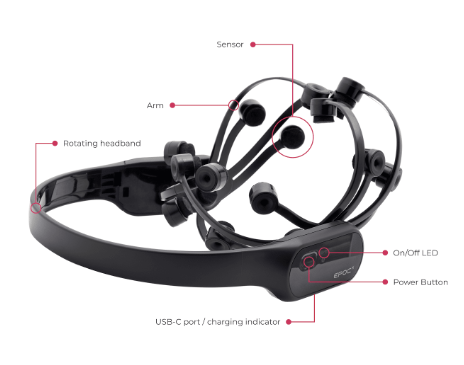
\includegraphics[height=1.3in,keepaspectratio]{figs/C/alts-pics/emotiv.png}} & \centering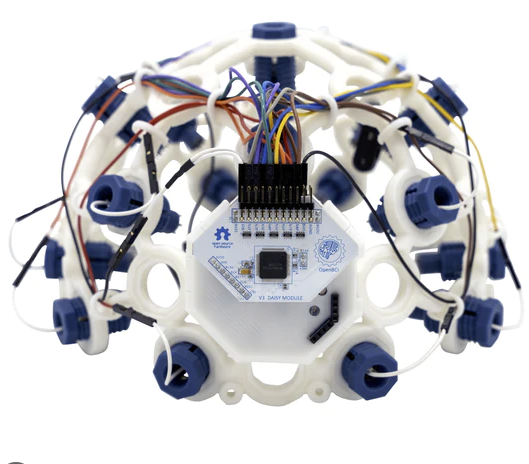
\includegraphics[height=1.3in, keepaspectratio]{figs/C/alts-pics/ultracortex.png} & \adjustbox{center}{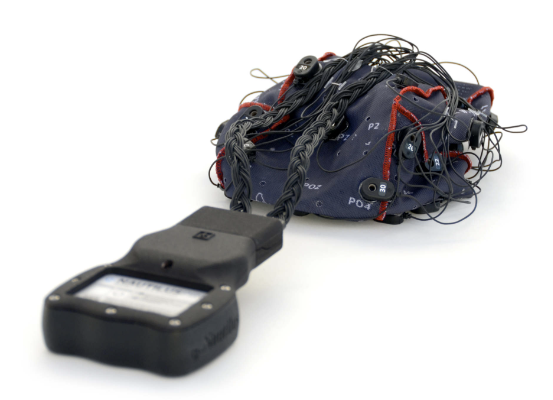
\includegraphics[height=1.3in, keepaspectratio]{figs/C/alts-pics/g-tec.png}}
                
                \\
                
                \textit{Description and Specs} & Lightweight EEG cap with 14 channels & Highly customizable 16 channel EEG cap & Professional grade 4-64 channel EEG cap \\ 

                \hline

                \multirow{3}{*}{\textit{Pros}} & \begin{itemize}
                                    \item Beginner friendly software
                                    \item Has 5 trainable models to use, no machine learning required
                                    \item Available APIs for customized applications
                                \end{itemize}
                            &  \begin{itemize}
                                \item Very customizable and easy to make modifications
                                    \item Good documentation and software libraries available in many programming languages
                                \end{itemize}
                            & \begin{itemize}
                                \item Professional build quality
                                \item Highly customizable
                                \item Available Software libraries and APIs
                            \end{itemize}
                            \\

                \multirow{3}{*}{\textit{Cons}} & \begin{itemize}
                                    \item Fragile
                                    \item Access to raw EEG data is locked behind paywall
                                    \item Must be connected to wifi at all times
                                    \item Electrodes must be constantly adjusted
                                \end{itemize}

                            & \begin{itemize}
                                    \item Some self-assembly required
                                    \item Cheap, 3D printed build quality
                                \end{itemize}

                            & \begin{itemize}
                                    \item Very expensive
                                    \item Requires extensive knowledge of the field for proper use
                                \end{itemize}
                                \\
                \multirow{2}{*}{\textit{Rationale}} & EMOTIV headsets are not intended to be used for technological research 
                & OpenBCI has a wealth of software and hardware tools available and its intended use is for technological research
                & Out of price range \\
                \hline
            \end{tabular}
            % \captionsetup{skip=10pt}
            \caption{EEG Headset Alternatives and Tradeoffs}
            \label{tab:headsets}
        \end{table}

        \begin{table}[htbp]
            \centering
            \begin{tabular}{|>{\raggedright\arraybackslash}c|>{\raggedright\arraybackslash}p{0.25\linewidth}|>{\columncolor{orange!20}\raggedright\arraybackslash}p{0.25\linewidth}|>{\raggedright\arraybackslash}p{0.25\linewidth}|}
            \hline
            \textbf{\textit{Minicomputers}} & \textbf{Raspberry Pi 4} & \textbf{Orange Pi 5} & \textbf{Jetson Nano} \\
            \hline
            \rule{0pt}{4cm}\multirow{-3}{*}{\textit{Picture}} 
                & \centering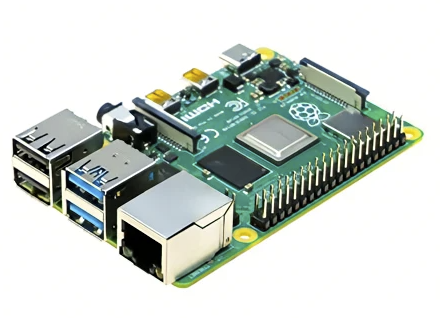
\includegraphics[height=1.3in,keepaspectratio]{figs/C/alts-pics/raspberry.png}& \centering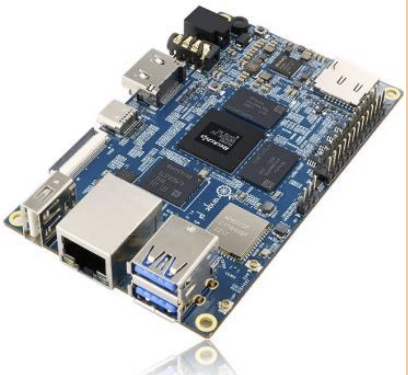
\includegraphics[height=1.3in,keepaspectratio]{figs/C/alts-pics/orange.png} & \adjustbox{center}{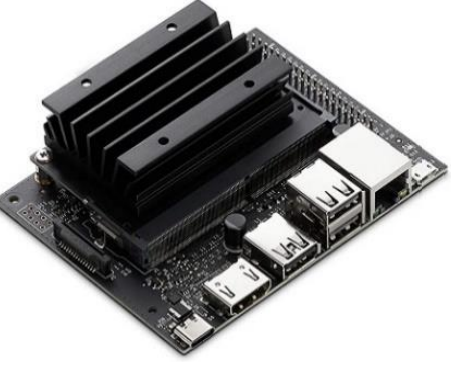
\includegraphics[height=1.3in,keepaspectratio]{figs/C/alts-pics/jetson.png}} \\

            \multirow{6}{*}{\textit{Description and Specs}} & Minicomputer that runs a Debian Linux based operating system \begin{itemize}
                                \item CPU: Quad core Cortex-A72 (ARM v8) 64-bit SoC @ 1.8GHz
                                \item RAM: 1-8 GB SDRAM
                                \item 1 x USB C port
                                \item 2 x micro HDMI ports
                                \item 2 x USB 3.0 ports
                                \item 2 x USB 2.0 ports
                                \item 2-lane MIPI DSI display port
                                \item Gigaabit Ethernet port
                                \item 2.4GHz and 5.0 GHz IEEE 
                                \item 802.11ac wireless
                                \item Bluetooth 5.0
                                \item 26 GPIO headers
                            \end{itemize}
                        & Minicomputer that runs Android based operating system
                        \begin{itemize}
                            \item CPU: Rockchip RK3588S octa-core 64-bit processor, Main frequency up to 2.4GHz
                            \item RAM size: 4-32GB LPDDR4
                            \item GPU: Arm Mali-G610 MP4
                            \item NPU: Built-in AI accelerator NPU with up to 6 TOPS, supports INT4/INT8/INT16 mixed operation
                            \item PMU: RK806-1
                            \item Micro-SD card slot
                            \item 1 x HDMI 2.1 port
                            \item 2 x USB 3.0 port
                            \item 1 x USB 2.0 port
                            \item 1 x Ethernet port
                            \item M.2 M-KEY Socket
                            \item 26 GPIO headers
                        \end{itemize}
                        
                        & Minicomputer that runs OS based on Ubuntu 10.04 (Linux4Tegra)
                        \begin{itemize}
                            \item CPU: Quad-core ARM Cortex-A57 
                            \item MPCore processor
                            \item RAM size: 4 GB 64-bit LPDDR4
                            \item 16GB eMMC5.1
                            \item 2 x USB 3.0
                            \item 1 x USB 2.0
                            \item 1 x HDMI 2.0
                            \item 1 x USB Micro-B
                            \item 26 GPIO pins
                            \item M.2 Key E slot
                        \end{itemize}
                        
                        \\ 
            \hline
            \textit{Cost} & \$75.00-\$205.00 & \$130.00 & \$149.00 \\

            \multirow{3}{*}{\textit{Pros}} & \begin{itemize}
                                \item Good documentation
                                \item Built in WiFi and Bluetooth
                                \item 4 USB Ports
                            \end{itemize}
                        & \begin{itemize}
                            \item Good availability
                            \item Hardware capable of machine learning
                            \item Most powerful CPU
                        \end{itemize}
                        
                        & \begin{itemize}
                            \item Good availability
                            \item Hardware capable of machine learning
                            \item Most powerful GPU
                        \end{itemize}
                        \\
            \multirow{3}{*}{\textit{Cons}} 
                & 
                \begin{itemize}
                    \item Shortages; hard to obtain
                    \item Need external hardware to perform machine learning
                \end{itemize}
                & 
                \begin{itemize}
                    \item New product, not well documented
                    \item No built in WiFi or Bluetooth
                \end{itemize}
                & 
                \begin{itemize}
                    \item Not well documented
                \end{itemize}
                \\
            \multirow{2}{*}{\textit{Rationale}} 
                & Not capable of running machine learning algorithm on its own
                & Hardware is capable of performing machine learning. Available to the group. 
                & Not available to the group \\
            \hline
            \end{tabular}
            \caption{Minicomputer Alternatives and Tradeoffs}
            \label{tab:minicomputer}
            
        \end{table}

        \begin{table}[htbp]
            \centering
            \begin{tabular}{|>{\raggedright\arraybackslash}c|>{\raggedright\arraybackslash}p{0.25\linewidth}|>{\raggedright\arraybackslash}p{0.25\linewidth}|>{\columncolor{orange!20}\raggedright\arraybackslash}p{0.25\linewidth}|}
            \hline
                 \textbf{\textit{Motor Type}} & \textbf{Servo} & \textbf{Stepper} & \textbf{DC Motor with Worm Drive}  \\
            \hline
                 \rule{0pt}{4cm}\multirow{-4}{*}{\textit{Picture}} & \centering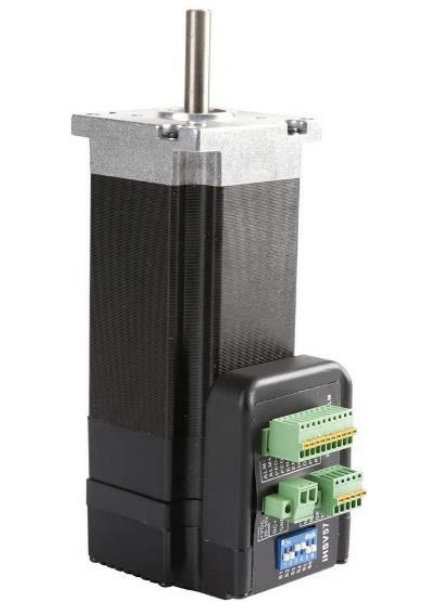
\includegraphics[height=1.5in, keepaspectratio]{figs/C/alts-pics/servo.png} & \adjustbox{center}{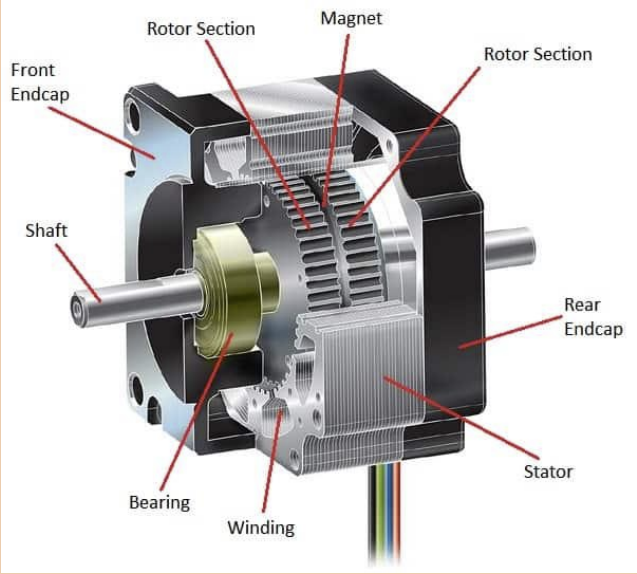
\includegraphics[height=1.5in, keepaspectratio]{figs/C/alts-pics/stepper.png}} & \adjustbox{center}{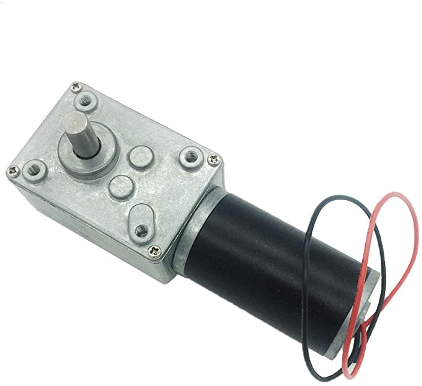
\includegraphics[height=1.5in, keepaspectratio]{figs/C/alts-pics/worm_drive.png}}\\

                \multirow{1}{*}{\textit{Description and Specs}} 
                & Use radially magnetized rotors to turn 
                & Motor rotation is controlled by an electric pulse
                & Brushed DC motor with a worm drive reduction gear \\
            \hline
                \textit{Cost Range} & \$100.00 - \$400.00 & \$85.00 - \$200.00 & \$12.00 - \$60.00 \\
                \multirow{2}{*}{\textit{Pros}} 
                & 
                \begin{itemize}
                    \item Closed loop feedback
                    \item High torque at high speeds
                \end{itemize}
                & 
                \begin{itemize}
                    \item High torque at low speeds
                    \item Lower cost
                    \item Quick response
                    \item Smaller form factor
                \end{itemize}
                &
                \begin{itemize}
                    \item High torque at low speeds
                    \item Lowest cost
                    \item Will not turn without power. Wheelchair will stay in place if power is lost
                \end{itemize}
                \\
            \multirow{3}{*}{\textit{Cons}} 
                &
                \begin{itemize}
                    \item Slow response
                    \item Longer body
                    \item Higher Cost
                    \item Low torque at low speeds
                \end{itemize}
                &
                \begin{itemize}
                    \item No feedback; needed for this project's design needs
                    \item Lower torque at high speeds
                \end{itemize}            &
                \begin{itemize}
                    \item Need to add feedback for wheelchair, requires extra components
                    \item Many of these motors are only capable of low speeds due to gear reduction. 
                \end{itemize}
                \\
            \multirow{1}{*}{\textit{Rationale}} 
                & External braking mechanism would be needed. Does not automatically brake without
                & Spins freely without power 
                & Automatically brakes when no power is supplied. Low speed with high torque.  \\
            \hline
                 
            \end{tabular}
            \caption{Motor Alternatives and Tradeoffs}
            \label{tab:motors}
        \end{table}

        \begin{table}[htbp]
            \centering
            \begin{tabular}{|c|>{\columncolor{orange!20}\raggedright\arraybackslash}p{0.4\linewidth}|>{\raggedright\arraybackslash}p{0.4\linewidth}|}
            \hline
                 \textbf{\textit{FPGAs}} & \textbf{TUL PYNQ-Z2} & \textbf{DE10-Nano}  \\
            \hline
                 \rule{0pt}{4.5cm}\multirow{-4}{*}{\textit{Picture}} & \adjustbox{center}{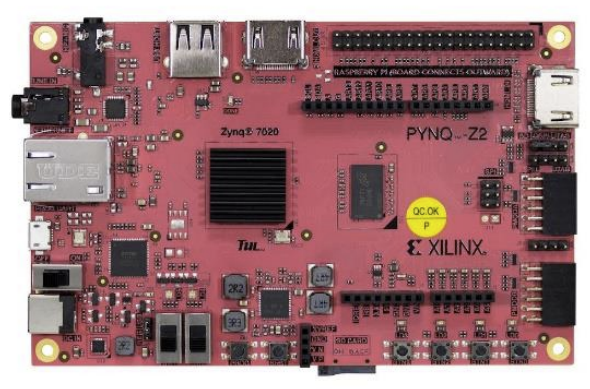
\includegraphics[height=1.5in, keepaspectratio]{figs/C/alts-pics/tulpynq.png}} & \adjustbox{center}{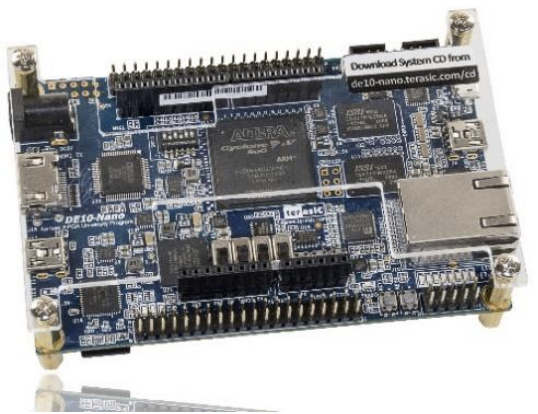
\includegraphics[height=1.5in, keepaspectratio]{figs/C/alts-pics/de10.png}}
                 \\

                \multirow{3}{*}{\textit{Description and Specs}} 
                &
                Xilinx FPGA with a dual core ARM cortex A9 processor. 
                \begin{itemize}
                    \item 85K logic cells (13300 logic slices, each with four 6-input LUTs and 8 flip-flops)
                    \item 220 DSP slices
                    \item 630 KB of fast block RAM
                \end{itemize}
                &
                Altera FPGA with a dual core ARM cortex A9 processor.
                \begin{itemize}
                    \item Logic elements (LE): 110 K LE
                    \item 5,570 kilobits memory
                    \item 224 18 x 19 multipliers
                    \item 112 variable precision DSP blocks
                    \item 6 phased-locked loops (PLL)
                    \item 145 user-defined I/O
                \end{itemize}
                \\
            \hline
                \textit{Cost Range} & \$123.00 & \$417.44 \\
                \multirow{3}{*}{\textit{Pros}} 
                &
                \begin{itemize}
                    \item Can run programs written in Python
                    \item Lower Price
                    \item Has Raspberry Pi style 26 pin GPIO headers
                    \item Developer tools can be used for free
                \end{itemize}
                & 
                \begin{itemize}
                    \item In stock
                    \item Large user community with copious amount of documentation
                    \item Many connections for peripherals
                \end{itemize}\\
                \multirow{2}{*}{\textit{Cons}} 
                &
                \begin{itemize}
                    \item Not as much documentation
                    \item Hard to find
                \end{itemize}
                &
                \begin{itemize}
                    \item Expensive
                    \item Does not support Python
                    \item Developer tools are limited
                \end{itemize}
                \\
            \multirow{1}{*}{\textit{Rationale}}
                & Compatible with the chosen minicomputer and much simpler to work with.
                & Lower level and much more difficult to work with. \\ 
            \hline
                 
            \end{tabular}
            \caption{FPGA Alternatives and Tradeoffs}
            \label{tab:fpga}
        \end{table}
        
        \begin{table}[htbp]
            \centering
            \begin{tabular}{|c|>{\columncolor{orange!20}\raggedright\arraybackslash}p{0.18\linewidth}|>{\columncolor{orange!20}\raggedright\arraybackslash}p{0.18\linewidth}|>{\raggedright\arraybackslash}p{0.18\linewidth}|>{\raggedright\arraybackslash}p{0.18\linewidth}|}
            \hline
                 \textbf{\textit{Sensor}} & \textbf{Ultrasonic} & \textbf{Infrared} & \textbf{LIDAR} & \textbf{Camera}  \\
            \hline
                 \rule{0pt}{3cm}\multirow{-3}{*}{\textit{Picture}} & \adjustbox{center}{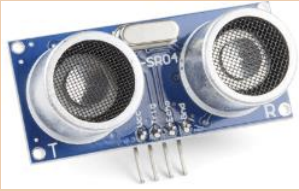
\includegraphics[height=1in, width=1.3in]{figs/C/alts-pics/ultrasonic.png}}& \adjustbox{center}{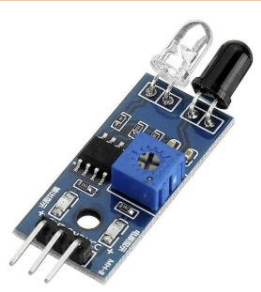
\includegraphics[height=1in]{figs/C/alts-pics/infrared.png}} & \adjustbox{center}{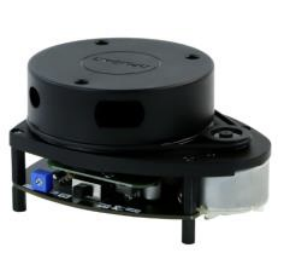
\includegraphics[height=1in]{figs/C/alts-pics/lidar.png}} & \adjustbox{center}{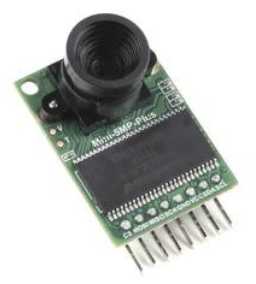
\includegraphics[height=1in]{figs/C/alts-pics/camera.png}}\\

                \multirow{2}{*}{\textit{Description and Specs}} & Emits high frequency sound waves that detect the reflected sound & Emits infrared radiation and then detects the reflected signal & Emits laser light and detects the reflected signal & Captures and records light that enters the lens \\
            \hline
                \textit{Cost Range} & \$3.75 - \$34.95 & \$3.95 - \$26.75 & \$25.99 - \$999.00 & \$59.99 - \$800.00 \\
                \multirow{2}{*}{\textit{Pros}} 
                &
                \begin{itemize}
                    \item Affordable
                    \item Wide field of view
                \end{itemize}
                & 
                \begin{itemize}
                    \item Affordable
                    \item Suitable for indoor use
                \end{itemize}
                &
                \begin{itemize}
                    \item Accurate
                    \item Long range
                    \item 3D mapping
                    \item Resilient
                \end{itemize}
                & 
                \begin{itemize}
                    \item Accurate
                    \item Object Detection
                \end{itemize}
                \\
                \multirow{2}{*}{\textit{Cons}} 
                & 
                \begin{itemize}
                    \item Susceptible to interface
                    \item Limited resolution
                    \item Limited accuracy
                \end{itemize}
                & 
                \begin{itemize}
                    \item Limited field of view
                    \item Affected by temperature
                    \item Limited accuracy
                \end{itemize}
                & 
                \begin{itemize}
                    \item High cost
                    \item High processing power
                    \item High overhead
                \end{itemize}
                & 
                \begin{itemize}
                    \item High cost
                    \item High processing power
                    \item High overhead
                \end{itemize}
                \\
            \multirow{1}{*}{\textit{Rationale}}
                & Simple, effective, easy to work with
                & Simple, effective, easy to work with
                & Complex, requires a lot of software overhead, and  expensive.
                & Complex and requires a lot of software overhead
                \\
            \hline
                 
            \end{tabular}
            \caption{Environmental Sensor Alternatives and Tradeoffs}
            \label{tab:sensors}
        \end{table}
        
        \begin{table}[htbp]
            \centering
            \begin{tabular}{|>{\raggedright\arraybackslash}c|>{\columncolor{orange!20}\raggedright\arraybackslash}p{0.25\linewidth}|>{\raggedright\arraybackslash}p{0.25\linewidth}|>{\raggedright\arraybackslash}p{0.25\linewidth}|}
            \hline
            \textbf{\textit{IMUs}} & \textbf{MEMs} & \textbf{FOG} & \textbf{RLG} \\
            \hline
            \rule{0pt}{4cm}\multirow{-3}{*}{\textit{Picture}} & \centering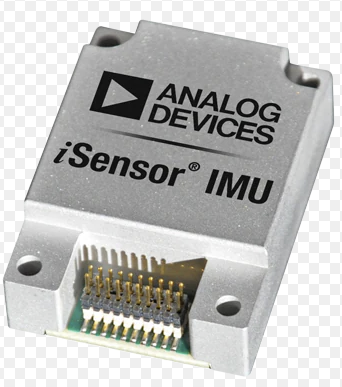
\includegraphics[height=1.3in,keepaspectratio]{figs/C/alts-pics/mems.png}& \centering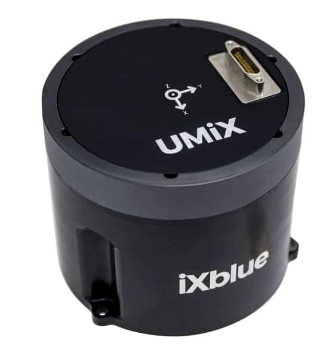
\includegraphics[height=1.3in,keepaspectratio]{figs/C/alts-pics/fog.png} & \adjustbox{center}{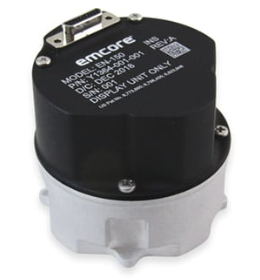
\includegraphics[height=1.3in,keepaspectratio]{figs/C/alts-pics/rlg.png}}  \\

            \multirow{2}{*}{\textit{Description and Specs}} & Micro-Electro-Mechanical Systems IMUs are small IMUs that use mechanical means to measure acceleration and rotation rates. Commonly used in lightweight applications. 
            & Fiber Optic Gyro IMUs use fiber optics to measure rotation rates. Commonly used in high-end applications
            & Ring Laser Gyro IMUs are similar to FOG IMUs but instead use lasers to measure rates of rotation.
           \\ 
            \hline
            \textit{Cost} & \$10.00-\$200.00 & \$30.00 - \$10,000.00 & \$50.00 - \$100,000.00 \\

            \multirow{3}{*}{\textit{Pros}} & \begin{itemize}
                                \item Most affordable
                                \item Small form factor
                            \end{itemize}
                        & \begin{itemize}
                            \item Very accurate
                            \item Very reliable
                            \item More stable over time than MEMS
                            \item Continuous measurements of rotation rates
                        \end{itemize}
                        
                        & \begin{itemize}
                            \item Very accurate
                            \item Very reliable
                            \item More stable over time than MEMS
                            \item Continuous measurements of rotation rates
                        \end{itemize}
                        \\
            \multirow{3}{*}{\textit{Cons}} 
                & 
                \begin{itemize}
                    \item Cheapest IMUs
                    \item Susceptible to noise and other sources of error
                    \item Require additional calibration
                \end{itemize}
                & 
                \begin{itemize}
                    \item Expensive
                    \item Larger and heavier
                    \item Requires additional cooling and other measures to remain stable
                \end{itemize}
                & 
                \begin{itemize}
                    \item Expensive
                    \item Larger and heavier
                    \item Requires additional cooling and other measures to remain stable
                \end{itemize}
                \\
            \multirow{1}{*}{\textit{Rationale}} 
                & Accurate enough, more affordable, more software libraries available.
                & Accurate, but takes much more time and effort to calibrate. Is also more expensive. 
                & Accurate, but takes much more time and effort to calibrate. Is also more expensive. 
                \\
            \hline
            \end{tabular}
            \caption{IMU Alternatives and Tradeoffs}
            \label{tab:imu}
            
        \end{table}
        
        \begin{table}[htbp]
            \centering
            \begin{tabular}{|c|p{0.18\linewidth}|>{\columncolor{orange!20}\raggedright\arraybackslash}p{0.18\linewidth}|>{\raggedright\arraybackslash}p{0.18\linewidth}|>{\raggedright\arraybackslash}p{0.18\linewidth}|}
            \hline
                 \textbf{\textit{Model}} & \textbf{Random Forest} & \textbf{Convolutional Neural Network (CNN)} & \textbf{Long Short-Term Memory (LSTM)} & \textbf{Gated Recurrent Unit (GRU)}  \\
            \hline
                 \rule{0pt}{3cm}\multirow{-3}{*}{\textit{Picture}} & \adjustbox{center}{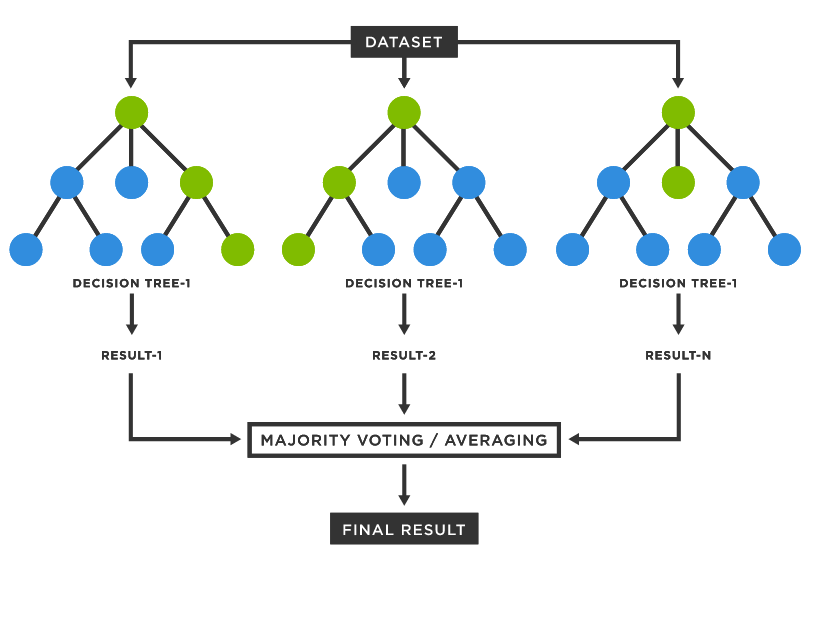
\includegraphics[height=1in, width=1.3in]{figs/C/alts-pics/random-forest.png}}& \adjustbox{center}{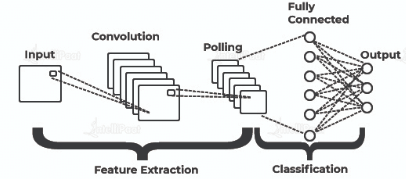
\includegraphics[height=1in, width=1.35in]{figs/C/alts-pics/cnn2.png}} & \adjustbox{center}{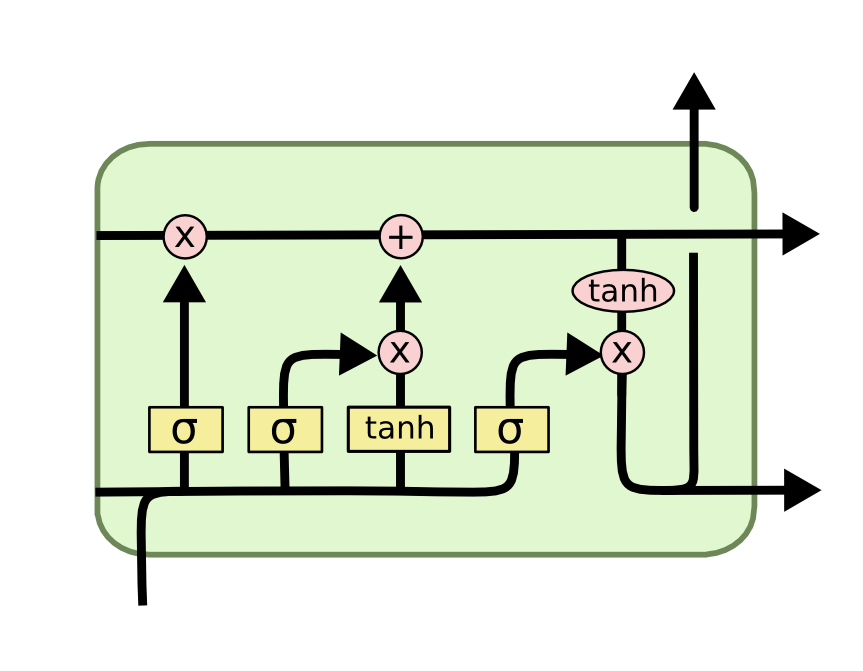
\includegraphics[height=1in]{figs/C/alts-pics/lstm.png}} & \adjustbox{center}{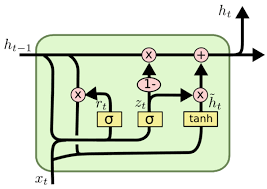
\includegraphics[height=1in]{figs/C/alts-pics/gru.png}}\\

                \multirow{2}{*}{\textit{Description and Specs}} 
                & An ensemble architecture that makes decisions based on multiple trees by splitting training data between the trees. Consists of a varying number of different architectures and chooses the best one. 
                & An architecture that divides the input data into individual pixels and performs convolutional calculations to find features. The data is subsequently fed into an MLP.
                & An evolution of an RNN that uses and input, output, and forget gate to capture long-term dependencies in input data.
                & An evolution of an RNN that uses an update and reset gate to capture long and short-term dependencies in input data. \\
            \hline

                \multirow{3}{*}{\textit{Pros}} 
                &
                \begin{itemize}
                    \item High accuracy
                    \item High variability
                    \item Most robust model
                \end{itemize}
                & 
                \begin{itemize}
                    \item Most simplistic
                    \item Good historical performance for classification of image data
                \end{itemize}
                &
                \begin{itemize}
                    \item Able to capture long term dependencies
                    \item Able to compare results from previous block and predict following blocks
                \end{itemize}
                & 
                \begin{itemize}
                    \item Able to capture long and short-term dependencies
                    \item Able to compare results from previous block and predict the following blocks
                \end{itemize}
                \\
            \multirow{3}{*}{\textit{Cons}} 
                & 
                \begin{itemize}
                    \item Highest overhead required
                    \item Most complex and computationally intense
                \end{itemize}
                & 
                \begin{itemize}
                    \item Most simplistic
                    \item Still requires a fair amount of computation power
                \end{itemize}
                & 
                \begin{itemize}
                    \item Computationally intense
                    \item Complex
                    \item Has capabilities that may not be required for this application
                \end{itemize}
                & 
                \begin{itemize}
                    \item Computationally intense
                    \item Complex
                    \item Has capabilities thay may not be required for this application
                \end{itemize}
                \\
            \multirow{2}{*}{\textit{Rationale}}
                & Requires multiple models to be trained and ran on hardware. We may not have the available processing power to quickly produce results.
                & Simple, effective, easy to work with
                & Has unneeded capabilities
                & Has unneeded capabilities
                \\
            \hline
                 
            \end{tabular}
            \caption{Machine Learning Alternatives and Tradeoffs}
            \label{tab:ml-tbl}
        \end{table}
        
        \twocolumn

\clearpage
\onecolumn
\begin{center}
    \addcontentsline{toc}{section}{Appendix D}
    \vspace*{5cm}
     {\Huge\bfseries Appendix D \par}
     \vspace{1cm}
    \textit{Preliminary Design} \\
\end{center}
\clearpage
\twocolumn

\setcounter{section}{4}
\renewcommand{\thesubsection}{D.\Alph{subsection}}
\section*{\textbf{Appendix D}}
        \setcounter{figure}{0}
        \renewcommand{\thefigure}{D.\arabic{figure}}
        \setcounter{table}{0}
        \renewcommand{\thetable}{D.\arabic{table}}
    \setcounter{subsection}{0}
    \subsection{Level 2 Block Diagram}
    The level 2 functional block diagram is shown in Fig. \ref{fig:level-2}. At the center of this system and perhaps the most crucial component is the minicomputer, the Orange Pi 5. This component is responsible for taking in data from the environment sensors, EEG cap, LCD, and rotary encoders. It has to then process that data and output the appropriate commands. The Orange Pi is also responsible for communicating with the TUL Pynq Z2 FPGA via USB, where the Orange Pi will orchestrate the machine learning of the signals and use the FPGA as a mule for the repetitive convolution calculations. 

    The Ultracortex Mark IV EEG cap will be worn by the user and will record their commands for movement. Communication between the Orange Pi and the Ultracortex will happen via Bluetooth. The incoming signal will be filtered by the processor onboard the Ultracortex and will then be passed to the Orange Pi for feature selection, classification, and any further processing that may be required. 
    
    The environmental sensors selected for this application are a combination of ultrasonic and infrared sensors. These sensors will detect obstacles in the environment through measurements of distance and give the wheelchair information about surrounding obstacles. The sensors communicate with the Orange Pi via I2C.

    The joystick module is the emergency override control of the wheelchair. As outlined previously, it will be of use to the group during testing as well as others accompanying the wheelchair user in the case of a fault in the system. The joystick will be connected to an ADC that will digitize the signal and send to the Orange Pi for processing. When the Orange Pi receives a signal from the joystick, it will halt all other commands to give the joystick the final say in controlling movement. This feature ensures that the user can take immediate control of the wheelchair if necessary and adds an extra layer of safety to the design.

    Movement will be handled by stepper motors, driven by the stepper motor controller. The controller will receive signals from the Orange Pi and transmit the appropriate movement to the stepper motors. As a measure of safety and reliability, the system is equipped with photoelectric rotary encoders. These encoders will receive the output of the position of the stepper motors and send the data to the Orange Pi. The purpose of the encoders is to provide precise feedback on the position and speed of the stepper motors. Any discrepancy detected between the desired and actual motion will be handled by a software protocol on the Orange Pi. 

    As a means of visual feedback, the system is equipped with an LCD. The screen will show a dot on an X-Y coordinate plane, and the user will be tasked with moving the dot in a particular direction to correspond to wheelchair movement.  {This display will also provide other helpful information,} such as the speed and position of the wheelchair. 

    Although the Orange Pi has been identified as the critical component of the motorized wheelchair, its operation as well as the operation of all other components is entirely dependent on a reliable power supply. The power supply unit (PSU) will provide the required power to the motor controller, FPGA, and Pi. To ensure that each of these components receives the correct voltage and current, the PSU incorporates a DC power regulator. The regulator helps to stabilize the power output by adjusting the input voltage and current to meet the requirements of each component. 
    
    \subsection{Data Flow}

    Achieving smooth and effective movement in a brain-controlled motorized wheelchair requires the integration of multiple components and the implementation of robust and reliable software protocols. This section explores the complex interplay between EEG and environmental sensor data, machine learning algorithms, and corrective inputs from the rotary encoders and manual override joystick. The flow of data through the system will be examined, from sensor input to output control signals, and how the software ensures the safe and reliable operation of the wheelchair in various scenarios.
    
        \subsubsection{Sensor and EEG}

        A flowchart of the processing of the data from the environment sensors and the EEG cap is shown in Fig. \ref{fig:eeg_and_sensor}. 
        
         \begin{figure}[htbp]
            \centering
            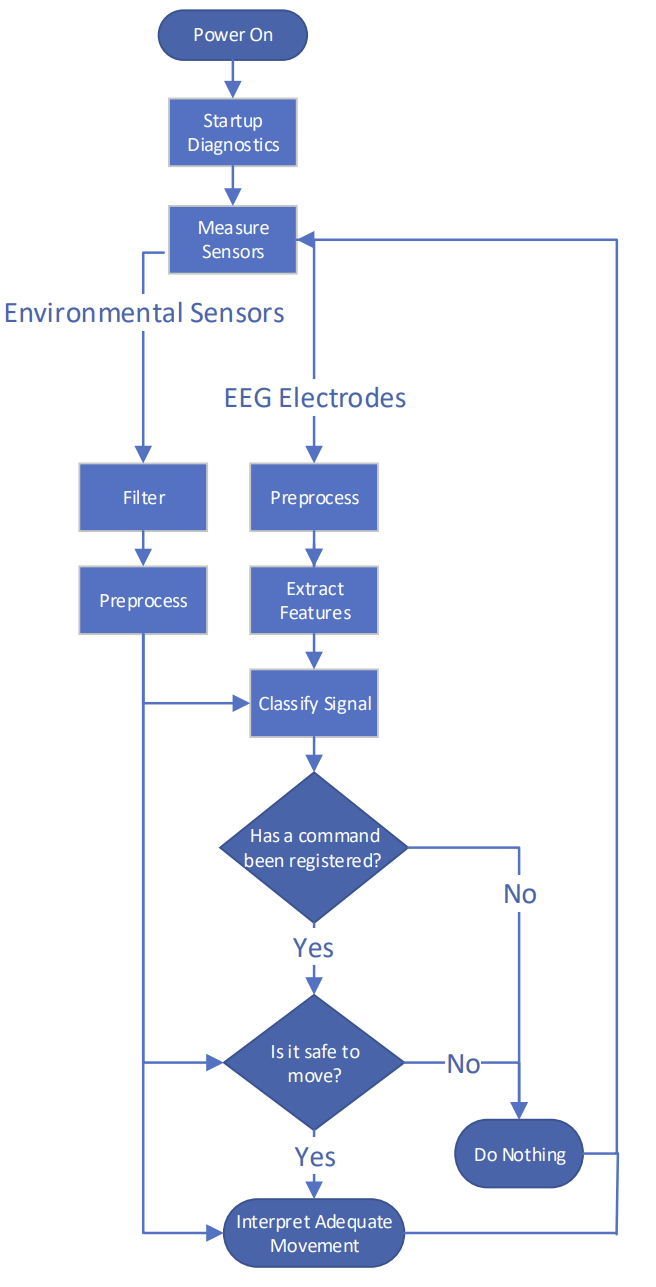
\includegraphics[height=5.1in, keepaspectratio]{figs/D/software-flowchart.png}
            \caption{EEG and Environment Sensor Flowchart}
            \label{fig:eeg_and_sensor}
        \end{figure}
            
        The two data streams follow similar flows and serve as the inputs to the machine learning model. Features such as coherence, power spectral density, and entropy will be calculated from the filtered EEG signal before they are given to the model. The sensor measurements will assist the EEG data in translating the signal into a command. This is a safety measure in the case of a false reading or similar malfunction from the EEG headset. After the model outputs a command, the sensor data will again be used to decide if the chosen direction is one that is safe. If it is determined that the chosen direction and any variation of that direction is not safe for the user, the wheelchair will do nothing. Else, the wheelchair will interpret a precise movement of the wheelchair based on both the output of the model and the surrounding obstacles. 

        \subsubsection{Machine Learning}

        In figure \ref{fig:eeg_and_sensor}, the "Classify Signal" block encapsulates the CNN algorithm used to categorize the signals into one of five commands: forward, backward, left, right, and nothing. The model is shown in Fig. \ref{fig:ml-flow}. It will be structured as a parallel CNN with a concatenation layer. 

         \begin{figure}[htbp]
            \centering
            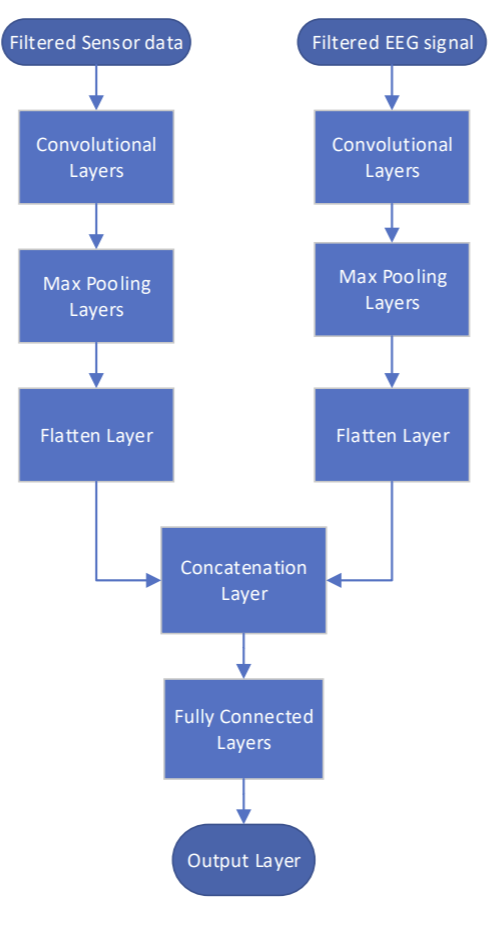
\includegraphics[height=4.7in, keepaspectratio]{figs/D/ml-flow.png}
            \caption{machine learning Data Flow}
            \label{fig:ml-flow}
        \end{figure}

        After the concatenation layer, the data will be fed into a multi-layered percepetron (MLP) containing an input layer, multiple hidden layers, and an output layer. The resulting output layer will be the weighed outputs for the five commands. 

        \subsubsection{Override and Adjustments}   
        A basic flowchart of the override and adjustment protocol in place is shown in Fig. \ref{fig:override}. This subsection of the system will be instantiated to further ensure reliable wheelchair motion. The flowchart displays the interconnection of the joystick, encoders, and motor drivers. 
         \begin{figure}[htbp]
            \centering
            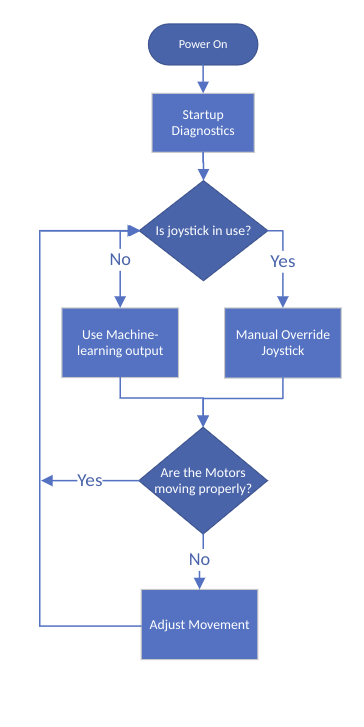
\includegraphics[height=5in, keepaspectratio]{figs/D/override.png}
            \caption{Flowchart of Adjustment and Override Protocol}
            \label{fig:override}
        \end{figure}
        
        The flowchart begins with startup diagnostics. This will detect and attempt to correct joystick drift as well as any malfunctioning of the motors or any other subsystem. Next, joystick use is checked. If no use is detected, machine learning output is used to steer the chair. If use is detected, joystick movement will be mapped to wheelchair movement. The rotary encoders will be used to check proper movement. If the motors are moving as expected, there is nothing to be done and the system loops. If the encoders detect some malfunction, then a signal will be sent to properly adjust the movement of the motors. 

    \subsection{Failure Modes and Effects Analysis}
    Through conducting an FMEA, the team was able to further explore the interconnectivity of the project and any possible associated issues. Potential points of failure that had not been previously discovered were considered, such as the event of a failing stepper motor among others. This analysis is shown in Table \ref{tab:fmea}. In this event, a braking system that can detect fault or failure would be a beneficial safety measure. Additionally, the event of the EEG headset's battery dying is very possible. To counteract this and provide a layer of transparency to the user, the team plans to include a display of the headset's battery percentage on the LCD. This analysis established the importance of having good connections between components, providing the team with valuable insights into potential failure points and how to address them.   

    \onecolumn
    \begin{figure}
        \centering
        \centerline{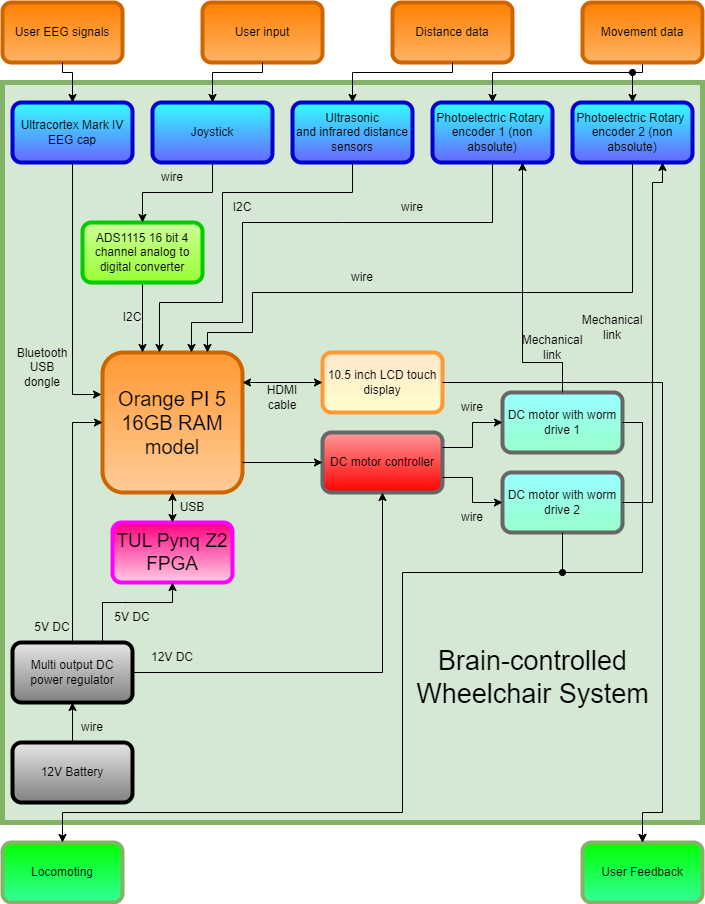
\includegraphics[height=7in, keepaspectratio]{figs/D/level_2_diagram_1.png}}
        \caption{Level 2 Functional Block Diagram}
        \label{fig:level-2}
    \end{figure}
    
    \begin{table}[htbp]
        \centering
            \begin{tabular}{|>{\columncolor{black!20}}p{0.13\linewidth}|>{\columncolor{black!5}\raggedright\arraybackslash}p{0.10\linewidth}|>{\raggedright\arraybackslash}p{0.12\linewidth}|>{\raggedright\arraybackslash}p{0.15\linewidth}|>{\raggedright\arraybackslash}p{0.15\linewidth}|>{\raggedright\arraybackslash}p{0.05\linewidth} |>{\raggedright\arraybackslash}p{0.14\linewidth}|}
            
            \hline
            \rowcolor{black!20} 
            \textit{\textbf{System}} 
            & \textbf{Components} 
            & \textbf{Failures} 
            & \textbf{Effects} 
            & \textbf{Causes} 
            & \textbf{Severity (0-5)}
            & \textbf{Solutions}\\
            \hline
             & Ultracortex Mark IV 
             & EEG cap loses communication with Orange Pi 5 
             & Wheelchair loses brain-control capability 
             & Dead battery or connection loss 
             & 5 
             & Have a fully charged backup battery on hand and always inspect headset connections before use \\
            \hhline{~------}
            & Joystick 
            & Develops Drift & Wheelchair will move in undesired directions 
            & Wear in the potentiometers 
            & 4 
            & Develop a software protocol to detect and eliminate drift \\
            % \cline{2-7}
            \hhline{~------}
            \multirow{1}{*}{\textit{System Inputs}} 
            & Environmental Sensors 
            & Calculate inaccurate distances 
            & Wheelchair will no longer be able to adjust movement or stop collisions 
            & Becomes dirty, loses connections, environmental changes 
            & 3
            & Always ensure connections are good and make sure sensors are clean \\ 
            % \cline{2-7}
            \hhline{~------}
            & Photoelectric rotary encoders 
            & Do not detect wheel movement 
            & Wheels turn due to external forces. Computer will not be able to detect and stop the wheelchair from moving 
            & Loose connections or dirty photo detector 
            & 3
            & Ensure photo detector is always clean and connections are good \\            
            \hline
            \multirow{4}{*}{\textit{Computing Systems}}
            & Orange Pi 5 
            & Computer malfunctions 
            & Wheelchair will be unresponsive or act uncontrollably 
            & Power loss, loose connections, and/or software error 
            & 4
            & Ensure power systems and all other connections are firmly connected and make sure software is up to date and working correctly \\
            % \cline{2-7}
            \hhline{~------}
            & TUL Pynq Z2 
            & Computer malfunctions 
            & EEG signals may not be interpreted correctly and stop or product undesired movement 
            & Power loss, loose or bad USB cable 
            & 4
            & Ensure software is robust, ensure physical connections are attached properly \\
            \hline 
            & Motor drivers 
            & Loss of function 
            & Wheelchair will no longer have controlled movement 
            & Power loss, power overdraw from strain, or misuse 
            & 5
            & Make sure all connections are good and power delivery system is in working order \\
            % \cline{2-7}
            \hhline{~------}
            \multirow{2}{*}{\textit{System Outputs}} 
            & DC Motors with Worm Drive 
            & Loss of function 
            & Wheelchair will not move under command and have no means of braking 
            & Power loss, power overdraw, or loose connections 
            & 5
            & Ensure motor specs, ensure secure connections \\
            % \cline{2-7}
            \hhline{~------}
            & LCD 
            & Display goes black 
            & User will not have visual indication if the chair is working and moving correctly 
            & Loose connection or misuse 
            & 3
            & Make sure the cable is connected securely and the display is secure to the chair\\
            \hline
        \end{tabular}           
        \caption{Failure Modes and Effects Analysis}
        \label{tab:fmea}
    \end{table}
    \twocolumn


%%%%%%%%%%%%%%%%%%%%%%%%%%%%%%%%%%%%%%%%%%%%%%%%%%%%%%%%%%%%
\clearpage
\onecolumn
\begin{center}
    \addcontentsline{toc}{section}{Appendix E}
    \vspace*{5cm}
     {\Huge\bfseries Appendix E \par}
     \vspace{1cm}
    \textit{Final Design} \\
\end{center}
\clearpage
\twocolumn

\setcounter{section}{5}
\renewcommand{\thesubsection}{E.\Alph{subsection}}
\section*{\textbf{Appendix E}}
        \setcounter{figure}{0}
        \renewcommand{\thefigure}{E.\arabic{figure}}
        \setcounter{table}{0}
        \renewcommand{\thetable}{E.\arabic{table}}
        \setcounter{subsection}{0}
        
    \subsection{Bill of Materials}
    The current bill of materials is displayed in Table \ref{tab:final_design_bom}, showing components that will be used to construct and implement the final design. It is worth noting that while this list covers the important parts, some additional components may be needed during the testing and building process. The wheelchair is not included in the table as the team has not yet devised an adequate plan of action to implement the design. As mentioned earlier in the report, there are some upgrades to be considered with the design involving the minicomputer. The current minicomputer, the Orange Pi 5, does not have WiFi or Bluetooth build into the motherboard, relying on external connections to achieve the functionality. The upgrade to this minicomputer, the Orange Pi 5B, has these features included on the motherboard. This will be beneficial for the implementation of the system for communication of the machine learning inputs and outputs to the remote server via WiFi and for Bluetooth communication with the Ultracortex EEG cap. 


    \begin{table}[htbp]
        \centering
        
        \begin{tabular}{|>{\raggedright\arraybackslash}p{0.30\linewidth}|>{\raggedright\arraybackslash}p{0.15\linewidth}|>{\raggedright\arraybackslash}p{0.12\linewidth}|>{\raggedright\arraybackslash}p{0.18\linewidth}|}
            
            \hline
            \rowcolor{black!20} 
            {\textbf{Part Name}} 
            & \textbf{Price} 
            & \textbf{Quantity} 
            & \textbf{Total Cost} 
            \\
            \hline

            \rowcolor{black!10}
            OpenBCI Ultracortex Mark IV & \$ 3449.99 & 1 & \$ 3449.99 \\

            \rowcolor{black!5}
            Orange Pi 5 16GB & \$ 130.99 & 1 & \$ 130.99 \\

            % \rowcolor{black!10}
            %  Standard Wheelchair & \$ 145.79 & 1 & \$ 145.79 \\


            \rowcolor{black!10}
              Roboclaw 2x7A Motor Controller & \$ 79.95 & 1 & \$ 79.95 \\

            \rowcolor{black!5}
             Ultrasonic Sensor 5 Pack & \$ 11.39 & 1 & \$ 11.39 \\

            \rowcolor{black!10}
             Infrared Sensor 6 Pack & \$ 6.99 & 1 & \$ 6.99 \\

            \rowcolor{black!5}
             Wishiot IMU-60-50 & \$ 13.99 & 1 & \$ 13.99 \\

            \rowcolor{black!10}
             Joystick & \$ 6.29 & 1 & \$ 6.29 \\

            \rowcolor{black!5}
             ADS1115 16-bit 4-channel ADC & \$ 7.99 & 1 & \$ 7.99 \\

            \rowcolor{black!10}
             Photoelectric non absolute rotary encoder 5 pack & \$ 7.29 & 1 & \$ 7.29 \\

            \rowcolor{black!5}
             12V to 5V 50W buck converter & \$ 15.99 & 1 & \$ 15.99 \\

             \rowcolor{black!10}
             12V power supply & \$ 249.98 & 1 & \$ 249.98 \\

            \rowcolor{black!5}
             Arduino RC Car Kit Base & \$ 18.99 & 1 & \$ 18.99 \\

             \rowcolor{black!10}
              RF24L01 & \$ 8.49 & 1 & \$ 8.49 \\

              \rowcolor{black!5}
              DC motor with worm drive & \$ 29.99 & 2 & \$ 59.98 \\

              \rowcolor{black!10}
              TUL Pynq Z2 FPGA & \$ 123.00 & 1 & \$ 123.00 \\

            \rowcolor{black!5}
              Orange Pi LCD Display & \$ 81.99 & 1 & \$ 81.99 \\

     
            \hline
            \rowcolor{black!20} 
            {\textbf{Within initial budget of \$7,550.00? }} 
            & \textbf{Yes} 
            & \textbf{Total} 
            & \textbf{\$ 4419.08} 
            \\
            \hline
        \end{tabular}

        \caption{Bill of Materials}
        \label{tab:final_design_bom}
    \end{table}    
    
    \subsection{Schematics}
    A schematic of the system is shown in Fig. \ref{fig:schematic}. This schematic includes all of the components mentioned in the bill of materials and displays where and how they are connected. The components include two computing modules: the Orange Pi 5 and the TUL Pynq Z2. The Orange Pi 5 acts as the conductor of the system, offloading repetitive machine learning calculations to the TUL Pynq Z2 and controlling wheelchair movement by taking in sensor and user input and outputting to the motor drivers. Both devices receive 5V power from a 12V to 5V DC buck converter.

    The remainder of the system is divided into four subsystems: environmental, locomotion, power, and user input. The environmental subsystem includes four infrared sensors, four ultrasonic sensors, and an IMU. Ultrasonic and infrared sensors communicate with the Orange Pi 5 via GPIO ports, while the IMU communicates via I2C. These sensors assist the wheelchair in making decisions about movement at two stages. The sensors serve as inputs to the machine learning model as shown in \ref{fig:eegnet} and are monitored before final output is sent to the motor drivers as shown in \ref{fig:eeg_and_sensor}. 

    The locomotion subsystem includes DC motor controllers, DC motors with worm drives, and photoelectric rotary encoders. The Orange Pi 5 communicates the desired movement to the DC motor controller via GPIO pins, which controls the speed of the motors. The motor controller uses a closed-loop system with photoelectric encoders to adjust the motor speed. The motor controller is connected to the 12V battery terminals on the motor connection side and a 5V supply on the input side. The photoelectric encoders connect to the EN1 and EN2 ports of the controller. Prior to connecting to the Orange Pi 5, the motor controller can be calibrated using the software available on the Roboclaw \cite{roboclaw} website.

    The power subsystem includes a 12V battery, 12V to 5V DC buck converter, and various cabling and adapters. The Orange Pi 5, LCD display, and TUL Pynq Z2 connect to the 5V supply of the buck converter via USB Type-C adapters. Devices that require 5V supply receive it through the V5 GPIO pins of the Orange Pi 5. Only the 12V power side of the motor controller is wired directly to the battery.

    The user input subsystem includes the OpenBCI Ultracortex Mark IV EEG cap and manual override joystick. The Ultracortex Mark IV EEG cap has its battery power supply and communicates with the Orange Pi 5 via a USB Bluetooth dongle. The manual override joystick connects to the 5V and GND GPIO pins of the Orange Pi 5. Analog signals from the joystick go into the A0 and A1 ports of an analog-to-digital ADS1115 converter that transmits joystick readings to the Orange Pi 5 via I2C. 
    
    \subsection{Software Design}
    This section will build off of what was already mentioned by earlier sections of the report, but will hone in on specific design choices where earlier sections have not gone into detail. The two sections of focus will be the specific machine learning model and the process of the startup diagnostics. 
    
    \subsubsection{Machine Learning}
    Table \ref{tab:ml-tbl} mentions the various machine learning models considered by the team after reviewing related work from \cite{a_comprehensive_review, dmtl_bci, eegnet, eegnet_processor_design, lstm_eeg, robotic_architecture, toward_brain_computer, deep_learning_eeg} and speaking with experts in both machine learning and EEG signal analysis. The team has decided to use EEGNet \cite{eegnet}, as it has been documented to perform well in applications of recognizing motor imagery commands from EEG signals, is lightweight and portable, and has been successfully implemented directly in hardware \cite{deep_learning_eeg, eegnet_processor_design}. The code for this model has also been published by the authors and is free to access on GitHub. A visualization of the network can be found in \ref{fig:eegnet}. Being a derivative of the CNN, EEGNet is comprised of convolutional layers which flatten the incoming signals that are then fed as inputs into an MLP. The model will be akin to that of what is detailed in \cite{eegnet}, however will contain the additional inputs of the environmental sensor data from the infrared sensors, ultrasonic sensors, and IMU. The network starts by deconstructing the signals into their respective frequency bands, then performs depth-wise convolution to learn frequency-specific spatial filters. This is followed by both signals undergoing separable convolution which learns a temporal summary for each feature map individually. Before being fed into the MLP, the signals are pointwise convoluted, which is a process that learns how to optimally mix the feature maps together. 
    
    \subsubsection{Startup Diagnostics}
    A finite state machine (FSM) of the startup diagnostics is shown in Fig. \ref{fig:initial_diag}. The FSM represents the software that will run upon the system being powered on and will ensure that the user input and environmental subsystems are properly functional and do not hinder wheelchair operation. Some noteworthy checks that the FSM considers are functionality of EEG electrodes, proper connection of EEG electrodes to the user's scalp, functionality of environmental sensors, and accuracy of the environmental sensors. If any of these subsystem experiences unknown behavior, then the error will be reported to the user through display on the LCD. The user will either be prompted to quickly fix the problem or if the error is severe and will not allow the wheelchair to operate safely, the system will exit. 

    \subsection{Assembly}
    The following instructions pertain to the schematic of the system and do not include details to the RC car test rig or wheelchair implementation. Refer to the schematic in Fig. \ref{fig:schematic} for more detail. 

    \begin{enumerate}
        \item Power
        \begin{itemize}
            \item Beginning with the battery, connect two wires to the positive and negative terminals each. The wires of connected to the positive terminal should be red and likewise the wires connected to the negative terminal should be black.
            \item Connect once set of red and black wires to the red and black wires of the DC buck converter and the other set of red and black wires to the battery input of the DC motor controller.
            \item From the DC buck converter attach yellow and black wires to the yellow and black wire output of the DC buck converter. This cable will have three USB type C adapters.
            \item Plug each of the USB C adapters into the USC C power port on the Orange Pi 5 and do likewise for the TUL Pynq Z2, and LCD display.
        \end{itemize}
        \item Computing
        \begin{itemize}
            \item Connect the USB cable between the Orange Pi 5 and TUL Pynq Z2
            \item Plug in the USB dongle for the Ultracortex Mark IV EEG cap.
        \end{itemize}
        \item Environmental Sensors
        \begin{itemize}
            \item Wire all the trigger wires of the four ultrasonic sensors together and connect them the proper GPIO port of the Orange Pi 5 using the schematic in Fig. \ref{fig:schematic}.
            \item Wire all the echo pins to the correct GPIO pins using the schematic as before.
            \item Connect the VCC and GND pins of each ultrasonic sensor to the 5V and GND pins of the Orange Pi 5 GPIO headers. Refer to schematic for help.
            \item For the infrared sensors, connect all the VCC and GND pins to the same 5V and GND pins of the Orange Pi 5 as you did in the previous instruction.
            \item Wire the out pin from each infrared sensor to the correct GPIO pin of the Orange Pi 5 using the schematic.
            \item Connect the VCC and GND pins of the IMU to the same as the previous set.
            \item Referring to the schematic, connect the SCL and SDA wires of the IMU to the correct GPIO pins of the Orange Pi 5.
        \end{itemize}
        \item Locomotion
        \begin{itemize}
            \item Connect the VCC and GND pins of the DC motor controller to the Correct GPIO pins of the Orange Pi 5 using the schematic.
            \item Connect the VCC and GND pins of each photoelectric encoder to the same 5V and GND connectors from the Orange Pi 5. 
            \item Connect the EN 1 and EN2 pins to the out pins of the photoelectric encoders.
            \item Connect the red wires from each motor to separate +12V screw terminals of the DC motor controller.
            \item Connect the black wires of each motor to the GND screw terminals of the DC motor controller.
        \end{itemize}
        \item User Interface
        \begin{itemize}
            \item Connect the joystick VCC and GND pins to the corresponding 5V and GND GPIO pins of the Orange Pi 5.
            \item Connect the VRX pin of the joy stick to the A0 pin and the VRY pin to A1 of the ADS1115. 
            \item Connect the VCC and GND pins to the 5V and GND GPIO pins of the Orange Pi 5.
            \item Connect the SCL and ADS pins to the same corresponding GPIO pins of the Orange Pi 5 as the IMU.
            \item Next connect the LCD display to the Orange Pi 5 using an HDMI cable.
            \item Finally, power on and put on the Ultracortex Mark IV EEG cap.
        \end{itemize}
    \end{enumerate}
    
    \subsection{Operational Gantt Chart}

    An updated Gantt chart is shown in Fig \ref{fig:updated_gantt}. The chart assigns tasks to team members and specifies the duration of their work on each task. By using this chart, the team aims to keep the remaining aspects of the project organized to maintain a consistent and productive workflow. It is the team's belief that by following this approach, the project will be completed successfully in a timely manner. 

    The team is committed to following the Operational Gantt Chart strictly in order to complete the project and allow sufficient time for testing and construction of the mock wheelchair. The team's goal is to go beyond the proof-of-concept brain-controlled RC car and to build a fully functioning wheelchair controlled by the user's thoughts. Durring the summer months, work will focus on software development and construction of the RC car testing rig. Once the rig is built, the team will continuously improve the functionality and performance of the system. When the system reaches a sufficient state, the design and construction of the wheelchair will commence. 

    \onecolumn
    \begin{figure}
        \centering
        \centerline{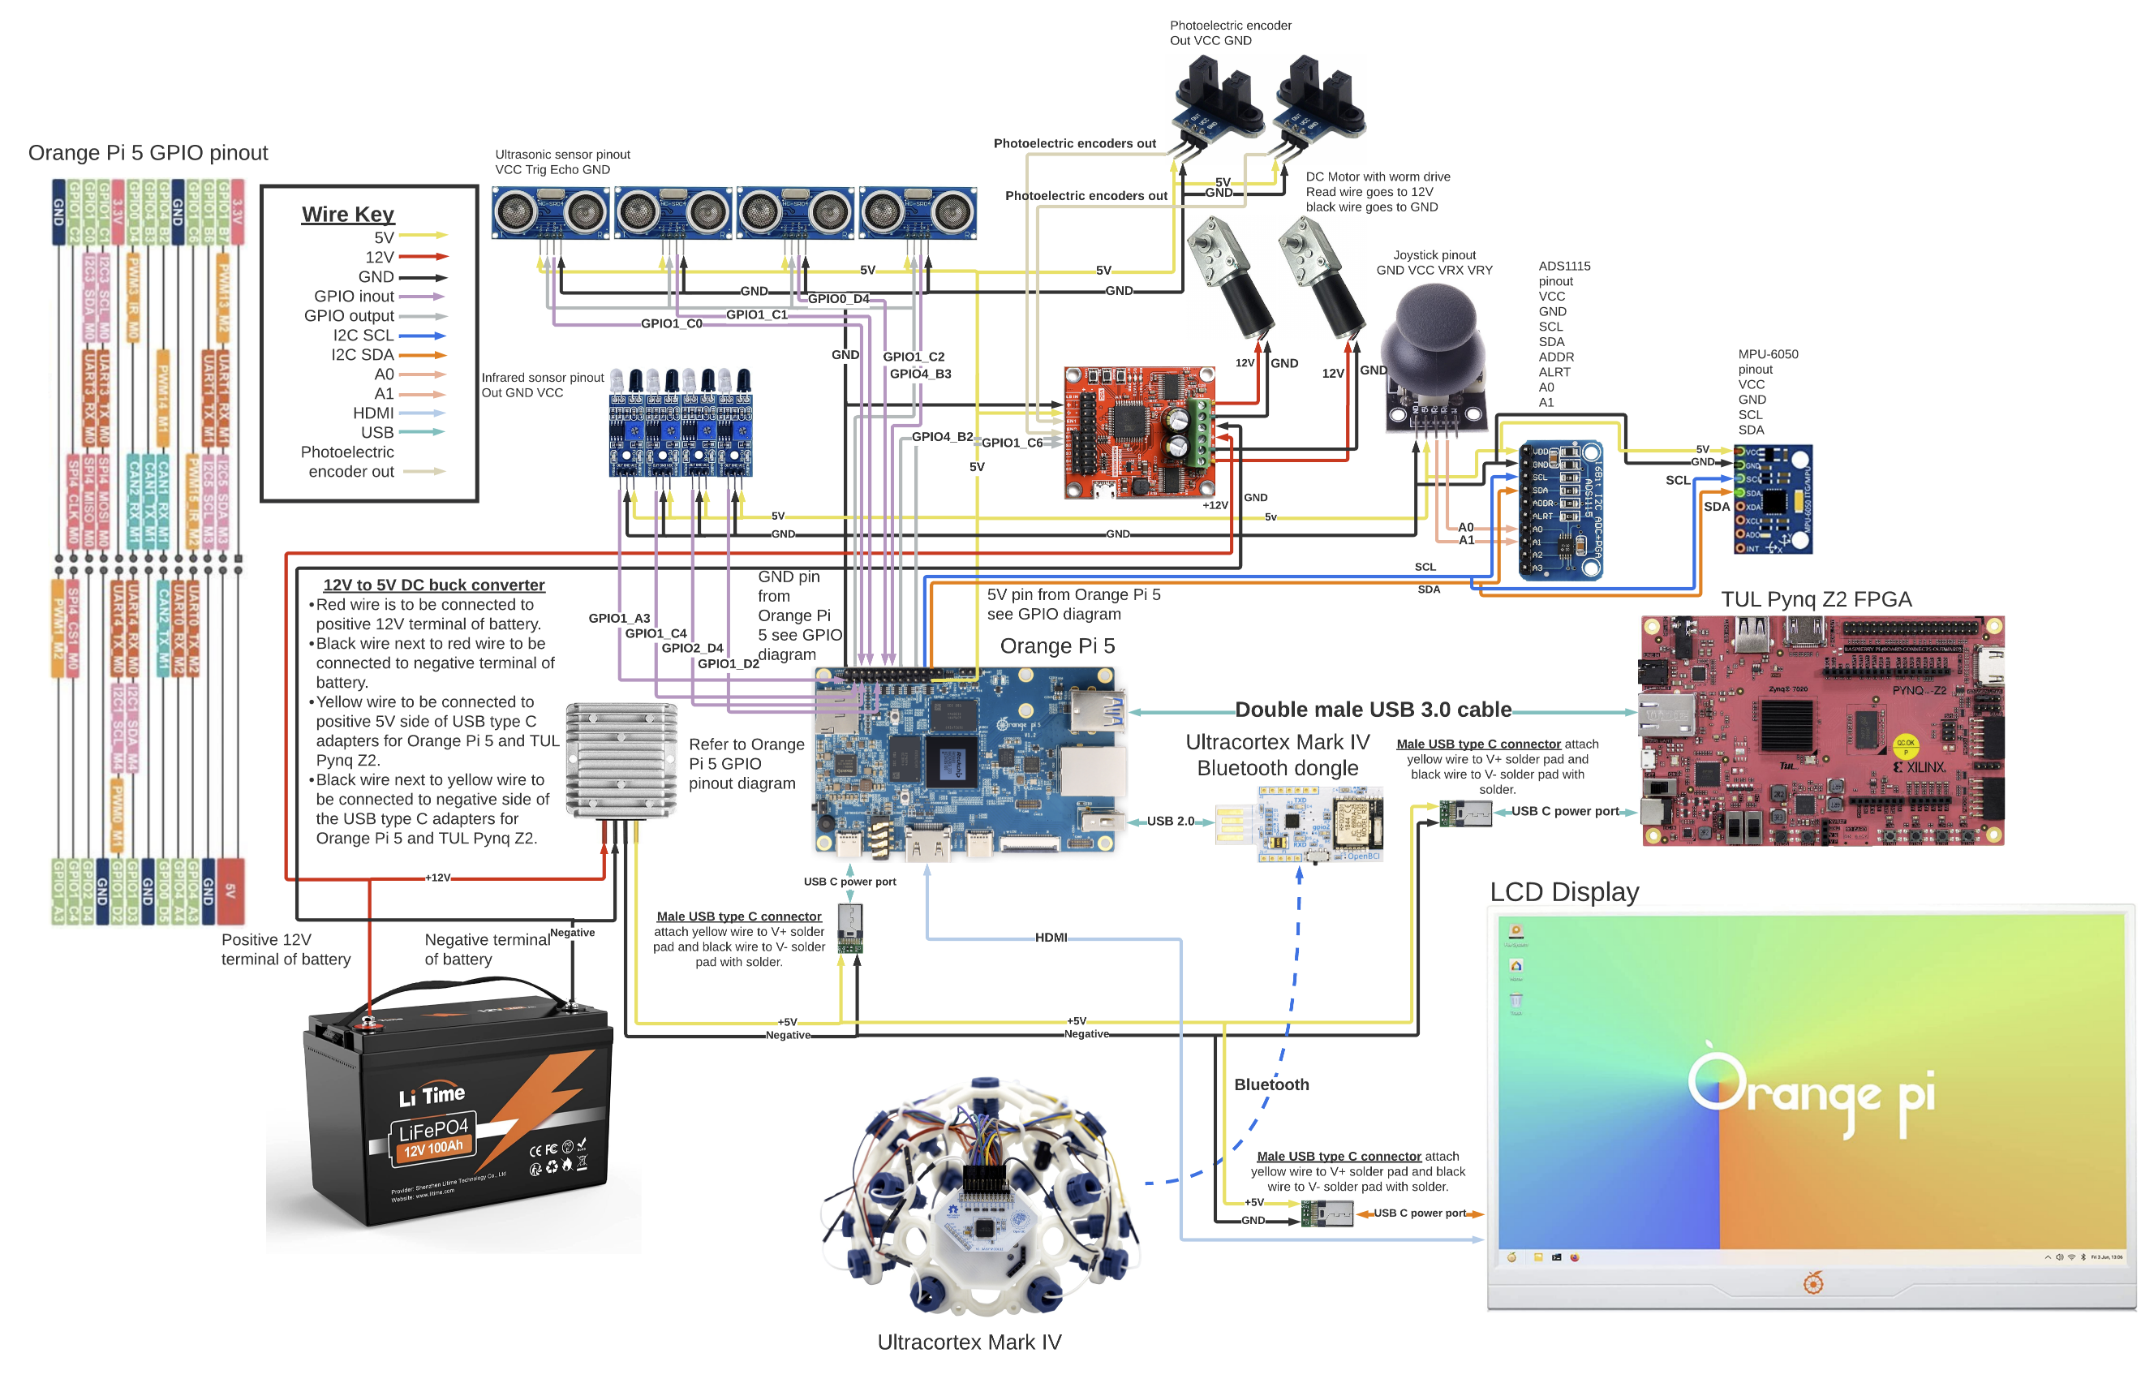
\includegraphics[angle=90,height=9in, keepaspectratio]{figs/E/schematic.png}}
        \caption{Schematic of Brain-Controlled Wheelchair}
        \label{fig:schematic}
    \end{figure}
    \twocolumn

    \onecolumn
    \begin{figure}
        \centering
        \centerline{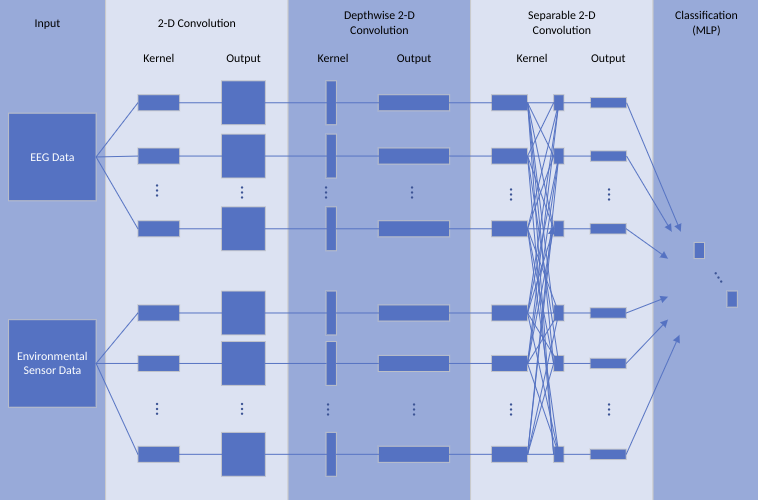
\includegraphics[height=4in, keepaspectratio]{figs/E/eegnet.png}}
        \caption{Visualization of EEGNet}
        \label{fig:eegnet}
    \end{figure}
    \begin{figure}
        \centering
        \centerline{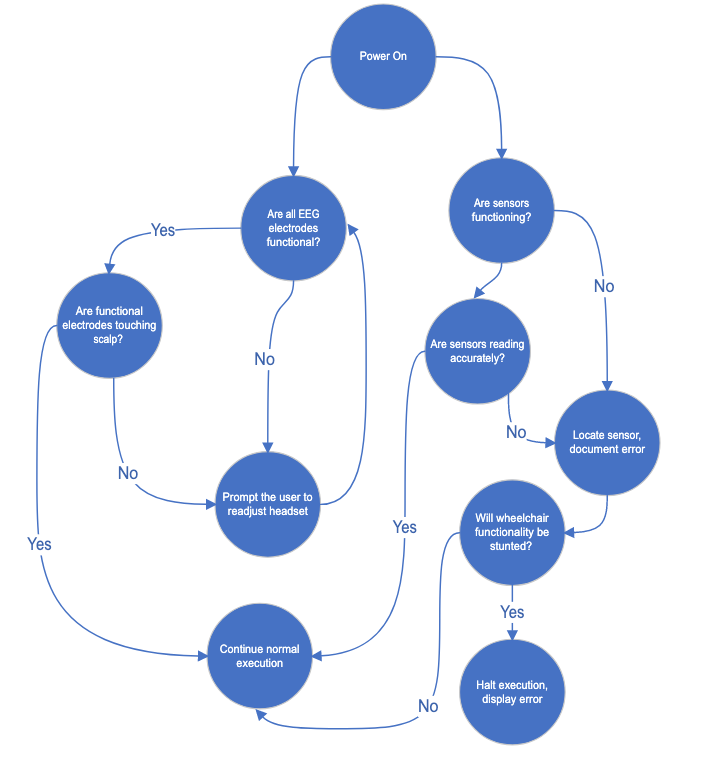
\includegraphics[height=4in, keepaspectratio]{figs/E/initial_diag_fsm.png}}
        \caption{Startup Diagnostics Finite State Machine}
        \label{fig:initial_diag}
    \end{figure}
    \twocolumn
    
    \onecolumn
    \begin{figure}
        \centering
        \centerline{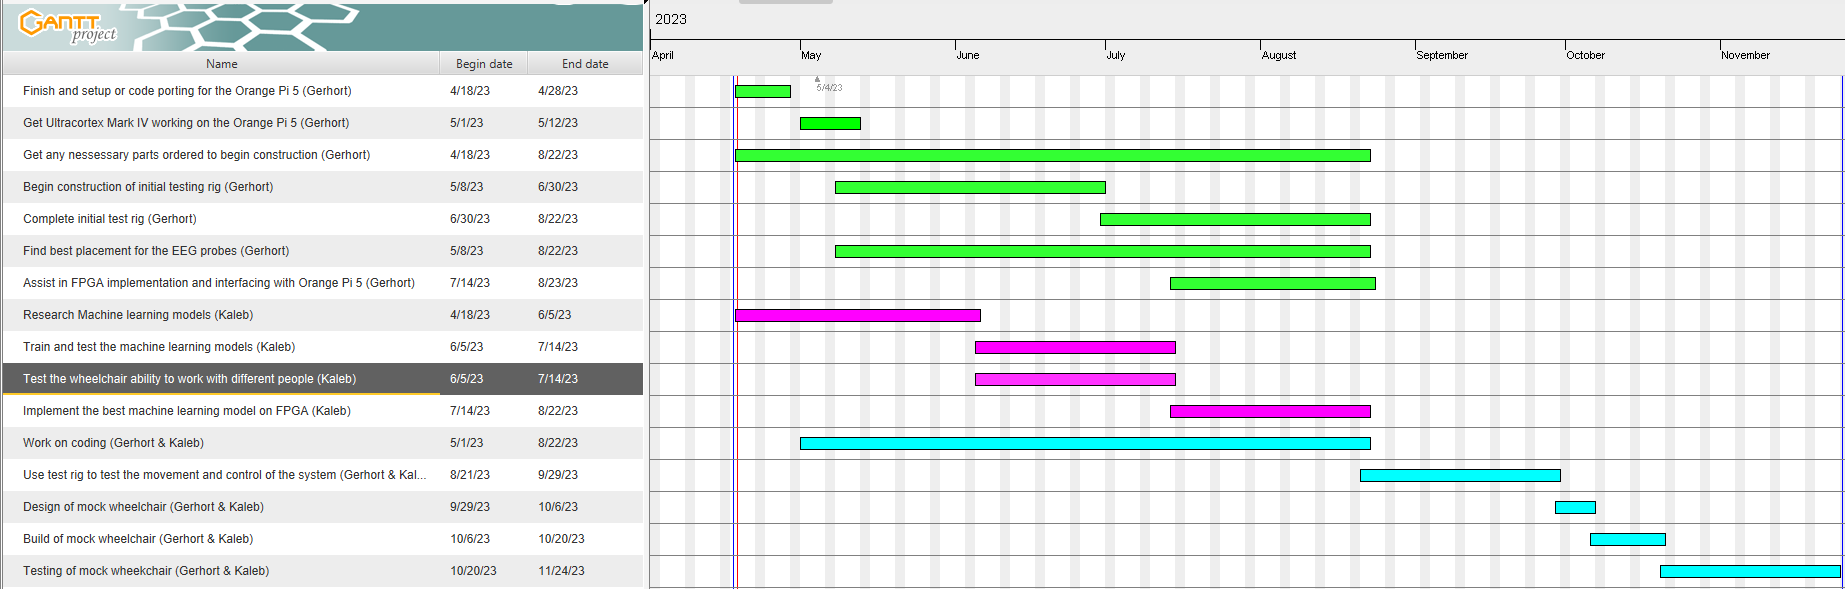
\includegraphics[angle=90,height=8.5in, keepaspectratio]{figs/E/updated_gantt.png}}
        \caption{Updated Gantt Chart}
        \label{fig:updated_gantt}
    \end{figure}
    \twocolumn

    \subsection{Server File Structure}
    The files in this project follow a specific naming convention and file structure in order to ensure that elements of this project are readily available and easy to find. The convention that the files for this project follow are outlined in Table \ref{tab:server_file_structure}.
    
    
    %% server file structure 
    \begin{table}[!ht]% [htbp]
        \centering
            \begin{tabular}{|>{}p{0.3\linewidth}|>{}p{0.35\linewidth}|>{}p{0.25\linewidth}|}
            
            \hline

             \rowcolor{black!20} \textbf{Project Name Abbreviation } &  \textbf{File Type} & \textbf{File Name}
            
            \\ \hline

            {BCW} & Assignment \newline Test Code \newline Test Results \newline Models \newline Figures \newline Weekly Reports: Gerhort \newline Weekly Reports: Kaleb & File Name

            \\ \hline

            \multicolumn{3}{|c|}{Example: BCW-Test_code-I2C.py}

            \\ \hline

        \end{tabular}           
        \caption{Server File Structure}
        \label{tab:server_file_structure}
    \end{table}

    BCW-File Server 
    
    \indent\indent Assignments 
    
    \indent\indent\indent BCW-Assignment 1.tex 
    
    \indent\indent\indent BCW-Assignment 1.pdf 
    
    \indent\indent\indent BCW-Assignment 1.pptx 
    
    \indent\indent\indent BCW-Assignment 1A.tex 

    \indent\indent\indent BCW-Assignment 1A.pdf 
    
    \indent\indent\indent BCW-Assignment 1A.pptx 
    
    \indent\indent\indent BCW-Assignment 1B.tex 
    
    \indent\indent\indent BCW-Assignment 1B.pdf 
    
    \indent\indent\indent BCW-Assignment 1B.pptx 
    
    \indent\indent\indent BCW-Assignment 1C.tex 
    
    \indent\indent\indent BCW-Assignment 1C.pdf 
    
    \indent\indent\indent BCW-Assignment 1C.pptx 
    
    \indent\indent\indent BCW-Assignment 2.tex 
    
    \indent\indent\indent BCW-Assignment 2.pdf 
    
    \indent\indent\indent BCW-Assignment 2.pptx 
    
    \indent\indent\indent BCW-Assignment 2A.tex 
    
    \indent\indent\indent BCW-Assignment 2A.pdf 
    
    \indent\indent\indent BCW-Assignment 2A.pptx 
    
    \indent\indent\indent BCW-Assignment 2B.tex 
    
    \indent\indent\indent BCW-Assignment 2B.pdf 
    
    \indent\indent\indent BCW-Assignment 2B.pptx 
    
    \indent\indent\indent BCW-Assignment 2C.tex 
    
    \indent\indent\indent BCW-Assignment 2C.pdf 
    
    \indent\indent\indent BCW-Assignment 2C.pptx 

    \indent\indent\indent BCW-Assignment 3.tex 
    
    \indent\indent\indent BCW-Assignment 3.pdf 
    
    \indent\indent\indent BCW-Assignment 3.pptx 
    
   \indent\indent Test Code 

       \indent\indent\indent BWC-Test Code-PC joystick control.py 
        
       \indent\indent\indent BWC-Test Code-PC motor driver test.py 
        
       \indent\indent\indent BWC-Test Code-PC iic test.py 
        
       \indent\indent\indent BWC-Test Code-PC MPU6050 test.py 
        
       \indent\indent\indent BWC-Test Code-PC Serial test.py 

    \indent\indent Test Results 

        \indent\indent\indent Gerhort 
        
          \indent\indent\indent\indent  BCW-Test Results-tests.doc 
            
          \indent\indent\indent\indent  BCW-Test Results-iic test.png 
            
          \indent\indent\indent\indent  BCW-Test Results-MPU6050 test.png 
            
           \indent\indent\indent\indent BCW-Test Results-motor driver test.mp4 
            
          \indent\indent\indent\indent  BCW-Test Results-maneuverability test.mp4

    \indent BCW-Test Results-motor test.mp4 

    \indent BCW-Test Results-Serial test.png 
    
    \indent BCW-Test Results-Bluetooth test.mp4 
    
    \indent Figures 
    
        \indent \indent BCW-Figure-BOM.excel 
        
        \indent \indent BCW-Figure-Gantt chart.png 
        
        \indent \indent BCW-Figure-Level 0 Diagram.png 
        
        \indent \indent BCW-Figure-Level 1 Diagram.png 
        
       \indent \indent  BCW-Figure-Level 2 Diagram.png 
        
       \indent \indent  BCW-Figure-Alternatives and trade offs.doc 
        
       \indent \indent  BCW-Figure-Objective Tree.png 
        
       \indent \indent  BCW-Figure-Operational Gantt Chart.png 
        
    \indent Models 
    
        \indent \indent BCW-Model-Motor Mount.stl 
        
        \indent \indent BCW-Model-Ultrasonic Mount.stl 
        
       \indent \indent  BCW-Model-RC wheelchair test body.stl 
        
       \indent \indent  BCW-Model-Ultracortex Mark IV ring mounts loose.stl 
        
        \indent \indent BCW-Model-Ultracortex Mark IV ring mounts loose.stl 
        
       \indent \indent BCW-Model-Ultracortex Mark IV clips.stl 
        
       \indent \indent  BCW-Model-Ultracortex Mark IV cap large whole.stl 
        
        \indent \indent BCW-Model-Ultracortex Mark IV concept cap front.stl 
        
        \indent \indent BCW-Model-Ultracortex Mark IV concept cap back.stl 
        
         
        
    \indent Weekly Reports 
    
        \indent \indent Gerhort 
        
            \indent \indent \indent Design 1 
            
               \indent \indent \indent \indent  BCW-Weekly Report-Weekly report 1.doc 
                
                \indent \indent \indent \indent BCW-Weekly Report-Weekly report 1.pdf 
                
               \indent \indent \indent \indent  BCW-Weekly Report-Weekly report 2.doc 
                
               \indent \indent \indent \indent  BCW-Weekly Report-Weekly report 2.pdf 
                
                \indent \indent \indent \indent BCW-Weekly Report-Weekly report 3.doc 
                
                \indent \indent \indent \indent BCW-Weekly Report-Weekly report 3.pdf 
                
                \indent \indent \indent \indent BCW-Weekly Report-Weekly report 4.doc 
                
               \indent \indent \indent \indent  BCW-Weekly Report-Weekly report 4.pdf 
                
                \indent \indent \indent \indent BCW-Weekly Report-Weekly report 5.doc 
                
               \indent \indent \indent \indent  BCW-Weekly Report-Weekly report 5.pdf 
                
                \indent \indent \indent \indent BCW-Weekly Report-Weekly report 6.doc 
                
                \indent \indent \indent \indent BCW-Weekly Report-Weekly report 6.pdf 
                
                \indent \indent \indent \indent BCW-Weekly Report-Weekly report 7.doc 
                
                \indent \indent \indent \indent BCW-Weekly Report-Weekly report 7.pdf 
                
            \indent \indent \indent Design 2 
            
               \indent \indent \indent \indent  BCW-Weekly Report-Weekly report 1.doc 
                
               \indent \indent \indent \indent  BCW-Weekly Report-Weekly report 1.pdf 
                
                \indent \indent \indent \indent BCW-Weekly Report-Weekly report 2.doc 
                
               \indent \indent \indent \indent  BCW-Weekly Report-Weekly report 2.pdf 
                
                \indent \indent \indent \indent BCW-Weekly Report-Weekly report 3.doc 
                
                \indent \indent \indent \indent BCW-Weekly Report-Weekly report 3.pdf 
                
                \indent \indent \indent \indent BCW-Weekly Report-Weekly report 4.doc 
                
                \indent \indent \indent \indent BCW-Weekly Report-Weekly report 4.pdf 
                
                \indent \indent \indent \indent BCW-Weekly Report-Weekly report 5.doc 
                
                \indent \indent \indent \indent BCW-Weekly Report-Weekly report 5.pdf 
                
                \indent \indent \indent \indent BCW-Weekly Report-Weekly report 6.doc 
                
                \indent \indent \indent \indent BCW-Weekly Report-Weekly report 6.pdf 
                
               \indent \indent \indent \indent  BCW-Weekly Report-Weekly report 7.doc 
                
                \indent \indent \indent \indent BCW-Weekly Report-Weekly report 7.pdf 
                
                \indent \indent \indent \indent BCW-Weekly Report-Weekly report 8.doc 
                
               \indent \indent \indent \indent  BCW-Weekly Report-Weekly report 8.pdf 
                
        \indent \indent Kaleb 
        
            \indent \indent \indent Design 1 
            
                \indent \indent \indent \indent  BCW-Weekly Report-Weekly report 1.doc 
                
                \indent \indent \indent \indent BCW-Weekly Report-Weekly report 1.pdf 
                
               \indent \indent \indent \indent  BCW-Weekly Report-Weekly report 2.doc 
                
               \indent \indent \indent \indent  BCW-Weekly Report-Weekly report 2.pdf 
                
                \indent \indent \indent \indent BCW-Weekly Report-Weekly report 3.doc 
                
                \indent \indent \indent \indent BCW-Weekly Report-Weekly report 3.pdf 
                
                \indent \indent \indent \indent BCW-Weekly Report-Weekly report 4.doc 
                
               \indent \indent \indent \indent  BCW-Weekly Report-Weekly report 4.pdf 
                
                \indent \indent \indent \indent BCW-Weekly Report-Weekly report 5.doc 
                
               \indent \indent \indent \indent  BCW-Weekly Report-Weekly report 5.pdf 
                
                \indent \indent \indent \indent BCW-Weekly Report-Weekly report 6.doc 
                
                \indent \indent \indent \indent BCW-Weekly Report-Weekly report 6.pdf 
                
                \indent \indent \indent \indent BCW-Weekly Report-Weekly report 7.doc 
                
                \indent \indent \indent \indent BCW-Weekly Report-Weekly report 7.pdf 
                
            \indent \indent \indent Design 2 
            
               \indent \indent \indent \indent  BCW-Weekly Report-Weekly report 1.doc 
                
               \indent \indent \indent \indent  BCW-Weekly Report-Weekly report 1.pdf 
                
                \indent \indent \indent \indent BCW-Weekly Report-Weekly report 2.doc 
                
               \indent \indent \indent \indent  BCW-Weekly Report-Weekly report 2.pdf 
                
                \indent \indent \indent \indent BCW-Weekly Report-Weekly report 3.doc 
                
                \indent \indent \indent \indent BCW-Weekly Report-Weekly report 3.pdf 
                
                \indent \indent \indent \indent BCW-Weekly Report-Weekly report 4.doc 
                
                \indent \indent \indent \indent BCW-Weekly Report-Weekly report 4.pdf 
                
                \indent \indent \indent \indent BCW-Weekly Report-Weekly report 5.doc 
                
                \indent \indent \indent \indent BCW-Weekly Report-Weekly report 5.pdf 
                
                \indent \indent \indent \indent BCW-Weekly Report-Weekly report 6.doc 
                
                \indent \indent \indent \indent BCW-Weekly Report-Weekly report 6.pdf 
                
               \indent \indent \indent \indent  BCW-Weekly Report-Weekly report 7.doc 
                
                \indent \indent \indent \indent BCW-Weekly Report-Weekly report 7.pdf 
                
                \indent \indent \indent \indent BCW-Weekly Report-Weekly report 8.doc 
                
               \indent \indent \indent \indent  BCW-Weekly Report-Weekly report 8.pdf 
    

%%%%%%%%%%%%%%%%%%%%%%%%%%%%%%%%%%%%%%%%%%%%%%%%%%%%%%%%%%%%
\clearpage
\onecolumn
\begin{center}
    \addcontentsline{toc}{section}{Appendix F}
    \vspace*{5cm}
     {\Huge\bfseries Appendix F \par}
     \vspace{1cm}
    \textit{Testing Plan} \\
\end{center}
\clearpage
\twocolumn

\setcounter{section}{6}
\renewcommand{\thesubsection}{F.\Alph{subsection}}
\section*{\textbf{Appendix F}}
        \setcounter{figure}{0}
        \renewcommand{\thefigure}{F.\arabic{figure}}
        \setcounter{table}{0}
        \renewcommand{\thetable}{F.\arabic{table}}
        \setcounter{subsection}{0}
        
    \subsection{Testing Plan}
   To thoroughly test the entirety of the Brain-Controlled Wheelchair, the system is divided into subassemblies and subsystems as shown in Fig \ref{fig:testing_plan} in the form of a Preliminary Comprehensive Modular Build and Testing Plan (P-CMBTP). Each subsystem contains component level tests to ensure a quality and reliable build. The two subassemblies which encapsulate the scope of this project are the RC Wheelchair Subassembly and the Brain Control Subassembly. Tests will be conducted to measure the capabilities of both the hardware and software of the system. This section outlines the nature of the planned tests for each of the components in the leaves of the P-CMBTP.  
        
        \subsubsection{Motor Driver: 0.1.1.1}
        This test will serve to check the ability of the motor driver to perform the required functions needed for the RC wheelchair subassembly to work properly. The functions that will be test are at what duty cycle will the motors start to turn in both directions, current draw under normal speeds, and current draw under a worst-case scenario. This test will inadvertently test the motors as well for the same functions.

        \subsubsection{Motors: 0.1.1.2}
         A test will be conducted to check the functionality of the DC motors used for locomotion of the RC wheelchair. The test results from the motor driver test will be taken into account after along with the results of this test. This test will work by driving the RC wheelchair for a duration of twenty minutes while preforming maneuvers quick forward to reverse, turning, and full speed. The motors will be check for over heating along with visual inspection of the motors ability to perform the tasks mentioned.

        \subsubsection{Wheels: 0.1.1.3}
       Two factors concerning the wheels of the RC wheelchair will be tested. Those factors are traction and smoothness of rotation. Traction tests consist of preforming quick motions such as abrupt stopping, full speed forward and reverse, shar turns, and wide turns. It will be visually inspected with a team member if the wheels did not provide enough traction or do not have smooth rotation. 

        \subsubsection{Straight Line: 0.1.1.4}
        It is imperative that when the command to go forward is sent to the wheelchair, that the wheelchair actually goes forward. This test is design to measure the ability of the RC Wheelchair to go 2 meters in a straight line with a deviation to either side of less than three inches. 

        \subsubsection{90\textdegree Turn: 0.1.1.5}
        This test measures the ability of the wheelchair to make a 90 degree turn in a finite amount of time given a certain number of commands received from the PC application. 
        
        \subsubsection{UART: 0.1.2.1}
        One UART port will be required for the CH-05 Bluetooth module to function. Movement commands along with warning signals from the wheelchair will be sent and received through this UART port. The focus of this test is to verify the ability of UART to receive signals on the Pi Pico from the multiple sensors. Tests will consist of verifying the information received on the Pi Pico from the sensors through connecting the Pi Pico directly to the PC, thus circumventing the use of Bluetooth. 


        \subsubsection{I2C: 0.1.2.2}
        One device in the Brain-controlled wheelchair system uses I2C communication. This test will simply serve to ensure the I2C communication between the MPU6050 and Pi Pico is in working order. Reliability will be tested by turning the RC wheelchair subassembly on and off and verify that the Pi Pico is still able to communicate to the MPU through I2C and receive the required data. 

        \subsubsection{Bluetooth: 0.1.2.3}
        This test serves to ensure a Bluetooth connection between a PC and the RC wheelchair subassembly. This test will simply consist of checking if a PC can connect to the CH-05 Bluetooth module and communicate bidirectionally with the device. Range will also be tested by driving the RC wheelchair down a long hallway and measuring the distance at which it loses communication. 

        \subsubsection{Ultrasonic: 0.1.3.1}
        The purpose of this test will be to determine how well the ultrasonic sensors can help prevent crashes. The test will consist of purposely trying to crash the RC wheelchair into a wall or other obstacles. 

        \subsubsection{MPU6050: 0.1.3.2}
        IIn this test one main function of the MPU will be tested. That function is the ability of the MPU6050 to tell which way is down by measuring the acceleration due to gravity. This test may consist of position the MPU6050 in different orientation and check if it can correctly tell which way is down no matter which how the MPU is positioned. The test will also check the MPU6050 software ability to filter out the noise of the RC wheelchair accelerating. This will be tested by moving the module from a resting spot at the speed of the RC wheelchair and checking if false warning appear.

        \subsubsection{Structural Integrity: 0.1.4.1}
        This test serves to check the strength of the frame of the RC wheelchair subassembly. Testing will involve the ability of the wheelchair subassembly to withstand collisions or impacts. 
        
        \subsubsection{Ergonomic Mobility: 0.1.4.2}
       This test will be conducted when the RC wheelchair subassembly is near completion. The goal of this test will be how the RC wheelchair subassembly imitates the behavior of a real motorized wheelchair. This will consist of ensuring the smooth and comfortable operation of the wheelchair under normal use conditions.

        \subsubsection{User Friendlieness: 0.2.1.1}
        The user friendliness test aims to determine how well a new user can use the system with little outside explanation. This test will consist of gathering subjects who have not been exposed to the user interface and testing their ability to navigate the software with little to no guidance. Passing this test involves a majority of users who are able to easily and smoothly operate the system through the user interface.

        \subsubsection{Performance: 0.2.1.2}
        This test will serve to check how easily the User interface subassembly can run on a computer. Test will consist of measuring RAM, processor utilization, and GPU utilization is required to run the User interface subassembly. 

        \subsubsection{User Profile Creation: 0.2.1.3}
        A test will be conducted to check how well the new user adaptability subsystem can create a new profile for controlling the RC wheelchair catered to their EEG signals. Testing may involve check if the profiles are uniquely different between several users or different from a default. This test may also involve how well after creating a user profile the user can operate the wheelchair.

        \subsubsection{Save / Load Profiles: 0.2.1.4}
        This test serves to check how well the PC application can save and load a user RC wheelchair control profile. Testing may involve getting a user to make a profile closing the application and reopening it to see if the profile was saved. 

        \subsubsection{Headset Connection: 0.2.2.1}
        Test ensures that the onboard PCB on the headset can connect and maintain connection to the PC through the dongle and in the code 

        \subsubsection{Obtain EEG Data: 0.2.2.2}
        Test ensures that data can be received from the EEG headset

        \subsubsection{Read/Write Data from file: 0.2.2.3}
        Test ensures that data received from the headset can be outputted to a file. This test also ensures that the file can be read from and appended to. 

        \subsubsection{Format Data and Train Model: 0.2.2.4}
        This test ensures that the received data from the headset can be formatted in a way that our machine learning model can be fit to. This test also ensures that the model can be saved to an H5 file and that the model can be loaded back into the code.

        \subsubsection{Generate Predictions from Incoming Data: 0.2.2.5}
        This test ensures that live EEG data can be used to generate predictions from a trained model.
        
        \subsubsection{Machine Learning Accuracy: 0.2.3.1}
        The most crucial component of the system as a whole is being able to correctly classify a user's EEG signals into their desired movement commands. The accuracy of the machine learning model is dependent on many factors, but tests under 0.2.3.1 will hone in on the nature of the incoming EEG signal. Tests will involve using different categories of neural signals to get the best accuracy for a given machine learning model. These categories of signals include MI and P300. 

        \subsubsection{Hyperparameter Tuning: 0.2.3.1.0}
        The machine learning model of choice, EEGNet, has numerous hyperparameters that can be changed which result in a slightly different machine learning model which processes the data. Depending on the values of these hyperparameters will change the accuracy of the classification. 

        \subsubsection{Moving Average Filter: Training Data: 0.2.3.1.1}
        The quality of a machine learning model depends on the quality of the incoming data. In order to generate more predictions in a shorter amount of time, a type of moving average filter will be applied to the incoming data. This means that, rather than generate predictions from an entirely new subset's worth of data, predictions will be generated from only a small amount of new data, but mostly data used from the previous prediction. This test determines whether splitting the training data for this application is beneficial or detrimental. 

        \subsubsection{Moving Average Filter: Testing Data: 0.2.3.1.2}
        This test determines the effect of the moving average filter applied to the testing data. This test will measure the effect of applying the moving average filter to only the testing data. 

        \subsubsection{EEG Signal Filtration: 0.2.3.1.3}
        The downfall of non-invasive BCIs are the noise that often plague EEG signals. Tests will be conducted to calculate signal-to-noise (SNR) ratios on the data from the active electrodes. This test will be highly dependent on the conditions of the surrounding environment. Tests will be conducted while the user is in different states of movement to imitate the movement of a wheelchair.

        \subsubsection{EEG Signal Denoising: 0.2.3.1.4}
        This test will use techniques included in the brainflow library to remove noise from the EEG signals from the UltraCortex Mark IV. The denoised signals will then be sent through our model to determine if this is an effective method of improving the model accuracy. 
        
        \subsubsection{Electrode Placement: 0.2.3.2}
        This test will serve to help find the best general placement of electrodes around a users head. Locations that are supported for use in similar BCI systems in the literature will serve as a foundation for these tests.  
        
     

    \onecolumn
    \begin{figure}[htbp]
            \centerline{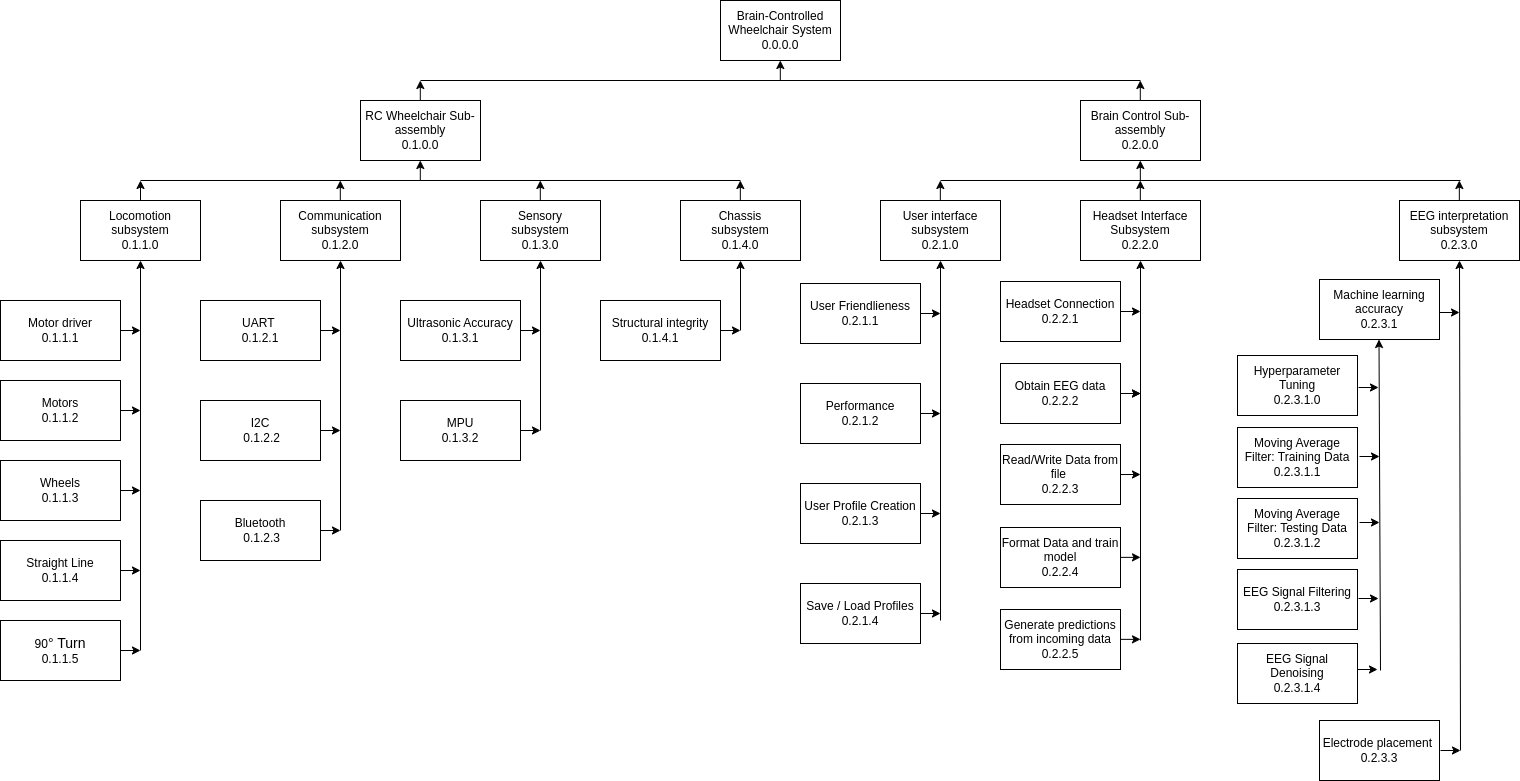
\includegraphics[height=5in,keepaspectratio, angle=90]{figs/F/testing_tree.png}}
            \caption{P-CMBTP}
            \label{fig:testing_plan}
        \end{figure}    
    \twocolumn
        
    \subsection{Test Report Example Template}
    Table \ref{tab:test_report_template} shows a test report sample that will be included for each of the leaves on the Modular Build Plan Testing Tree. This template will be altered slightly for each test depending on the nature and results of the test, however the core structure will remain the same. 

    % \onecolumn
    \renewcommand{\arraystretch}{1.5}
        \setlength{\arrayrulewidth}{1.25pt}

    %%%%%%%
    % EXAMPLE TEST REPORT
    \begin{table}[!ht]% [htbp]
        \centering
            \begin{tabular}{|>{\columncolor{black!5}}p{0.25\linewidth}|>{}p{0.65\linewidth}|}
            
            \hline
            \rowcolor{black!20} 
             \multicolumn{2}{|c|}{\textbf{Test Report - Leaf on the Tree - Format}} % & \textbf{Header} \\ % Header row with one merged cell and one regular cell
            \\ \hline

            \textit{Title of Test: } & .. 
            
            \\ \hline

            \textit{Date:} & ..

            \\ \hline

            \textit{Person(s) Conducting:} & ..

            \\ \hline

            \textit{Signature / Witness:} & ..

            \\ \hline

            \textit{Purpose:} & .. 

            \\ \hline

            \textit{Device Under Test:} & ..

            \\ \hline

            \textit{Equipment Settings and Software Used to test:} & .. 

            \\ \hline

            \textit{Experiment Procedure:} & ..

            \\ \hline 

            \textit{Hardware / Software Diagram: } & .. 

            \\ \hline 

            \textit{Data:} & .. 

            \\ \hline 

            \textit{Integration:} & ..

            \\ \hline

            \textit{Root Cause Analysis: } & ..

            \\ \hline

            \textit{Recommended Modifications: } & .. 

            \\ \hline

        \end{tabular}           
        \caption{Test Report Example Template}
        \label{tab:test_report_template}
    \end{table}

    \newpage
    \subsection{Completed Tests}
    This section includes tables of completed tests as well as discussions on the success and failures of the tests where needed. 

    \begin{figure}[htbp]
            \centerline{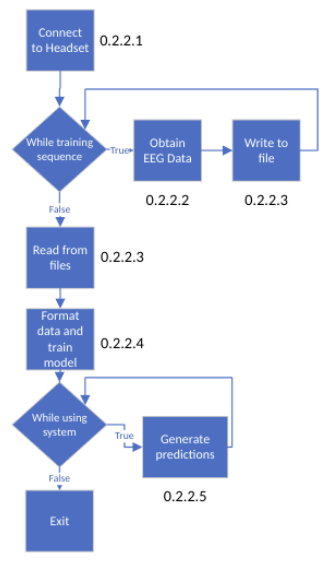
\includegraphics[height=5in,keepaspectratio]{figs/F/0.2.2_flowchart.png}}
            \caption{Flowchart of Subsystem 0.2.2.0}
            \label{fig:0.2.2.0_flowchart}
        \end{figure} 

    %0.2.2.1
    \begin{table}[!ht]% [htbp]
        \centering
            \begin{tabular}{|>{\columncolor{black!5}}p{0.25\linewidth}|>{}p{0.65\linewidth}|}
            
            \hline
            \rowcolor{black!20} 
             \multicolumn{2}{|c|}{\textbf{Test Report - 0.2.2.1 - Headset Connectivity}} % & \textbf{Header} \\ % Header row with one merged cell and one regular cell
            \\ \hline

            \textit{Title of Test: } & Connect to EEG Headset
            
            \\ \hline

            \textit{Date:} & 10/07/2023

            \\ \hline

            \textit{Person(s) Conducting:} & Kaleb Guillot

            \\ \hline

            \textit{Signature / Witness:} & Gerhort Alford

            \\ \hline

            \textit{Purpose:} & This test ensures that a connection between the board and computer can be established and maintained for five seconds. This test makes the connection in code written by the team rather than using the user interface by OpenBCI.

            \\ \hline

            \textit{Device Under Test:} & Cyton Daisy Board and Dongle

            \\ \hline

            \textit{Equipment Settings and Software Used to test:} & Plug in the dongle to the PC, and make sure the switch on the onboard processor on the headset is set to ‘PC’. Important note: when connecting for the first time on Linux computers, access to the usb port has to be granted with the following lines in the terminal: \newline  
            \$  sudo usermod -aG dialout \$USER\newline 
            \$ sudo chmod a+rw /dev/ttyUSB0\newline
            Link to file: {\url{https://github.com/kguilly/BrainControlledWheelchair/blob/main/EEG_ML/tests/TST_0.2.2.1.py}}

            \\ \hline

            \textit{Experiment Procedure:} & Establish connection to the headset, wait 5 seconds, release the connection. If the connection is not broken, the test was a success 

            \\ \hline 

            \textit{Integration:} & Refer to Fig. \ref{fig:0.2.2.0_flowchart}

            \\ \hline  
            
            % \textit{Validation} & This test was repeated 5 times across 4 machines spanning 4 different operating systems: Windows 10 Pro, Windows 11, Linux Mint, Zorin. All were successful  

            % \\ \hline
             
        \end{tabular}           
        \caption{Headset Connection Test}
        \label{tab:test_report_template}
    \end{table}

    % 0.2.2.2
    \begin{table}[!ht]% [htbp]
        \centering
            \begin{tabular}{|>{\columncolor{black!5}}p{0.25\linewidth}|>{}p{0.65\linewidth}|}
            
            \hline
            \rowcolor{black!20} 
             \multicolumn{2}{|c|}{\textbf{Test Report - 0.2.2.2 - Obtain EEg Data}} 
             
            \\ \hline

            \textit{Title of Test: } & Obtain EEG data from Ultracortex 
            
            \\ \hline

            \textit{Date:} & 10.20.2023

            \\ \hline

            \textit{Person(s) Conducting:} & Kaleb Guillot

            \\ \hline

            \textit{Signature / Witness:} & Gerhort Alford

            \\ \hline

            \textit{Purpose:} & This test takes 0.2.2.1 a step further streams data from the connected headset and prints the data. This ensures that data is actually being received in the manner that is expected.  

            \\ \hline

            \textit{Device Under Test:} & Cyton Daisy Board and Dongle

            \\ \hline

            \textit{Equipment Settings and Software Used to test:} & Plug in the dongle to the PC, and make sure the switch on the onboard processor on the headset is set to ‘PC’. Ensure access to usb port is enabled on your machine Link to test file: {\url{https://github.com/kguilly/BrainControlledWheelchair/blob/main/EEG_ML/tests/TST_0.2.2.2.py }} 

            \\ \hline

            \textit{Experiment Procedure:} & Maintain connection for 5 seconds, take 5 seconds worth of data from the buffer and print it out.  

            \\ \hline 

            % \textit{Hardware / Software Diagram: } & .. 

            % \\ \hline 

            \textit{Data:} & Fig. \ref{fig:0.2.2.2_output} displays a picture of the output from a run of this test. 

            \\ \hline 

            \textit{Integration:} & Refer to fig \ref{fig:0.2.2.0_flowchart}

            \\ \hline

            % \textit{Validation: } & This test was repeated 5 times across 4 machines spanning 4 different operating systems: Windows 10 Pro, Windows 11, Linux Mint, Zorin. All were successful  

            % \\ \hline
             
        \end{tabular}           
        \caption{Obtain EEG Data Test}
        \label{tab:obtain_eeg_data}
    \end{table}
    \onecolumn
    \begin{figure}[htbp]
            \centerline{\includegraphics[height=4in,keepaspectratio, angle = 90]{figs/F/0.2.2.2_output.png}}
            \caption{Sample output from 0.2.2.2}
            \label{fig:0.2.2.2_output}
        \end{figure} 
    \twocolumn

    % 0.2.2.3
    \begin{table}[!ht]% [htbp]
        \centering
            \begin{tabular}{|>{\columncolor{black!5}}p{0.25\linewidth}|>{}p{0.65\linewidth}|}
            
            \hline
            \rowcolor{black!20} 
             \multicolumn{2}{|c|}{\textbf{Test Report - 0.2.2.3 - Read / Write EEG Data}} % & \textbf{Header} \\ % Header row with one merged cell and one regular cell
            \\ \hline

            \textit{Title of Test: } & Read and Write headset data to and from files 
            
            \\ \hline

            \textit{Date:} & 10.20.2023

            \\ \hline

            \textit{Person(s) Conducting:} & Kaleb Guillot

            \\ \hline

            \textit{Signature / Witness:} & Gerhort Alford 

            \\ \hline

            \textit{Purpose:} & This test ensures that the headset’s data can be written to a file, and that data can be reliably read from a file in a format that is usable. This test also ensures that new data from the headset is appended to the end of the file and the data is not overwritten.  

            \\ \hline

            \textit{Device Under Test:} & Cyton Daisy Board and Dongle

            \\ \hline

            \textit{Equipment Settings and Software Used to test:} & Plug in the dongle to the PC, and make sure the switch on the onboard processor on the headset is set to ‘PC’. Ensure access to usb port is enabled on your machine. Link: {\url{https://github.com/kguilly/BrainControlledWheelchair/blob/main/EEG_ML/tests/TST_0.2.2.3.py }} 

            \\ \hline

            \textit{Experiment Procedure:} & This test takes 0.2.2.2 a step further. It gathers the data after five seconds and rather than printing the data out, the data is saved to a file. The file is then loaded, and the tail end is printed. Then, five more seconds of headset data is written to the end of the file. The file is again loaded into a dataframe, and the tail is printed out. 

            \\ \hline 

            % \textit{Hardware / Software Diagram: } & .. 

            % \\ \hline 

            \textit{Data:} & Link: {\url{https://github.com/kguilly/BrainControlledWheelchair/blob/main/EEG_ML/tests/test_data/0.2.2.3.csv }}

            \\ \hline 

            \textit{Integration:} & Refer to Fig. \ref{fig:0.2.2.0_flowchart}

            % \\ \hline

            % \textit{Validation: } & This test was repeated 5 times across 4 machines spanning 4 different operating systems: Windows 10 Pro, Windows 11, Linux Mint, Zorin. All were successful.

            \\ \hline
        \end{tabular}           
        \caption{Read / Write EEG Data Test}
        \label{tab:0.2.2.3_testtable}
    \end{table}

    % 0.2.2.4
    \begin{table}[!ht]% [htbp]
        \centering
            \begin{tabular}{|>{\columncolor{black!5}}p{0.25\linewidth}|>{}p{0.65\linewidth}|}
            
            \hline
            \rowcolor{black!20} 
             \multicolumn{2}{|c|}{\textbf{Test Report - 0.2.2.4 - Format Data and Train Model}} % & \textbf{Header} \\ % Header row with one merged cell and one regular cell
            \\ \hline

            \textit{Title of Test: } & Format EEG data and train machine learning model  
            
            \\ \hline

            \textit{Date:} & 10.20.2023 

            \\ \hline

            \textit{Person(s) Conducting:} & Kaleb Guillot 

            \\ \hline

            \textit{Signature / Witness:} & Gerhort Alford 

            \\ \hline

            \textit{Purpose:} & This test ensures that the EEG data stored in the files from training can be formatted in a manner that the machine learning model needs, and that model can then be trained with that data. This test also ensures that the model can be save to an H5 file for later use in generating predictions or training further.   

            \\ \hline

            \textit{Device Under Test:} & Cyton Daisy Board and Dongle 

            \\ \hline

            \textit{Equipment Settings and Software Used to test:} & Plug in the dongle to the PC, and make sure the switch on the onboard processor on the headset is set to ‘PC’. Ensure access to usb port is enabled on your machine. Link to test file: {\url{https://github.com/kguilly/BrainControlledWheelchair/blob/main/EEG_ML/tests/TST_0.2.2.4.py}} 

            \\ \hline

            \textit{Experiment Procedure:} & This test takes labeled data, similar to that of test 0.2.2.3 and formats it into a 3 dimensional array of shape (trials, channels, samples). Trials are the amount of times a user thought a certain command, channels are the number of electrodes on the EEG headset, and samples are the unique voltage values for each electrode for each trial. The data is split into a trial a second, and the model is trained. After, the model is saved to an H5 file, and then loaded back into the program.  

            \\ \hline 

            % \textit{Hardware / Software Diagram: } & .. 

            % \\ \hline 

            \textit{Data:} & Link to H5 file: {\url{https://github.com/kguilly/BrainControlledWheelchair/blob/main/EEG_ML/tests/test_data/0.2.2.4_model.h5} 

            \\ \hline 

            \textit{Integration:} & Refer to Fig. \ref{fig:0.2.2.0_flowchart}

            % \\ \hline

            % \textit{Validation: } & This test was repeated 5 times across 4 machines spanning 4 different operating systems: Windows 10 Pro, Windows 11, Linux Mint, Zorin. All were successful  

            \\ \hline


           
             
        \end{tabular}           
        \caption{EEG Data Formatting Test}
        \label{tab:0.2.2.4_testtable}
    \end{table}

    % 0.2.2.5
    \begin{table}[!ht]% [htbp]
        \centering
            \begin{tabular}{|>{\columncolor{black!5}}p{0.25\linewidth}|>{}p{0.65\linewidth}|}
            
            \hline
            \rowcolor{black!20} 
             \multicolumn{2}{|c|}{\textbf{Test Report - 0.2.2.5 - Generate Predictions from incoming data}} % & \textbf{Header} \\ % Header row with one merged cell and one regular cell
            \\ \hline

            \textit{Title of Test: } & Use the saved model to generate prediction from the live headset data  
            
            \\ \hline

            \textit{Date:} & 10.20.2023 

            \\ \hline

            \textit{Person(s) Conducting:} & Kaleb Guillot 

            \\ \hline

            \textit{Signature / Witness:} & Gerhort Alford 

            \\ \hline

            \textit{Purpose:} & In the system, the live EEG data using the trained model to generate predictions is how the wheelchair will move.   

            \\ \hline

            \textit{Device Under Test:} & Cyton Daisy Board and Dongle 

            \\ \hline

            \textit{Equipment Settings and Software Used to test:} & Plug in the dongle to the PC, and make sure the switch on the onboard processor on the headset is set to ‘PC’. Ensure access to usb port is enabled on your machine. Link: {\url{https://github.com/kguilly/BrainControlledWheelchair/blob/main/EEG_ML/tests/TST_0.2.2.5.py}} 

            \\ \hline

            \textit{Experiment Procedure:} & After connecting to the headset, load the H5 file into a variable. In an infinite loop, for each second, gather the data, format it, and use the trained model to predict the movement command. Print out for validation 

            \\ \hline 

            % \textit{Hardware / Software Diagram: } & .. 

            % \\ \hline 

            % \textit{Data:} & .. 

            % \\ \hline 

            \textit{Integration:} & Refer to Fig. \ref{fig:0.2.2.0_flowchart}

            \\ \hline 
             
        \end{tabular}           
        \caption{Prediction Generation Test}
        \label{tab:0.2.2.5_testtable}
    \end{table}


    % 0.2.3.1.0
    \begin{table}[!ht]% [htbp]
        \centering
            \begin{tabular}{|>{\columncolor{black!5}}p{0.25\linewidth}|>{}p{0.65\linewidth}|}
            
            \hline
            \rowcolor{black!20} 
             \multicolumn{2}{|c|}{\textbf{Test Report - 0.2.3.1.0 - Hyperparameter Tuning}} % & \textbf{Header} \\ % Header row with one merged cell and one regular cell
            \\ \hline

            \textit{Title of Test: } & Tune EEGNet's Hyperparameters
            
            \\ \hline

            \textit{Date:} & 11.04.2023

            \\ \hline

            \textit{Person(s) Conducting:} & Kaleb Guillot

            \\ \hline

            \textit{Signature / Witness:} & Gerhort Alford

            \\ \hline

            \textit{Purpose:} & To get the best classification accuracy from EEGNet, the hyperparameters must be tuned to the utmost efficiency

            \\ \hline

            \textit{Device Under Test:} & EEGNet Deep Neural Network Machine Learning model and PhysioNet open source MI-EEG dataset

            \\ \hline

            \textit{Equipment Settings and Software Used to test:} & Link to test file: \url{https://github.com/kguilly/BrainControlledWheelchair/blob/main/EEG_ML/tests/TST_0.2.3.1.0.py}\newline Link to EEGNet: \url{https://github.com/vlawhern/arl-eegmodels} \newline Link to dataset: \url{https://physionet.org/content/eegmmidb/1.0.0/} 

            \\ \hline

            \textit{Experiment Procedure:} & A brute force method was devised to tune the hyperparameters of EEGNet. A map was used to iterate through three possible values of each tunable hyperparameter. Every combination of the three possible values from 7 different hyperparamters were tested. Three users were chosen at random from the open source dataset to run this test on. 
            \\ \hline 

            \textit{Data:} & Link to output file: \url{https://github.com/kguilly/BrainControlledWheelchair/blob/main/EEG_ML/tests/test_data/0.2.3.1.0.csv} 

            \\ \hline 

            \textit{Interpretation of results:} & The results were inconclusive, giving different values for the hyperparameters for each of the subjects tested. Using this information, tuning the hyperparameters will be a necessary step in training each user's machine learning model. 

            \\ \hline

        \end{tabular}           
        \caption{Hyperparameter Tuning Test}
        \label{tab:hyperparameter_tuning_test}
    \end{table}

    % 0.2.3.1.1
    \begin{table}[!ht]% [htbp]
        \centering
            \begin{tabular}{|>{\columncolor{black!5}}p{0.25\linewidth}|>{}p{0.65\linewidth}|}
            
            \hline
            \rowcolor{black!20} 
             \multicolumn{2}{|c|}{\textbf{Test Report - 0.2.3.1.1 - Moving Average Filter: Training Data}} % & \textbf{Header} \\ % Header row with one merged cell and one regular cell
            \\ \hline

            \textit{Title of Test: } & Test the preprocessing techniques on the training data
            
            \\ \hline

            \textit{Date:} & 11.04.2023

            \\ \hline

            \textit{Person(s) Conducting:} & Kaleb Guillot

            \\ \hline

            \textit{Signature / Witness:} & Gerhort Alford

            \\ \hline

            \textit{Purpose:} & To get the best classification accuracy from EEGNet, different preprocessing techniques were used on the input data. 

            \\ \hline

            \textit{Device Under Test:} & EEGNet Deep Neural Network Machine Learning model and PhysioNet open source MI-EEG dataset

            \\ \hline

            \textit{Equipment Settings and Software Used to test:} & Link to test file: \url{https://github.com/kguilly/BrainControlledWheelchair/blob/main/EEG_ML/tests/TST_0.2.3.1.0.py}\newline Link to EEGNet: \url{https://github.com/vlawhern/arl-eegmodels} \newline Link to dataset: \url{https://physionet.org/content/eegmmidb/1.0.0/} 

            \\ \hline

            \textit{Experiment Procedure:} & For each subject in the dataset, three different models were trained: one which the data is fed through the model in the same shape that it was recorded, one which the data is split into second by seconds worth of data, and one which the data is split in a convolutional manner, where a kernel is slid across the data, resulting in a majority of the previous data in the current data.
            \\ \hline 

            \textit{Data:} & Link to output file: \url{https://github.com/kguilly/BrainControlledWheelchair/blob/main/EEG_ML/tests/test_data/0.2.3.1.1.csv} 

            \\ \hline 

            \textit{Interpretation of results:} & Keeping the original format resulted in the best accuracy score, but with the convolutional split as a close second. Convolutional split proved promising with a high median and low standard deviation. The convolutional split should be further investigated for better tuning

            \\ \hline

        \end{tabular}           
        \caption{Data Preprocessing Test}
        \label{tab:moving_avg_training}
    \end{table}

    % 0.2.3.1.2
    \begin{table}[!ht]% [htbp]
        \centering
            \begin{tabular}{|>{\columncolor{black!5}}p{0.25\linewidth}|>{}p{0.65\linewidth}|}
            
            \hline
            \rowcolor{black!20} 
             \multicolumn{2}{|c|}{\textbf{Test Report - 0.2.3.1.2 - Moving Average Filter: Testing Data}}
            \\ \hline

            \textit{Title of Test: } & Test the preprocessing techniques on the testing data only
            
            \\ \hline

            \textit{Date:} & 11.04.2023

            \\ \hline

            \textit{Person(s) Conducting:} & Kaleb Guillot

            \\ \hline

            \textit{Signature / Witness:} & Gerhort Alford

            \\ \hline

            \textit{Purpose:} & To get the best classification accuracy from EEGNet, different preprocessing techniques were used on the input data. With this test, only the training data was tested since this technique will likely be used for the final implementation. 

            \\ \hline

            \textit{Device Under Test:} & EEGNet Deep Neural Network Machine Learning model and PhysioNet open source MI-EEG dataset

            \\ \hline

            \textit{Equipment Settings and Software Used to test:} & Link to test file: \url{https://github.com/kguilly/BrainControlledWheelchair/blob/main/EEG_ML/tests/TST_0.2.3.1.0.py}\newline Link to EEGNet: \url{https://github.com/vlawhern/arl-eegmodels} \newline Link to dataset: \url{https://physionet.org/content/eegmmidb/1.0.0/} 

            \\ \hline

            \textit{Experiment Procedure:} & For each subject in the dataset, two different models were trained. Both models had the same training and validation set, but they differed in the preprocessing technique for the testing data. In the first model, the data was split second by second, with the end sample of one trial right behind the first sample of the next. For the second model, the testing data was split in a convolutional manner, with a kernel sliding for a select number of samples to go from trial to trial. While the shape of the data for each of the models remained the same, their testing data looked drastically different. 
            \\ \hline 

            \textit{Data:} & Link to output file: \url{https://github.com/kguilly/BrainControlledWheelchair/blob/main/EEG_ML/tests/test_data/0.2.3.1.2.csv} 

            \\ \hline 

            \textit{Interpretation of results:} & Splitting the testing data in a convolutional manner resulted in a slight advantage in terms of average classification score. This is promising for the final implementation as this means that more outputs can be gathered in a shorter amount of time and the accuracy of the model will not suffer. 

            \\ \hline

        \end{tabular}           
        \caption{Data Preprocessing Test: Testing data}
        \label{tab:moving_avg_testing}
    \end{table}

    % 0.2.3.1.3
    \begin{table}[!ht]% [htbp]
        \centering
            \begin{tabular}{|>{\columncolor{black!5}}p{0.25\linewidth}|>{}p{0.65\linewidth}|}
            
            \hline
            \rowcolor{black!20} 
             \multicolumn{2}{|c|}{\textbf{Test Report - 0.2.3.1.3 - EEG Signal Filtering}}
            \\ \hline

            \textit{Title of Test: } & Filter EEG Signals before using to train model 
            
            \\ \hline

            \textit{Date:} & 11.15.2023

            \\ \hline

            \textit{Person(s) Conducting:} & Kaleb Guillot

            \\ \hline

            \textit{Signature / Witness:} & Gerhort Alford

            \\ \hline

            \textit{Purpose:} & This experiment tests the effect of filtering the incoming EEG data before training and testing the machine learning model using a bandpass filter with cutoff frequencies of 8-59 Hz

            \\ \hline

            \textit{Equipment Settings and Software Used to test:} & The DataFilter library’s functions: perform\_bandpass and remove\_environmental\_noise. This test was performed with data recorded from the reconfigured EEG headset. The filters used a bandpass filter to limit the frequencies to between 8 and 59 Hz. \newline 
            Link to test file: \url{https://github.com/kguilly/BrainControlledWheelchair/blob/main/EEG_ML/tests/TST_0.2.3.1.3.py}\newline 
            Link to EEGNet: \url{https://github.com/vlawhern/arl-eegmodels}
            

            \\ \hline

            \textit{Experiment Procedure:} & Take the unfiltered data, format it, and run though the machine learning model. Get the accuracy score and store it. Now, filter the data, run it through the model and get the accuracy score. Repeat this process 10 times to measure the variance from run to run 
            \\ \hline 

            \textit{Data:} & Link to output file: \url{https://github.com/kguilly/BrainControlledWheelchair/blob/main/EEG_ML/tests/test_data/0.2.3.1.3_results.csv} 

            \\ \hline 

            \textit{Interpretation of results:} & There was no effect on the model’s accuracy when filtering the data beforehand. This can be attributed to the intelligence of the machine learning model, as it is able to interpret the data with or without the noise present in the signal.  

            \\ \hline

        \end{tabular}           
        \caption{EEG Signal Filtration}
        \label{tab:eeg_signal_filtering}
    \end{table}

    % 0.2.3.1.4
    \begin{table}[!ht]% [htbp]
        \centering
            \begin{tabular}{|>{\columncolor{black!5}}p{0.25\linewidth}|>{}p{0.65\linewidth}|}
            
            \hline
            \rowcolor{black!20} 
             \multicolumn{2}{|c|}{\textbf{Test Report - 0.2.3.1.4 - EEG Signal Denoising}}
            \\ \hline

            \textit{Title of Test: } & Use noise removal techniques on EEG data to train and test the model 
            
            \\ \hline

            \textit{Date:} & 11.15.2023

            \\ \hline

            \textit{Person(s) Conducting:} & Kaleb Guillot

            \\ \hline

            \textit{Signature / Witness:} & Gerhort Alford

            \\ \hline

            \textit{Purpose:} & This experiment tests the effect of performing noise removal techniques on the incoming EEG data to improve the classification accuracy.  

            \\ \hline

            \textit{Equipment Settings and Software Used to test:} & Link to test file: \url{https://github.com/kguilly/BrainControlledWheelchair/blob/main/EEG_ML/tests/TST_0.2.3.1.4.py}\newline Link to EEGNet: \url{https://github.com/vlawhern/arl-eegmodels}\newline
            There were three different denoising methods used: a median filter, a rolling average filter, and a wavelet denoising filter. These filters were a part of the DataFilter library 

            \\ \hline

            \textit{Experiment Procedure:} & Take the unfiltered data, format it, and run though the machine learning model. Get the accuracy score and store it. Now, for each of the three denoising techniques, apply to the unfiltered data, run through the model, and get the accuracy score. 
            \\ \hline 

            \textit{Data:} & Link to output file: \url{https://github.com/kguilly/BrainControlledWheelchair/blob/main/EEG_ML/tests/test_data/0.2.3.1.4.csv} 

            \\ \hline 

            \textit{Interpretation of results:} & There was no effect on the model’s accuracy when performing denoising techniques. This can be attributed to the intelligence of the machine learning model, as it is able to interpret the data with or without the noise present in the signal.  

            \\ \hline

        \end{tabular}           
        \caption{EEG Signal Denoising}
        \label{tab:eeg_signal_Denoising}
    \end{table}
    
    %0.2.3.3
    \begin{table}[!ht]% [htbp]
        \centering
            \begin{tabular}{|>{\columncolor{black!5}}p{0.25\linewidth}|>{}p{0.65\linewidth}|}
            
            \hline
            \rowcolor{black!20} 
             \multicolumn{2}{|c|}{\textbf{Test Report - 0.2.3.2 - Electrode Placement}} % & \textbf{Header} \\ % Header row with one merged cell and one regular cell
            \\ \hline

            \textit{Title of Test: } & Electrode Placement test - This test uses the power spectral density of signals from an open source dataset to quantify which electrode placements contribute the most significantly to a correct classification
            
            \\ \hline

            \textit{Date:} & 10/10/2023

            \\ \hline

            \textit{Person(s) Conducting:} & Kaleb Guillot

            \\ \hline

            \textit{Signature / Witness:} & Gerhort Alford

            \\ \hline

            \textit{Purpose:} & There are 64 possible places to put our 16 electrodes. Many of these places will not contribute to a correct classification and will only serve to the detriment of the classification process. Through using an open source dataset with 109 subjects performing motor imagery tasks we are able to gather which electrodes contribute the most significantly to a correct classification.

            \\ \hline

            \textit{Equipment Settings and Software Used to test:} & \textbf{Link to dataset:} {\url{https://physionet.org/content/eegmmidb/1.0.0/}}  \newline
            \textbf{Link to test file:} {\url{https://github.com/kguilly/BrainControlledWheelchair/blob/main/EEG_ML/tests/TST_0.2.3.4.py}} 

            \\ \hline

            \textit{Experiment Procedure:} & For each subject in the open source dataset, find the spectral density of each signal to convert the dataset to 2-dimensions. Then, use a random forest classifier to classify the data. Use Mean Decrease in Impurity Analysis to rank the importance of each electrode and give it a score. The 16 electrodes with the highest score are the 16 electrodes which contributed the most across all subjects in the dataset.

            \\ \hline 

            \textit{Hardware / Software Diagram: } & Fig. \ref{fig:electrode_placement_algorithm} displays the software flowchart for the algorithm used

            \\ \hline 

            \textit{Data:} & Results: 
                T9, T10, Iz, T8, P8, AF8, TP8, TP7, F8, FT8, FT7, T7, O2, CP6, Fp2, F7 \newline Fig. \ref{fig:electrode_placements} visualizes these results.

            \\ \hline 

            \textit{Integration:} & This test decides the placement of the 16 electrodes for our 16 channel headset. Through using these placements, we expect to gather optimal results from our machine learning algorithm. 
            \\ \hline
             
        \end{tabular}           
        \caption{Electrode Placement Test}
        \label{tab:electrode_placement_test}
    \end{table} 

    \begin{figure}[htbp]
            \centerline{\includegraphics[height=3.2in, width=3.7in]{figs/F/electrode_placement_flowchart.png}}
            \caption{Electrode Placement Algorithm}
            \label{fig:electrode_placement_algorithm}
    \end{figure} 
    \begin{figure}[htbp]
            \centerline{\includegraphics[height=3.2in, width=3.7in]{figs/F/electrode_head_place.png}}
            \caption{Visualized Results from 0.2.3.2}
            \label{fig:electrode_placements}
    \end{figure} 
    \subsection{Discussion}
    \subsubsection{Discussion of 0.2.3.1.0}
    It is important to tune the hyperparameters of a model as it can result in an entirely different model. Different values of hyperparameters can greatly affect the classification score, both positively and negatively. Based on the results from our testing, it is clear that the optimal values of the hyperparameters are highly dependent on the particular subject. From the three subjects from the open source dataset that were sampled, each subject had different values for the hyperparameters which resulted in their best classification score. The hyparameters that were tuned were as follows: 
    \begin{itemize}
        \item dropoutRate: the amount of randomly selected input data which is disregarded to prevent overfitting
        \item kernels: the number of kernels applied to the input data, detecting different features from the input data. 
        \item kernLength: the size of the window that slides over the input data. 
        \item F1: the number of filters in the first convolutional layer. Increasing generally allows the model to learn more complex features. 
        \item D: the depth of the network, indicating how many fully connected dense layers the network has. 
        \item F2: the number of filters in the second convolutional layer. 
        \item batch\_size: the number of samples from the training set utilized in a single iteration. 

    \end{itemize}
    
    \subsubsection{Discussion of 0.2.3.2}
    The purpose of test 0.2.3.2 is to find the best placement of electrodes on the Ultracortex Mark IV for the general use between multiple users. The Ultracortex Mark IV consists of 16 dry electrodes, and 64 possible placements. In the case of this project, the most effective electrode placements are defined as the electrodes on the EEG headset which contribute the most significantly to a correct classification of motor imagery tasks performed by a user. Many other electrodes contribute only to the detriment of the classification accuracy, as they hold no useful information related to the motor imagery task imagined by the user. To perform this test, an open-source dataset was used (link in table). This test consisted of 109 subjects of varying demographic backgrounds performing both real and imagined motor imagery functions from a prompt on a screen. This dataset was chosen due to the similarity of the motor imagery commands used and the wide selection of user demographics.  

    The method initially proposed to perform this test was a brute force method. In essence, if all combinations of 16 electrodes from the 64 channel headset could be explored and ranked, then the configuration which produced the highest classification accuracy across all 109 subjects would be deemed the best placements of electrodes. This method, however, is not practical. The equation \[\binom{64}{16} \times 109 \] produces a number that is exponentially large and cannot be computed in a timely manner.

    This realization of this fact prompted the search for a new method to analyze the features of the neural network. The first promising lead came from permutation feature importance analysis. This is a technique used to evaluate the importance of each feature in a deep neural network. It consists of shuffling the values of a particular feature and then measuring the impact of that feature on the model’s performance. If the performance of the model dips heavily, then the feature, or in the case of this project, the headset electrode was importance to classification. This method, while promising, did not produce successful results. From implementing this method, the model produces the same exact classification accuracy for each shuffled electrode. The test file used for this can be found in \cite{permutation_importance_test_file} and the link to the documentation for this method can be found in \cite{scikit_learn_documentation}.

    Initial attempts at test 0.2.3.2 consisted of feature importance analyzation methods of the trained deep neural network. High level tools were tried, namely innvestigate \cite{innvestigate} and shap analysis \cite{shap_analysis}. These tools are very popular in literature, as they are capable of producing in depth and reliable results in analyzing the importances of features in deep neural networks. However, the limitation of these tools lies in their narrow applicability. These tools can be applied to the standard deep neural networks included in PyTorch and Tensorflow, they are not applicable to novel machine learning models, such as EEGNet. For this reason, these analyzation techniques were abandoned. The attempt at implementing these files can be found in \cite{innvestigate_attempt}.

    After consultation with a machine learning PhD student, Fudong Lin, I learned that analyzing features from a deep neural network is not very practical. He recommended that a more simplistic model be used with built in analysis methods for analyzing features, namely a random forest classifier[ \cite{scikit_feature_importances}. There is, however a limiting factor when using a random forest classifier, which is the nature of the input data. For the deep neural network, the input data’s shape was three dimensional: trials, channels, and samples. The first dimension, trials, are the number of times a given user thought a specific command. For example, 4 trials could consist of 2 times a user thought to squeeze their left hand and 2 times the user thought to squeeze their right hand. Channels are synonymous with electrodes. For the case of the dataset, this dimension is 64. Samples are the values sampled at each electrode at a given frequency. For the open-source dataset, there are 160 samples for every second of data.  

    A random forest classifier expects the input data to be tabular, or two dimensional. To convert the three-dimensional data into tabular data, a solution was devised to use the spectral density estimation of each electrode in place of the samples. This solution was recommended by both peers and advisors. The resulting input data was of shape trials by spectral density estimation for each electrode. In python, the welch function from SciPy can be used to estimate the power spectral density by dividing the data into overlapping segments and computing a modified periodogram for each segment and averaging the periodograms \cite{welch}.

    Table \ref{tab:electrode_placement_test} shows the results from initial testing of the most effective electrode placement selection. The results, visualized in Fig. \ref{fig:electrode_placements}, did not align to the expected results. The effective electrodes were expected to center around the motor cortex region of the brain, as shown by Fig. \ref{fig:brain}, while the predicted most effective electrodes centered around the right frontal lobe and the temporal lobe.
    \begin{figure}[htbp]
            \centerline{\includegraphics[height=2.5in, keepaspectratio]{figs/F/brain.png}}
            \caption{Labeled Sections of the Brain}
            \label{fig:brain}
    \end{figure} 

    Further tests proved more reasons to doubt the reliability of this method. It was noticed that from user to user, the top 16 electrodes were heavily varied and shared little to no common similarities. The results from these tests are shown in Fig. \ref{fig:sub20} , \ref{fig:sub56}, and \ref{fig:sub81} 

    \onecolumn
    \begin{figure}[htbp]
            \centerline{\includegraphics[height=4.9in, keepaspectratio, angle=270]{figs/F/sub20_feat_import.png}}
            \caption{Sorted Feature Importance Results: Subject 20}
            \label{fig:sub20}
    \end{figure} 
    \begin{figure}[htbp]
            \centerline{\includegraphics[height=4.9in, keepaspectratio, angle=270]{figs/F/sub56_feat_import.png}}
            \caption{Sorted Feature Importance Results: Subject 56}
            \label{fig:sub56}
    \end{figure} 
    \begin{figure}[htbp]
            \centerline{\includegraphics[height=4.9in, keepaspectratio, angle=270]{figs/F/sub81_feat_import.png}}
            \caption{Sorted Feature Importance Results: Subject 81}
            \label{fig:sub81}
    \end{figure} 
    \twocolumn

    Recommendations for furthering the accuracy of this prediction centered around finding the most effective electrodes for each classification task. For example, the most effective electrodes for when a user squeezes their right hand would consist of a different set of electrodes for when a user squeezes their left hand.  

    Due to time constraints and the failure of these tests, electrode placements were chosen based on supporting literature rather than test results. These electrode placements were based on \cite{method_of_electrode_selection, usable_out_of_box} and are shown in Fig \ref{fig:correct_placements}.

    \begin{figure}[htbp]
            \centerline{\includegraphics[height=3in, keepaspectratio]{figs/F/correct_placements.png}}
            \caption{Electrode Placements in Literature}
            \label{fig:correct_placements}
    \end{figure} 

    % 0.1.1.2
        \begin{table}[!ht]% [htbp]
        \centering
            \begin{tabular}{|>{\columncolor{black!5}}p{0.25\linewidth}|>{}p{0.65\linewidth}|}
            
            \hline
            \rowcolor{black!20} 
             \multicolumn{2}{|c|}{\textbf{Test report – Leaf on the Tree }} % & \textbf{Header} \\ % Header row with one merged cell and one regular cell
            \\ \hline

            \textit{Title of Test: } & Motor Driver: 0.1.1.1  
            
            \\ \hline

            \textit{Date:} & 10.20.2023

            \\ \hline

            \textit{Person(s) Conducting:} & Gerhort Alford 

            \\ \hline

            \textit{Signature / Witness:} & Kaleb Guillot  

            \\ \hline

            \textit{Purpose:} & To check the functionality of the motor driver ability to drive the DC motors.  

            \\ \hline

            \textit{Device Under Test:} & L298N

            \\ \hline

            \textit{Equipment Settings and Software Used to test:} & Two DC power supply, Pi Pico, and Oscilloscope.  

            \\ \hline

            \textit{Experiment Procedure:} & Set the DC power supply to 12volts and the other to 5volts. Set up the Pi Pico to run the testing software when powered on. View the PWM on the oscilloscope and take note as to what duty cycle the motors begin to turn. Power draw will also be examined during the test.  

            \\ \hline 

            \textit{Hardware / Software Diagram} & \includegraphics[keepaspectratio, height=1in]{figs/F/motor_driver_fritzing.png} \includegraphics[keepaspectratio, height=1in]{figs/paper/good_motors.png} 

            \\ \hline

            \textit{Data:} & With the original motors the duty cycle at which they started to turn was 24\% with the new motors the duty cycle they started to turn at was 30\%. It was noted when going in reverse one of the original motors would start turning before the other at 20\% duty cycle. This behavior was also seen in the wheel traction test where when moving in revers the RC wheelchair would turn slightly. This issue was not observed with the new motors. On average the motors used 1.2watts of power. Under worst a worst-case scenario the motors drew 20watts. The power draw was the same for both motors.  

            \\ \hline 

            \textit{Interpretation:} & The motor driver preformed as expected with no issues. No over heating or failure of the device occurred. The problem with reverse seems to be an issue with the motors and not the motor driver as with the new motors when in revers or forward they both started at the same duty cycle.  

            \\ \hline

            \textit{Root Cause Analysis: } & The motor driver preformed as expected however; after testing the two different motors a problem was observed where with one pair of motors one started earlier that the other. This probably did not appear with the other pair. This means that the issue is with the first pair of motors and not the motor driver it self as the new motors did not show this same issue. 

            \\ \hline

            \textit{Recommended Modifications: } & None.  

            \\ \hline

        \end{tabular}           
        \caption{Motor Driver Test}
        \label{tab:motor_driver_test}
    \end{table}


    % 0.1.1.3
        \begin{table}[!ht]% [htbp]
        \centering
            \begin{tabular}{|>{\columncolor{black!5}}p{0.25\linewidth}|>{}p{0.65\linewidth}|}
            
            \hline
            \rowcolor{black!20} 
             \multicolumn{2}{|c|}{\textbf{Test report – Leaf on the Tree }} % & \textbf{Header} \\ % Header row with one merged cell and one regular cell
            \\ \hline

            \textit{Title of Test: } & Motor: 0.1.1.2  
            
            \\ \hline

            \textit{Date:} & 10.20.2023

            \\ \hline

            \textit{Person(s) Conducting:} & Gerhort Alford 

            \\ \hline

            \textit{Signature / Witness:} & Kaleb Guillot  

            \\ \hline

            \textit{Purpose:} & TTest the ability of the motors to move the RC wheelchair.  

            \\ \hline

            \textit{Device Under Test:} & DC motor 

            \\ \hline

            \textit{Equipment Settings and Software Used to test:} & RC wheelchair body   

            \\ \hline

            \textit{Experiment Procedure:} & Check if the DC motors are capable of moving the wheelchair and after 20 minutes of driving check if the DC motors get too hot or fail.   

            \\ \hline 

            \textit{Data:} & Motors felt warm to the touch after preforming the test. It was also noted they struggle a little to move the RC wheelchair. 

            \\ \hline 

            \textit{Interpretation:} & TThe DC motors were able to move the RC wheelchair but with some strain. Based on the temperature the motors were at the end of the test these DC motors are suited for short runs of the RC wheelchair but for long durations they might fail due to overheating.    

            \\ \hline

            \textit{Root Cause Analysis: } & The DC motors were very warm to the touch after the tests. It was noted that the wheels rub against the body during operation causing more strain on the motors. The likely causes are the motors are not quite suited for the load of the RC wheelchair and the rubbing of the wheels against the body will contribute to this further.   

            \\ \hline

            \textit{Recommended Modifications: } & DC motors with higher torque and possible a larger battery. 12volt battery instead of 6volt.   

            \\ \hline

        \end{tabular}           
        \caption{Motor Test}
        \label{tab:motor_test}
    \end{table}

    % 0.1.1.4
        \begin{table}[!ht]% [htbp]
        \centering
            \begin{tabular}{|>{\columncolor{black!5}}p{0.25\linewidth}|>{}p{0.65\linewidth}|}
            
            \hline
            \rowcolor{black!20} 
             \multicolumn{2}{|c|}{\textbf{Test report – Leaf on the Tree }} % & \textbf{Header} \\ % Header row with one merged cell and one regular cell
            \\ \hline

            \textit{Title of Test: } & Wheels: 0.1.1.3   
            
            \\ \hline

            \textit{Date:} & 10.20.2023

            \\ \hline

            \textit{Person(s) Conducting:} & Gerhort Alford 

            \\ \hline

            \textit{Signature / Witness:} & Kaleb Guillot  

            \\ \hline

            \textit{Purpose:} & To test the smoothness of the wheel rotation and traction of the wheels.   

            \\ \hline

            \textit{Device Under Test:} & Wheels 

            \\ \hline

            \textit{Equipment Settings and Software Used to test:} & RC wheelchair assembly, PC, and controller.  

            \\ \hline

            \textit{Experiment Procedure:} & Observer the RC wheelchair for any unwanted oscillation caused the wheels being non circular or uncentered. Preform abrupt stops, quick starts, sharp turns, and wide turns and notice any wheel slipping.    

            \\ \hline 

            \textit{Data:} & Wheels slipped a lot and did not allow for abrupt stops. 

            \\ \hline 

            \textit{Interpretation:} & The wheels slipped a lot during testing and did not provide good traction. It was also noticed that the wheels are rubbing against the body of the RC wheelchair.     

            \\ \hline

            \textit{Root Cause Analysis: } & The rubber that wheels are made with is fairly stiff and not malleable rubber. This stiff surface has poor traction on smooth floors.   

            \\ \hline

            \textit{Recommended Modifications: } & New wheels will be design and 3D printed with TUP rubber. 

            \\ \hline

        \end{tabular}           
        \caption{Wheel Test}
        \label{tab:wheel_test}
    \end{table}

        % 0.1.1.4 REDO
        \begin{table}[!ht]% [htbp]
        \centering
            \begin{tabular}{|>{\columncolor{black!5}}p{0.25\linewidth}|>{}p{0.65\linewidth}|}
            
            \hline
            \rowcolor{black!20} 
             \multicolumn{2}{|c|}{\textbf{Test report – Leaf on the Tree }} % & \textbf{Header} \\ % Header row with one merged cell and one regular cell
            \\ \hline

            \textit{Title of Test: } & Straight Line Test: 0.1.1.4
            
            \\ \hline

            \textit{Date:} & 11.18.2023

            \\ \hline

            \textit{Person(s) Conducting:} & Gerhort Alford 

            \\ \hline

            \textit{Signature / Witness:} & Kaleb Guillot  

            \\ \hline

            \textit{Purpose:} & The purpose of this test is to determine how well the RC wheelchair can move in a straight line. This is a critical function of the wheelchair as if it cannot move in a straight line, it will be more likely to crash and not be very controllable.    

            \\ \hline

            \textit{Device Under Test:} & RC wheelchair  

            \\ \hline

            \textit{Equipment Settings and Software Used to test:} & RC wheelchair, Laptop, PS5 controller, RC wheelchair testing application 

            \\ \hline

            \textit{Experiment Procedure:} & Make a 2-meter line on the ground and position the wheelchair back parallel to the line. Then move the wheelchair forward and measure the distance the wheel moved away from the line. A passing of this test is the wheel staying within 3 inches of the line. 
            \\ \hline 

            \textit{Data:} & \includegraphics[keepaspectratio,height=1.5in]{figs/F/0.1.1.4_redone.png}

            \\ \hline 

            \textit{Interpretation:} & There was a slight deviation of about 1.5 inches from the straight line marked on the ground. This is considered passing. Notes during the test that it may not have been initially aligned properly so five more test were conducted where they all showed similar results.   

            \\ \hline

            \textit{Root Cause Analysis: } & N/A. Test successful  

            \\ \hline

            \textit{Recommended Modifications: } & N/A

            \\ \hline

        \end{tabular}           
        \caption{Straight Line Test}
        \label{tab:straight_line_test}
    \end{table}

           % 0.1.1.5
        \begin{table}[!ht]% [htbp]
        \centering
            \begin{tabular}{|>{\columncolor{black!5}}p{0.25\linewidth}|>{}p{0.65\linewidth}|}
            
            \hline
            \rowcolor{black!20} 
             \multicolumn{2}{|c|}{\textbf{Test report – Leaf on the Tree }} % & \textbf{Header} \\ % Header row with one merged cell and one regular cell
            \\ \hline

            \textit{Title of Test: } & 90\textdegree: 0.1.1.5
            
            \\ \hline

            \textit{Date:} & 11.18.2023

            \\ \hline

            \textit{Person(s) Conducting:} & Gerhort Alford 

            \\ \hline

            \textit{Signature / Witness:} & Kaleb Guillot  

            \\ \hline

            \textit{Purpose:} & For the demonstration it will be critical for the RC wheelchair to preform 90\textdegree turns. This is in line with the machine learning models capabilities to control movement with four commands.  
            \\ \hline

            \textit{Device Under Test:} & RC wheelchair  

            \\ \hline

            \textit{Equipment Settings and Software Used to test:} & RC wheelchair, Laptop, PS5 controller, RC wheelchair testing application 

            \\ \hline

            \textit{Experiment Procedure:} &Press the circle or square button on the PS5 controller on the RC wheelchair which will initiate the RC wheelchair to perform a 90\textdegree left or right depending on the button that was pressed. Using the right-angle ruler make two lines on the floor using masking tape that are perpendicular to each other. Place the RC wheelchair where the lines intercept and initiate a right turn note the results and repeat 5 times. Do the same for left turns. What is considered passing is not more than a 10\textdegree angle over or under shoot of 90\textdegree.  
            \\ \hline 

            \textit{Data:} & \includegraphics[keepaspectratio,height=2in]{figs/F/0.1.1.5.png}

            \\ \hline 

            \textit{Interpretation:} & The RC Wheelchair was able to perform 90\textdegree within the allotted tolerance of 10\textdegree
            \\ \hline

            \textit{Root Cause Analysis: } & N/A. Test successful  

            \\ \hline

            \textit{Recommended Modifications: } & N/A

            \\ \hline

        \end{tabular}           
        \caption{90\textdegree}
        \label{tab:90degree}
    \end{table}


    
    % 0.1.2.1
        \begin{table}[!ht]% [htbp]
        \centering
            \begin{tabular}{|>{\columncolor{black!5}}p{0.25\linewidth}|>{}p{0.65\linewidth}|}
            
            \hline
            \rowcolor{black!20} 
             \multicolumn{2}{|c|}{\textbf{Test report – Leaf on the Tree }} % & \textbf{Header} \\ % Header row with one merged cell and one regular cell
            \\ \hline

            \textit{Title of Test: } & Maneuverability: 0.1.1.4   
            
            \\ \hline

            \textit{Date:} & 10.20.2023

            \\ \hline

            \textit{Person(s) Conducting:} & Gerhort Alford 

            \\ \hline

            \textit{Signature / Witness:} & Kaleb Guillot  

            \\ \hline

            \textit{Purpose:} & To Test how easy it is to drive the RC wheelchair.    

            \\ \hline

            \textit{Device Under Test:} & RC wheelchair assembly  

            \\ \hline

            \textit{Equipment Settings and Software Used to test:} & RC wheelchair assembly, laptop, and controller. 

            \\ \hline

            \textit{Experiment Procedure:} & Drive the RC wheelchair around and determine as a team if the maneuverability is well suited for the EEG control system.    

            \\ \hline 

            \textit{Data:} & Unwanted turning was observed when moving in revers as talked about in the motor and motor driver tests. Turning was not intuitive.  

            \\ \hline 

            \textit{Interpretation:} & After testing and allowing another team member to take control of the RC wheelchair it was determine that maneuverability is acceptable but could be improved.     

            \\ \hline

            \textit{Root Cause Analysis: } & The small DC motors seem to have some issue with moving the RC car and when going in revers one motor always starts before the other causing it to turn when going in reverse. The wheels also rub against the sides of the body causing them to sometimes rotate slower than the other causing unwanted turning.    

            \\ \hline

            \textit{Recommended Modifications: } & A new body for the RC wheelchair will be constructed with the issued in the Root Cause Analysis addressed. 

            \\ \hline

        \end{tabular}           
        \caption{Maneuverability Test}
        \label{tab:maneuverability_test}
    \end{table}

    % 0.1.2.2
        \begin{table}[!ht]% [htbp]
        \centering
            \begin{tabular}{|>{\columncolor{black!5}}p{0.25\linewidth}|>{}p{0.65\linewidth}|}
            
            \hline
            \rowcolor{black!20} 
             \multicolumn{2}{|c|}{\textbf{Test report – Leaf on the Tree}} % & \textbf{Header} \\ % Header row with one merged cell and one regular cell
            \\ \hline

            \textit{Title of Test: } & UART: 0.1.2.1    
            
            \\ \hline

            \textit{Date:} & 10.20.2023

            \\ \hline

            \textit{Person(s) Conducting:} & Gerhort Alford 

            \\ \hline

            \textit{Signature / Witness:} & Kaleb Guillot  

            \\ \hline

            \textit{Purpose:} & Tests the UART throughput of the CH-05 Bluetooth Module and Pi Pico.    

            \\ \hline

            \textit{Device Under Test:} & CH-05 and Pi Pico   

            \\ \hline

            \textit{Equipment Settings and Software Used to test:} & Laptop with UART testing program designed by Gerhort Alford. 

            \\ \hline

            \textit{Experiment Procedure:} & This test consist of what is called a read write test where a user chosen number of bytes is transmitted to the devices under test and then sent back and checked if the same data that was transmitted was received. It also times how long each transmission took. The number of bytes will be increased until the read write test fails.  

            \\ \hline 

            \textit{Data:} & \includegraphics[keepaspectratio,height=2in]{figs/F/uart_test.png} \includegraphics[keepaspectratio, height=1in]{figs/F/uart_fritzing.png}

            \\ \hline 

            \textit{Interpretation:} & 254 bytes was the maximum number of bytes that could be transferred at a 921600 baud rate. The average transmission time was 50ms with a 1 second timeout. Devices under test were able to transmit and receive successfully 1000 times. Test passed successfully  

            \\ \hline

            \textit{Root Cause Analysis: } & The small DC motors seem to have some issue with moving the RC car and when going in revers one motor always starts before the other causing it to turn when going in reverse. The wheels also rub against the sides of the body causing them to sometimes rotate slower than the other causing unwanted turning.    

            \\ \hline

            \textit{Recommended Modifications: } & None.

            \\ \hline

        \end{tabular}           
        \caption{UART Test}
        \label{tab:uart_test}
    \end{table}

    % 0.1.2.3
       \begin{table}[!ht]% [htbp]
        \centering
            \begin{tabular}{|>{\columncolor{black!5}}p{0.25\linewidth}|>{}p{0.65\linewidth}|}
            
            \hline
            \rowcolor{black!20} 
             \multicolumn{2}{|c|}{\textbf{Test report – Leaf on the Tree}} % & \textbf{Header} \\ % Header row with one merged cell and one regular cell
            \\ \hline

            \textit{Title of Test: } & I2C: 0.1.2.2    
            
            \\ \hline

            \textit{Date:} & 10.20.2023

            \\ \hline

            \textit{Person(s) Conducting:} & Gerhort Alford 

            \\ \hline

            \textit{Signature / Witness:} & Kaleb Guillot  

            \\ \hline

            \textit{Purpose:} & Test the Pi Pico ability to detect the UART devices used in the RC wheelchair assembly     

            \\ \hline

            \textit{Device Under Test:} & Pi Pico, MPU6050    

            \\ \hline

            \textit{Equipment Settings and Software Used to test:} & LaPi Pico, MPU6050, and Laptop  

            \\ \hline

            \textit{Experiment Procedure:} & See if the Pi Pico can detect the MPU6050 

            \\ \hline 

            \textit{Hardware/Software Diagram:} & \includegraphics[keepaspectratio,height=1in]{figs/F/0.1.1.2_hardware.png}
            \includegraphics[keepaspectratio, height=1in]{figs/F/i2c_mpu_fritzing.png}

            \\ \hline 

            \textit{Data:} & \includegraphics[keepaspectratio,height=1in]{figs/F/0.1.1.2_software.png}

            \\ \hline 

            \textit{Interpretation:} & Pi Pico was able to detect the MPU 6050 at address 0x68     

            \\ \hline

            \textit{Recommended Modifications: } & None.

            \\ \hline

        \end{tabular}           
        \caption{I2C Test}
        \label{tab:i2c_test}
    \end{table}



    % 0.1.2.3
       \begin{table}[!ht]% [htbp]
        \centering
            \begin{tabular}{|>{\columncolor{black!5}}p{0.25\linewidth}|>{}p{0.65\linewidth}|}
            
            \hline
            \rowcolor{black!20} 
             \multicolumn{2}{|c|}{\textbf{Test report – Leaf on the Tree}} % & \textbf{Header} \\ % Header row with one merged cell and one regular cell
            \\ \hline

            \textit{Title of Test: } & Bluetooth: 0.1.2.3    
            
            \\ \hline

            \textit{Date:} & 10.20.2023

            \\ \hline

            \textit{Person(s) Conducting:} & Gerhort Alford 

            \\ \hline

            \textit{Signature / Witness:} & Kaleb Guillot  

            \\ \hline

            \textit{Purpose:} & Test the range of the CH – 05 Bluetooth module and connective.     

            \\ \hline

            \textit{Device Under Test:} & CH – 05 Bluetooth module 

            \\ \hline

            \textit{Equipment Settings and Software Used to test:} & 921600 baud rate no parity bit and 1 stop bit. Equipment used was laptop and UART to USB adapter.   

            \\ \hline

            \textit{Experiment Procedure:} & Driver the RC wheelchair subassembly away from the laptop until it is unable to accept movement commands and measure the distance it stops responding.  

            \\ \hline 

            \textit{Data:} & Worked better than expected. 

            \\ \hline 

            \textit{Interpretation:} & Worked as advertised. We measured out the distance the RC wheelchair assembly was able to still take input and it was over the advertised 12 meters.       

            \\ \hline

            \textit{Recommended Modifications: } & None.

            \\ \hline

        \end{tabular}           
        \caption{Bluetooth Test}
        \label{tab:bluetooth_test}
    \end{table}

               % 0.1.3.1
        \begin{table}[!ht]% [htbp]
        \centering
            \begin{tabular}{|>{\columncolor{black!5}}p{0.25\linewidth}|>{}p{0.65\linewidth}|}
            
            \hline
            \rowcolor{black!20} 
             \multicolumn{2}{|c|}{\textbf{Test report – Leaf on the Tree }} % & \textbf{Header} \\ % Header row with one merged cell and one regular cell
            \\ \hline

            \textit{Title of Test: } & Ultrasonic Test: 0.1.1.5
            
            \\ \hline

            \textit{Date:} & 11.18.2023

            \\ \hline

            \textit{Person(s) Conducting:} & Gerhort Alford 

            \\ \hline

            \textit{Signature / Witness:} & Kaleb Guillot  

            \\ \hline

            \textit{Purpose:} & To determine if the Ultrasonic sensor collision avoidance system is functional.   
            \\ \hline

            \textit{Device Under Test:} & RC wheelchair  

            \\ \hline

            \textit{Equipment Settings and Software Used to test:} & RC wheelchair, laptop, PS5 controller 

            \\ \hline

            \textit{Experiment Procedure:} &Try to run the RC wheelchair into a wall and see if it stops before crashing and if continuing to try to run into that wall will be prevented. 
            \\ \hline 

            \textit{Data:} & \includegraphics[keepaspectratio,height=1.2in]{figs/F/0.1.3.1.png} \includegraphics[keepaspectratio, height=1.2in]{figs/H/gerhortsDribblings.png}

            \\ \hline 

            \textit{Interpretation:} & Worked as designed. The collision avoidance system was able to prevent head on collisions with walls.  
            \\ \hline

            \textit{Root Cause Analysis: } & N/A. Test successful  

            \\ \hline

            \textit{Recommended Modifications: } & N/A

            \\ \hline

        \end{tabular}           
        \caption{Wheel Test Redone}
        \label{tab:wheel_test_redone}
    \end{table}
    
    % 0.1.3.2
       \begin{table}[!ht]% [htbp]
        \centering
            \begin{tabular}{|>{\columncolor{black!5}}p{0.25\linewidth}|>{}p{0.65\linewidth}|}
            
            \hline
            \rowcolor{black!20} 
             \multicolumn{2}{|c|}{\textbf{Test report – Leaf on the Tree}} % & \textbf{Header} \\ % Header row with one merged cell and one regular cell
            \\ \hline

            \textit{Title of Test: } & MPU6050: 0.1.3.2   
            
            \\ \hline

            \textit{Date:} & 10.20.2023

            \\ \hline

            \textit{Person(s) Conducting:} & Gerhort Alford 

            \\ \hline

            \textit{Signature / Witness:} & Kaleb Guillot  

            \\ \hline

            \textit{Purpose:} & Test the ability of the MPU6050 to detect the stability of the RC wheelchair assembly. Also, if it can filter out the acceleration of the RC wheelchair that would cause false readings.    

            \\ \hline

            \textit{Device Under Test:} & MPU6050 

            \\ \hline

            \textit{Equipment Settings and Software Used to test:} & Laptop, MPU6050, Pi Pico, and breadboard. 

            \\ \hline

            \textit{Experiment Procedure:} & Test the code to see if it can accurately read the MPU6050 and if movement due to acceleration is filtered out. Try different filters to do so. Setup the MPU6050 and tilt it at different angles to see if it quickly detects flipping. Shake the MPU6050 while keeping it level to see if it produces false warnings. 

            \\ \hline 

            \textit{Hardware/Software Diagram:} & \includegraphics[keepaspectratio, height=1in]{figs/F/0.1.3.2_hardware.png}
            
            \\ \hline 

            \textit{Data:} & \includegraphics[width=2.35in, height=0.65in]{figs/F/0.1.3.2_software.png}

            \\ \hline 

            \textit{Interpretation:} & Device worked as expected and accurately measured the angle of tilt it was at. A simple moving average filter worked the best       

            \\ \hline

            \textit{Recommended Modifications: } & None.

            \\ \hline

        \end{tabular}           
        \caption{MPU6050 Test}
        \label{tab:mpu6050_test}
    \end{table}

    % 0.1.4.1
       \begin{table}[!ht]% [htbp]
        \centering
            \begin{tabular}{|>{\columncolor{black!5}}p{0.25\linewidth}|>{}p{0.65\linewidth}|}
            
            \hline
            \rowcolor{black!20} 
             \multicolumn{2}{|c|}{\textbf{Test report – Leaf on the Tree}} % & \textbf{Header} \\ % Header row with one merged cell and one regular cell
            \\ \hline

            \textit{Title of Test: } & Structural Integrity Test: 0.1.4.1   
            
            \\ \hline

            \textit{Date:} & 11.18.2023

            \\ \hline

            \textit{Person(s) Conducting:} & Gerhort Alford 

            \\ \hline

            \textit{Signature / Witness:} & Kaleb Guillot  

            \\ \hline

            \textit{Purpose:} & To determine if the RC wheelchair can survive a direct collision and continue working 

            \\ \hline

            \textit{Device Under Test:} & RC Wheelchair 

            \\ \hline

            \textit{Equipment Settings and Software Used to test:} & Laptop, MPU6050, Pi Pico, and breadboard. 

            \\ \hline

            \textit{Experiment Procedure:} & Disable the ultrasonic sensors in the RC wheelchair code and test to see if the RC wheelchair can survive and continue working after a crash into a wall. 

            \\ \hline 

            \textit{Data:} & \includegraphics[keepaspectratio, height=1.2in]{figs/F/0.1.4.1.png}

            \\ \hline 

            \textit{Interpretation:} & RC wheelchair was able to be crashed into a wall several times and continue working not little sign of damage.       

            \\ \hline

            \textit{Recommended Modifications: } & None.

            \\ \hline

        \end{tabular}           
        \caption{Structural Integrity Test}
        \label{tab:struc_integ}
    \end{table}

    % 2D Lidar 
       \begin{table}[!ht]% [htbp]
        \centering
            \begin{tabular}{|>{\columncolor{black!5}}p{0.25\linewidth}|>{}p{0.65\linewidth}|}
            
            \hline
            \rowcolor{black!20} 
             \multicolumn{2}{|c|}{\textbf{Test report – Leaf on the Tree}} % & \textbf{Header} \\ % Header row with one merged cell and one regular cell
            \\ \hline

            \textit{Title of Test: } & 2D LiDAR   
            
            \\ \hline

            \textit{Date:} & 10.20.2023

            \\ \hline

            \textit{Person(s) Conducting:} & Gerhort Alford 

            \\ \hline

            \textit{Signature / Witness:} & Kaleb Guillot  

            \\ \hline

            \textit{Purpose:} & Test if the LiDAR Library works 

            \\ \hline

            \textit{Device Under Test:} & D300 2D LiDAR  

            \\ \hline

            \textit{Equipment Settings and Software Used to test:} & Laptop, Pi Pico, and D300 2D LiDAR 

            \\ \hline

            \textit{Experiment Procedure:} & Print the data out generated from the LiDAR library and graph the data to see if it is working correctly. 

            \\ \hline 

            \textit{Data:} & \includegraphics[keepaspectratio, height=2in]{figs/F/lidar.png}

            \\ \hline 

            \textit{Interpretation:} & It would seem that bytes of data are being lost causing the device to be unusable.

            \\ \hline

            \textit{Root Cause Analysis: } & It seems after getting the starting angle many bytes of data are lost causing the data to be completely unusable. 

            \\ \hline

            \textit{Recommended Modifications: } & Removal of the device of improvement of the code. 

            \\ \hline

        \end{tabular}           
        \caption{2D LiDAR Test}
        \label{tab:lidar_test}
    \end{table}


    \subsection{Software Code and Validation}
    The code for both the PC application and the RC wheelchair will adhere to our modular build and testing framework to ensure accuracy and functionality. Initially, a verification process will be carried out to ensure that the code adheres to the requirements of both the PC application and the RC wheelchair. This verification process will involve a thorough examination of various documents, including functional requirements, functional block diagrams, code flowcharts, and state diagrams. The primary purpose of this phase is to eliminate any code defects that could potentially lead to systemic issues if not detected early. Another team member will review the code during this process, carefully considering all possible scenarios and edge cases. Detailed coding comments will be added to elucidate the precise functionality of the code and print statements or other notifications will be incorporated to provide insights into the code's operational state. 

    Once the verification process is complete and any issues have been resolved, the code will undergo a validation phase. This phase will involve the actual execution of the code and a comprehensive assessment of its overall performance. During code execution, notes will be taken regarding any undesired behaviors or failures, which will then be addressed in consultation with the other team member to determine the appropriate fixes. 
    
    \subsection{Final Demonstration}
    Presently, we acknowledge that the project is still in its experimental stages. While our current progress is promising, we anticipate that the system may not be fully functional by the time of the final demonstration. It is important to note that the accuracy of EEG signal classification may not reach the desired levels at this stage of development.  

    We are actively working to refine the system’s algorithms and optimize the EEG signal processing to enhance classification accuracy. Despite the current challenges, we remain committed to our goal of creating a functional and reliable system.  

    The final demonstration will use a PC application that steers an RC car, representing the proof-of-concept wheelchair. The RC wheelchair will be equipped with a warning system to prevent collisions and support gyroscopic orientation. The PC application will gather a user’s motor imagery commands through a training sequence, use that data to train a deep neural network, and allow the user to steer the RC wheelchair with predictions generated from that trained model.  


%%%%%%%%%%%%%%%%%%%%%%%%%%%%%%%%%%%%%%%%%%%%%%%%%%%%%%%%%%%%
\clearpage
\onecolumn
\begin{center}
    \addcontentsline{toc}{section}{Appendix G}
    \vspace*{5cm}
     {\Huge\bfseries Appendix G \par}
     \vspace{1cm}
    \textit{Change Orders} \\
\end{center}
\clearpage
\twocolumn

\setcounter{section}{7}
\renewcommand{\thesubsection}{G.\Alph{subsection}}
\section*{\textbf{Appendix G}}
        \setcounter{figure}{0}
        \renewcommand{\thefigure}{G.\arabic{figure}}
        \setcounter{table}{0}
        \renewcommand{\thetable}{G.\arabic{table}}
        \setcounter{subsection}{0}

\subsection{Change Orders}
During the lifetime of this project, changes have been made in order to better accommodate realistic expectations within the time constraints that the project imposes. A complete list of changes made to the project are as follows.  

\subsection{Change Order Form Template}
Change order forms are employed in cases where significant design modifications are implemented. Such modifications may stem from the team's root cause analysis following a failed test, or they may be the result of a functional adjustment recommended by a mentor or team leader. All alterations will be formally recorded through the prescribed change order form. This documentation will include the modification date, the specific function or component undergoing change, the rationale behind the modification (whether due to a failed test or an improved concept), the justification for the change, and an explanation of how the modification will enhance the overall system. 

    %%%%%%%
    % EXAMPLE CHANGE ORDER FORM
    \begin{table}[!ht]% [htbp]
        \centering
            \begin{tabular}{|>{\columncolor{black!5}}p{0.25\linewidth}|>{}p{0.65\linewidth}|}
            
            \hline
            \rowcolor{black!20} 
             \multicolumn{2}{|c|}{\textbf{Change Order Form}} % & \textbf{Header} \\ % Header row with one merged cell and one regular cell
            \\ \hline

            \textit{Function / Components Changed: } & .. 
            
            \\ \hline

            \textit{Reason For Change:} & ..

            \\ \hline

            \textit{Justification for Change:} & ..

            \\ \hline

            \textit{Modification Difference and System Improvements :} & ..

            \\ \hline

           \end{tabular}           
        \caption{Change Order Form Template}
        \label{tab:change_order_template}
    \end{table}

\subsection{Change Orders}
% Orange Pi 5 
    \begin{table}[!ht]% [htbp]
        \centering
            \begin{tabular}{|>{\columncolor{black!5}}p{0.25\linewidth}|>{}p{0.65\linewidth}|}
            
            \hline
            \rowcolor{black!20} 
             \multicolumn{2}{|c|}{\textbf{Change Order Form}} % & \textbf{Header} \\ % Header row with one merged cell and one regular cell
            \\ \hline

            \textit{Function / Components Changed: } & Orange Pi 5  
            
            \\ \hline

            \textit{Reason For Change:} & This device, which was released earlier this year, currently lacks comprehensive documentation regarding its usage. After extensive investigation, significant concerns have arisen regarding its development potential. Many reviews of the device have highlighted issues with getting the GPIO (General Purpose Input/Output) to function correctly, aside from the limited examples provided in the user manual.  

            \\ \hline

            \textit{Justification for Change:} & After discussion with our team and project mentor, the consensus was to prioritize most of the development on personal computers and utilize a microcontroller for the RC wheelchair. This approach not only reduces the overall project cost but also offers the advantage of enabling concurrent work by team members. This shift also eliminates the constraint of having only one team member able to access and use the Orange Pi 5. 

            \\ \hline

            \textit{Modification Difference and System Improvements :} & By opting to develop the main application on a personal computer, our team has been able to place a stronger emphasis on the advancement of the PC application. This decision circumvents the need to contend with the learning curve associated with the Raspberry Pi Pico, allowing us to focus on the PC application's growth. The selected microcontroller is the Raspberry Pi Pico, known for its cost-effectiveness and capabilities. As it is a product from the Raspberry Pi Organization, there is a wealth of readily available documentation for developing on this device. 

            \\ \hline

           \end{tabular}           
        \caption{Orange Pi Change Order}
        \label{tab:orange_pi_change_order}
    \end{table}

% LCD Monitor
    \begin{table}[!ht]% [htbp]
        \centering
            \begin{tabular}{|>{\columncolor{black!5}}p{0.25\linewidth}|>{}p{0.65\linewidth}|}
            
            \hline
            \rowcolor{black!20} 
             \multicolumn{2}{|c|}{\textbf{Change Order Form}} % & \textbf{Header} \\ % Header row with one merged cell and one regular cell
            \\ \hline

            \textit{Function / Components Changed: } & LCD monitor  
            
            \\ \hline

            \textit{Reason For Change:} & With the transition to using personal computers instead of the Orange Pi 5 for the project, the need for the LCD monitor has become obsolete. 

            \\ \hline

            \textit{Justification for Change:} & This decision was made in the same meeting about the Orange Pi 5 omission from the project. Given that we will be developing on laptops, there is no requirement for an external monitor. 

            \\ \hline

            \textit{Modification Difference and System Improvements :} & Laptop screen instead of a monitor. 

            \\ \hline

           \end{tabular}           
        \caption{LCD Monitor Change Order}
        \label{tab:lcd_monitor_change_order}
    \end{table}

% FPGA
    \begin{table}[!ht]% [htbp]
        \centering
            \begin{tabular}{|>{\columncolor{black!5}}p{0.25\linewidth}|>{}p{0.65\linewidth}|}
            
            \hline
            \rowcolor{black!20} 
             \multicolumn{2}{|c|}{\textbf{Change Order Form}} % & \textbf{Header} \\ % Header row with one merged cell and one regular cell
            \\ \hline

            \textit{Function / Components Changed: } & FPGA omitted  
            
            \\ \hline

            \textit{Reason For Change:} & As we have transitioned to personal computers for the project, the application will benefit from access to significantly more powerful processing hardware. Furthermore, it has been established that the processing demands of the application are not intensive enough to necessitate this level of computing power. 

            \\ \hline

            \textit{Justification for Change:} & This decision, much like the choice to omit the Orange Pi 5 from the project, was reached during the same meeting. After the team encountered challenges in obtaining satisfactory results from the machine learning model, and considering the aforementioned changes, it was collectively agreed with our mentor that there would not be sufficient time to implement the machine learning model on an FPGA. 

            \\ \hline

            \textit{Modification Difference and System Improvements :} & More time will be focused on the PC application and machine learning instead of the FPGA implementation.  

            \\ \hline

           \end{tabular}           
        \caption{FPGA Omission Change Order}
        \label{tab:fpga_omission_change_order}
    \end{table}

% joystick
    \begin{table}[!ht]% [htbp]
        \centering
            \begin{tabular}{|>{\columncolor{black!5}}p{0.25\linewidth}|>{}p{0.65\linewidth}|}
            
            \hline
            \rowcolor{black!20} 
             \multicolumn{2}{|c|}{\textbf{Change Order Form}} % & \textbf{Header} \\ % Header row with one merged cell and one regular cell
            \\ \hline

            \textit{Function / Components Changed: } & Joystick and ADS1115 ADC  
            
            \\ \hline

            \textit{Reason For Change:} & The initial design called for a joystick as the primary method of controlling the wheelchair, eliminating the necessity of using the EEG cap for both testing and as an alternative control method. However, with the omission of the Orange Pi 5 and its replacement with laptops and a Pi Pico, the team opted for a game controller as an alternative to the ADS1115 ADC and a joystick. 

            \\ \hline

            \textit{Justification for Change:} & This decision, similar to the choices made to omit the Orange Pi 5 from the project and transform the prototype wheelchair into a small remote-controlled vehicle, was also taken during the same meeting. Given the shift to using laptops for running the PC application, opting for a game controller emerged as a convenient and straightforward method for obtaining joystick input. 

            \\ \hline

            \textit{Modification Difference and System Improvements :} & The use of a joystick will remain largely unchanged, with the only difference being the replacement of the joystick and ADS1115 ADC with a game controller. 
            \\ \hline

           \end{tabular}           
        \caption{Joystick Change Order}
        \label{tab:joystick_change_order}
    \end{table}

% photoelectric encoders
    \begin{table}[!ht]% [htbp]
        \centering
            \begin{tabular}{|>{\columncolor{black!5}}p{0.25\linewidth}|>{}p{0.65\linewidth}|}
            
            \hline
            \rowcolor{black!20} 
             \multicolumn{2}{|c|}{\textbf{Change Order Form}} % & \textbf{Header} \\ % Header row with one merged cell and one regular cell
            \\ \hline

            \textit{Function / Components Changed: } & Photoelectric encoders 
            
            \\ \hline

            \textit{Reason For Change:} & At the time of ordering parts for the DC motors, these devices proved to be surprisingly challenging to locate. Consequently, the decision was made to conduct a test of the RC wheelchair to assess whether they were indeed essential. 
            \\ \hline

            \textit{Justification for Change:} & Following extensive deliberation with both the team and our mentor, it was concluded that the Photoelectric encoders could be omitted from the RC wheelchair unless there were specific motor speed issues that necessitated their use. 
            \\ \hline

            \textit{Modification Difference and System Improvements :} & As we move forward, there is a potential for one motor to rotate at a different speed than the other. Nevertheless, after thorough testing, this issue did not manifest itself. Consequently, the motor control system continues to operate as an open-loop system, with adjustments to be made only if issues arise in the future. 
            \\ \hline

           \end{tabular}           
        \caption{Photoelectric Encoder Change Order}
        \label{tab:photoelectric_encoders_change_order}
    \end{table}

% dc motors
    \begin{table}[!ht]% [htbp]
        \centering
            \begin{tabular}{|>{\columncolor{black!5}}p{0.25\linewidth}|>{}p{0.65\linewidth}|}
            
            \hline
            \rowcolor{black!20} 
             \multicolumn{2}{|c|}{\textbf{Change Order Form}} % & \textbf{Header} \\ % Header row with one merged cell and one regular cell
            \\ \hline

            \textit{Function / Components Changed: } & dc motors with worm drive 
            
            \\ \hline

            \textit{Reason For Change:} & During the parts ordering process, it was noted that the available motors with worm drives were either too large, too small, or had inadequate speed characteristics for our needs. Consequently, the decision was made to opt for geared-down DC motors as a suitable alternative. 
            \\ \hline

            \textit{Justification for Change:} & The team, in collaboration with our project mentor, collectively decided that the specific gear down system on the DC motors was not critical, as long as these motors effectively fulfilled their role of providing the necessary locomotion. 
            \\ \hline

            \textit{Modification Difference and System Improvements :} & This modification has minimal impact on the operation of the RC wheelchair. 
            \\ \hline

           \end{tabular}           
        \caption{DC Motors Change Order}
        \label{tab:dc_motor_change_order}
    \end{table}

% small dc motors with higher torque
    \begin{table}[!ht]% [htbp]
        \centering
            \begin{tabular}{|>{\columncolor{black!5}}p{0.25\linewidth}|>{}p{0.65\linewidth}|}
            
            \hline
            \rowcolor{black!20} 
             \multicolumn{2}{|c|}{\textbf{Change Order Form}} % & \textbf{Header} \\ % Header row with one merged cell and one regular cell
            \\ \hline

            \textit{Function / Components Changed: } & Small DC motors with larger and higher torque DC motors 
            
            \\ \hline

            \textit{Reason For Change:} & Upon conducting tests, the group concluded that the selected DC motors were not entirely suitable for driving the wheelchair. These motors tended to overheat after continuous operation and occasionally exhibited difficulties when starting up. 
            \\ \hline

            \textit{Justification for Change:} & In response to the issues with the initial DC motors, larger DC motors with a more substantial gear down ratio were introduced as replacements. 
            \\ \hline

            \textit{Modification Difference and System Improvements :} & As a result of these changes, the RC wheelchair now operates at a slightly lower speed. However, it exhibits improved maneuverability, and the issue of overheating has been effectively eliminated. 
            \\ \hline

           \end{tabular}           
        \caption{Small DC Motors with High Torque Change Order}
        \label{tab:small_dc_motor_change_order}
    \end{table}

% infrared dis and ultrasonic
    \begin{table}[!ht]% [htbp]
        \centering
            \begin{tabular}{|>{\columncolor{black!5}}p{0.25\linewidth}|>{}p{0.65\linewidth}|}
            
            \hline
            \rowcolor{black!20} 
             \multicolumn{2}{|c|}{\textbf{Change Order Form}} % & \textbf{Header} \\ % Header row with one merged cell and one regular cell
            \\ \hline

            \textit{Function / Components Changed: } & Infrared distance sensor and rear ultrasonic and infrared sensors.           
            \\ \hline

            \textit{Reason For Change:} & Originally, a LiDAR distance measuring system was considered for the project. However, due to cost considerations, it was decided to opt for an infrared distance sensor instead. During the order preparation, a cost-effective 2D LiDAR was discovered, prompting a reevaluation of the sensor choice. 
            \\ \hline

            \textit{Justification for Change:} & Following a discussion with our mentor, a consensus was reached that a 2D LiDAR would indeed be a superior choice compared to an infrared sensor. It was also acknowledged that the selected 2D LiDAR was reasonably priced for the device. 
            \\ \hline

            \textit{Modification Difference and System Improvements :} & Instead of having two infrared sensors mounted on the front of the RC wheelchair, a single 2D LiDAR was positioned in their place, offering a 360-degree field of distance measurement points for improved collision avoidance. Nevertheless, a team member encountered data synchronization issues with the 2D LiDAR, resulting in the loss of information bytes and rendering the device unusable. If the data synchronization problem cannot be resolved, there may be consideration to omit this component from the project. 
            \\ \hline

           \end{tabular}           
        \caption{Infrared Distance Sensor and Rear Environment Sensors}
        \label{tab:infrared_rear_sensors}
    \end{table}

% machine learning no ultrasonic 
    \begin{table}[!ht]% [htbp]
        \centering
            \begin{tabular}{|>{\columncolor{black!5}}p{0.25\linewidth}|>{}p{0.65\linewidth}|}
            
            \hline
            \rowcolor{black!20} 
             \multicolumn{2}{|c|}{\textbf{Change Order Form}} % & \textbf{Header} \\ % Header row with one merged cell and one regular cell
            \\ \hline

            \textit{Function / Components Changed: } & Machine Learning Input: No longer using environmental data as input.            
            \\ \hline

            \textit{Reason For Change:} & Hardware limitations and time constraints.
            
            \\ \hline

            \textit{Justification for Change:} & The wheelchair will be transmitting its environmental sensor data through a Bluetooth module which cannot handle transmitting the volume of data that is required to get the data working. More data processing would have to be performed to match the exact structure of the sensor data to the structure of the EEG data.
            \\ \hline

            \textit{Modification Difference and System Improvements :} & The sensor data only serves as an override to the output, it does not factor into the input. Making this change saves time to work on EEG signal classification accuracy as well as minimizes latency from input thought command to output wheelchair movement.
            \\ \hline

           \end{tabular}           
        \caption{Machine Learning Input Change Order}
        \label{tab:machine_learning_input}
    \end{table}

    

%%%%%%%%%%%%%%%%%%%%%%%%%%%%%%%%%%%%%%%%%%%%%%%%%%%%%%%%%%%%%%%%%%%%%%%%%%%%%%%%%%%%%%%%%%%%%%%%%%%%%%%%%%%%%%%%%%%%%%%%%%%%%%%%%%%%%%%%%%%%%%%%%%%%%%%%%%%%%%%%%%%%%%%%%%%%%%%%%%%%
\clearpage
\onecolumn
\begin{center}
    \addcontentsline{toc}{section}{Appendix H}
    \vspace*{5cm}
     {\Huge\bfseries Appendix H \par}
     \vspace{1cm}
    \textit{As Built} \\
\end{center}
\clearpage
% \twocolumn

\setcounter{section}{8}
\renewcommand{\thesubsection}{H.\Alph{subsection}}
\section*{\textbf{Appendix H}}
        \setcounter{figure}{0}
        \renewcommand{\thefigure}{H.\arabic{figure}}
        \setcounter{table}{0}
        \renewcommand{\thetable}{H.\arabic{table}}
        \setcounter{subsection}{0}

\subsection{Updated Bill of Materials}
\begin{figure}[h]
    \centering
    \includegraphics[keepaspectratio, height=4in]{figs/H/updated_bom.png}
    \caption{Updated Bill of Materials}
    \label{fig:updated_bom}
\end{figure}

\newpage
\subsection{Updated Gantt Chart}
\begin{figure}[h]
    \centering
    \includegraphics[keepaspectratio, height=1.9in, angle=90]{figs/H/updated_gantt.png}
    \caption{Updated GANTT}
    \label{fig:updated_gantt}
\end{figure}

\newpage
\subsection{RC Wheelchair Circuit Diagram}
\begin{figure}[h]
    \centering
    \includegraphics[keepaspectratio, angle=90, height=6in]{figs/H/gerhortsDribblings.png}
    \caption{RC Wheelchair Circuit Diagram}
    \label{fig:circuit_diagram}
\end{figure}

\twocolumn
\subsection{RC Wheelchair Pictures and 3D Models}
\begin{figure}[h]
    \centering
    \includegraphics[keepaspectratio, height=2.5in]{figs/H/cap.png}
    \caption{3D Cap Design}
    \label{fig:3d_cap_design}
\end{figure}\begin{figure}[h]
    \centering
    \includegraphics[keepaspectratio, height=2.5in]{figs/H/rc0.png}
    \caption{RC Wheelchair}
    \label{fig:rc0}
\end{figure}\begin{figure}[h]
    \centering
    \includegraphics[keepaspectratio, height=2.5in]{figs/H/rc1.png}
    \caption{RC Wheelchair Side Angle}
    \label{fig:rc1}
\end{figure}\begin{figure}[h]
    \centering
    \includegraphics[keepaspectratio, height=2.5in]{figs/H/rcmod0.png}
    \caption{Model of Bottom}
    \label{fig:rcmod0}
\end{figure}\begin{figure}[h]
    \centering
    \includegraphics[keepaspectratio, height=2.5in]{figs/H/rcmod1.png}
    \caption{Model of Top}
    \label{fig:rcmod1}
\end{figure}\begin{figure}[h]
    \centering
    \includegraphics[keepaspectratio, height=2in]{figs/H/rcmod2.png}
    \caption{Ultrasonic Holster}
    \label{fig:rcmod2}
\end{figure}\begin{figure}[h]
    \centering
    \includegraphics[keepaspectratio, height=2in]{figs/H/rcmod3.png}
    \caption{Rim Design}
    \label{fig:rcmod3}
\end{figure}\begin{figure}[h]
    \centering
    \includegraphics[keepaspectratio, height=2in]{figs/H/rcmod4.png}
    \caption{Wheel Design}
    \label{fig:rcmod4}
\end{figure}\begin{figure}[h]
    \centering
    \includegraphics[keepaspectratio, height=3in]{figs/H/rctestapp.png}
    \caption{RC Wheelchair Testing Application}
    \label{fig:test_app}
\end{figure}
\onecolumn
\subsection{User Interface Flowchart}
\begin{figure}[h]
    \centering
    \includegraphics[keepaspectratio, height=5in]{figs/H/ui_flowchart.png}
    \caption{User Interface Flowchart}
    \label{fig:ui_flow}
\end{figure}
\newpage
\subsection{Machine Learning Flowchart}
\begin{figure}[h]
    \centering
    \includegraphics[keepaspectratio, height=5in]{figs/H/ml_flowchart.png}
    \caption{Machine Learning Flowchart}
    \label{fig:ml_flow}
\end{figure}

\twocolumn
\subsection{User Interface}

\begin{figure}[h]
    \centering
    \includegraphics[keepaspectratio, height=3in]{figs/H/ui0.png}
    \caption{Start Screen}
    \label{fig:start_screen}
\end{figure}
\begin{figure}[h]
    \centering
    \includegraphics[keepaspectratio, height=3in]{figs/H/ui1.png}
    \caption{Training Start Screen}
    \label{fig:training_start}
\end{figure}
\begin{figure}[h]
    \centering
    \includegraphics[keepaspectratio, height=3in]{figs/H/ui2.png}
    \caption{Squeeze Both Fists}
    \label{fig:squeeze_fists}
\end{figure}
\begin{figure}[h]
    \centering
    \includegraphics[keepaspectratio, height=3in]{figs/H/ui4.png}
    \caption{Squeeze Left Fist}
    \label{fig:squeeze_left}
\end{figure}
\begin{figure}[h]
    \centering
    \includegraphics[keepaspectratio, height=3in]{figs/H/ui5.png}
    \caption{Squeeze Right Fist}
    \label{fig:squeeze_right}
\end{figure}
\begin{figure}[h]
    \centering
    \includegraphics[keepaspectratio, height=3in]{figs/H/ui6.png}
    \caption{Squeeze Both Feet}
    \label{fig:squeeze_feet}
\end{figure}
\onecolumn
\subsection{Software}
The current versions of the fully integrated software as of 11.19.2023. Link to GitHub for more updated versions: \url{https://github.com/kguilly/BrainControlledWheelchair/tree/main/GUI}
% DEFINE THE COLORS FOR THE CODE HIGHLIGHTING
\definecolor{codegreen}{rgb}{0,0.6,0}
\definecolor{codegray}{rgb}{0.5,0.5,0.5}
\definecolor{codepurple}{rgb}{0.58,0,0.82}
\definecolor{backcolour}{rgb}{0.95,0.95,0.92}

% Define the style for the code listing
\lstdefinestyle{mystyle}{
    backgroundcolor=\color{backcolour},
    commentstyle=\color{codegreen},
    keywordstyle=\color{blue},
    numberstyle=\tiny\color{codegray},
    stringstyle=\color{codepurple},
    basicstyle=\ttfamily\footnotesize,
    breakatwhitespace=false,
    breaklines=true,
    captionpos=b,
    keepspaces=true,
    numbers=left,
    numbersep=5pt,
    showspaces=false,
    showstringspaces=false,
    showtabs=false,
    tabsize=2
}

% Set the default style for code listings
\lstset{style=mystyle}

    \subsubsection{User Interface Code}
    \begin{lstlisting}[language=Python, caption=GUI CODE, label=gui_code]
import tkinter as tk
from tkinter import ttk
from tkinter import *
from PIL import ImageTk, Image
import pygame
import time
import keyboard
import os
import threading

# Kaleb's imports: 
import Headset_files.initialization as init
import Headset_files.headset_ml as ml
# PYTHON 3.9.2 REQUIRED TO OPERATE CORRECTLY!


###########################################################
# Global variables

profSelected = ""
prof1Status = False
prof1Name = ""
prof2Status = False
prof2Name = ""
prof3Status = False
prof3Name = ""
trainingFlag = False


# this is the directory that the heaadset is connected to, needs to be configured on each run
headset_directory = None # for windows, a com port, for linux, usually '/dev/ttyUSB0'


###### TO CHECK IF WINDOWS OR LINUX :
import platform

system_platform = platform.system()
if system_platform == "Linux":
    headset_directory = '/dev/ttyUSB0'

elif system_platform == "Windows":
    headset_directory = 'COM3'

elif system_platform == 'Darwin':
    headset_directory = 'idk'
    print("we hate mac")
    exit(1)

curr_file_path = os.path.dirname(os.path.abspath(__file__))

###########################################################

def main_directory_checker():
    global curr_file_path
    masterProfilePath = os.path.join(curr_file_path, 'Profiles' )
    if not os.path.exists(masterProfilePath):
        os.makedirs(masterProfilePath)


def user_directory_checker():
    print("user_directory_checker()")


def stop_joystick():
    global stop_fill, oval_fill_slow, oval_fill_brisk, oval_fill_left, oval_fill_right, oval_fill_reverse, oval_fill
    stop_fill = '#cc0202'
    oval_fill_slow = oval_fill
    oval_fill_brisk = oval_fill
    oval_fill_left = oval_fill
    oval_fill_right = oval_fill
    oval_fill_reverse = oval_fill


def slow_joystick():
    global stop_fill, oval_fill_slow, oval_fill_brisk, oval_fill_left, oval_fill_right, oval_fill_reverse, oval_fill
    stop_fill = oval_fill
    oval_fill_slow = '#57E964'
    oval_fill_brisk = oval_fill
    oval_fill_left = oval_fill
    oval_fill_right = oval_fill
    oval_fill_reverse = oval_fill


def brisk_joystick():
    global stop_fill, oval_fill_slow, oval_fill_brisk, oval_fill_left, oval_fill_right, oval_fill_reverse, oval_fill
    stop_fill = oval_fill
    oval_fill_slow = oval_fill
    oval_fill_brisk = 'yellow'
    oval_fill_left = oval_fill
    oval_fill_right = oval_fill
    oval_fill_reverse = oval_fill


def reverse_joystick():
    global stop_fill, oval_fill_slow, oval_fill_brisk, oval_fill_left, oval_fill_right, oval_fill_reverse, oval_fill
    stop_fill = oval_fill
    oval_fill_slow = oval_fill
    oval_fill_brisk = oval_fill
    oval_fill_left = oval_fill
    oval_fill_right = oval_fill
    oval_fill_reverse = '#eb34e8'


def left_joystick():
    global stop_fill, oval_fill_slow, oval_fill_brisk, oval_fill_left, oval_fill_right, oval_fill_reverse, oval_fill
    stop_fill = oval_fill
    oval_fill_slow = oval_fill
    oval_fill_brisk = oval_fill
    oval_fill_left = '#34deeb'
    oval_fill_right = oval_fill
    oval_fill_reverse = oval_fill


def right_joystick():
    global stop_fill, oval_fill_slow, oval_fill_brisk, oval_fill_left, oval_fill_right, oval_fill_reverse, oval_fill
    stop_fill = oval_fill
    oval_fill_slow = oval_fill
    oval_fill_brisk = oval_fill
    oval_fill_left = oval_fill
    oval_fill_right = '#34deeb'
    oval_fill_reverse = oval_fill



###########################################################
# "Directional Window" window updater
###########################################################
start_headset_session_flag = True # this variable controls when to record data from headset
def directional_window():
    #if (lower_min_trigger < chanX.value < upper_min_trigger) and (lower_min_trigger < chanY.value < upper_min_trigger):
    #    stop_joystick()
    global keyboard_user_mode, headset, curr_file_path, start_headset_session_flag

    # if we want to use the keyboard mode (rather than the headset outputs)
    if keyboard_user_mode == True:
        
        if not start_headset_session_flag: # if we're switching away from using the headset
            init.end_session(headset)
            start_headset_session_flag = True # flag that indicates that the 
                                              # headset session will need to restart 

        if (keyboard.is_pressed("w")) and (keyboard.is_pressed("Shift")):
            brisk_joystick()
        elif (keyboard.is_pressed("w")):
            slow_joystick()
        elif (keyboard.is_pressed("s")):
            reverse_joystick()
        elif (keyboard.is_pressed("a")):
            left_joystick()
        elif (keyboard.is_pressed("d")):
            right_joystick()
        else:
            stop_joystick()
        ###########################################################
    else: # use the output from the headset
       
        
        # if this is the first time, start the session and wait 
        if start_headset_session_flag:
            start_headset_session_flag = False
            # start the session and wait a second and a half to start gathering data
            status = init.start_session(headset)
            time.sleep(1.5) # MAY CAUSE PROBLEMS

        # get the directory of the user_profile
        profile_path = os.path.join(curr_file_path, "Profiles", "Profile" + profSelected)
          
        # this function will take 1 second to return
        prediction = ml.generate_prediction(headset, profile_path)

        if prediction == 'forward':
            brisk_joystick()
        elif prediction == 'backward':
            reverse_joystick()
        elif prediction == 'left':
            left_joystick()
        elif prediction == 'right':
            right_joystick()
        else: # the user is resting
            stop_joystick()


        

    #window.bind("<Left>", slow_joystick())

    stop_test_frame = canvas.create_polygon(
        ((canvas_width/2)-stop_size), ((canvas_height/2)+stop_size),
        ((canvas_width/2)-stop_size), ((canvas_height/2)-stop_size),
        ((canvas_width/2)+stop_size), ((canvas_height/2)-stop_size),
        ((canvas_width/2)+stop_size), ((canvas_height/2)+stop_size),
        outline='')

    stop_sign = canvas.create_polygon(
        ((canvas_width/2)-stop_size), ((canvas_height/2)+(stop_size*stop_edge_size)),       # first point
        ((canvas_width/2)-stop_size), ((canvas_height/2)-(stop_size*stop_edge_size)),       # second point
        ((canvas_width/2)-(stop_size*stop_edge_size)), ((canvas_height/2)-stop_size),       # third point
        ((canvas_width/2)+(stop_size*stop_edge_size)), ((canvas_height/2)-stop_size),       # fourth point
        ((canvas_width/2)+stop_size), ((canvas_height/2)-(stop_size*stop_edge_size)),       # fifth point
        ((canvas_width/2)+stop_size), ((canvas_height/2)+(stop_size*stop_edge_size)),       # sixth point
        ((canvas_width/2)+(stop_size*stop_edge_size)), ((canvas_height/2)+stop_size),       # seventh point
        ((canvas_width/2)-(stop_size*stop_edge_size)), ((canvas_height/2)+stop_size),       # eighth point
        outline='',
        fill=stop_fill,
        activefill=stop_activefill)

    canvas.create_text((canvas_width/2),        # Stop indicator text creation
        (canvas_height/2),
        text=stop_text, 
        fill=stop_text_color,
        font=stop_text_font)


    ###########################################################
    # Forward slow indicator

    forward_oval_slow = canvas.create_oval(
        ((canvas_width/2)-oval_size),(((canvas_height/2)-oval_spacing_slow)-(oval_size)*(2/3)),
        ((canvas_width/2)+oval_size),(((canvas_height/2)-oval_spacing_slow)+(oval_size)*(2/3)),
        fill=oval_fill_slow,
        activefill=oval_activefill_slow)

    canvas.create_text(((canvas_width/2)),      # Forward slow indicator text creation
        (((canvas_height/2)-oval_spacing_slow)),
        text=oval_text_slow, 
        fill=oval_text_color,
        font=oval_text_font)

    ###########################################################
    # Forward brisk indicator

    forward_oval_brisk = canvas.create_oval(
        ((canvas_width/2)-oval_size),(((canvas_height/2)-(oval_spacing_brisk))-(oval_size)*(2/3)),
        ((canvas_width/2)+oval_size),(((canvas_height/2)-(oval_spacing_brisk))+(oval_size)*(2/3)),
        fill=oval_fill_brisk,
        activefill=oval_activefill_brisk)

    canvas.create_text(((canvas_width/2)),      # Forward brisk indicator text creation
        (((canvas_height/2)-(oval_spacing_brisk))),
        text=oval_text_brisk, 
        fill=oval_text_color, 
        font=oval_text_font)

    ############################################################
    # Reverse indicator

    reverse_oval = canvas.create_oval(
        ((canvas_width/2)-oval_size_left_right_reverse),(((canvas_height/2)+oval_spacing_left_right_reverse)-(oval_size)*(2/3)),
        ((canvas_width/2)+oval_size_left_right_reverse),(((canvas_height/2)+oval_spacing_left_right_reverse)+(oval_size)*(2/3)),
        fill=oval_fill_reverse,
        activefill=oval_activefill_reverse)

    canvas.create_text(((canvas_width/2)),      # Reverse indicator text creation
        (((canvas_height/2)+(oval_spacing_left_right_reverse))),
        text=oval_text_reverse, 
        fill=oval_text_color,
        font=oval_text_font)

    ###########################################################
    # Left indicator

    left_oval = canvas.create_oval(
        (((canvas_width/2)-oval_spacing_left_right_reverse)-oval_size),((canvas_height/2)-(oval_size)*(2/3)),
        (((canvas_width/2)-oval_spacing_left_right_reverse)+oval_size),((canvas_height/2)+(oval_size)*(2/3)),
        fill=oval_fill_left,
        activefill=oval_activefill_left)

    canvas.create_text((((canvas_width/2)-oval_spacing_left_right_reverse)),        # Left indicator text creation
        (canvas_height/2),
        text=oval_text_left, 
        fill=oval_text_color,
        font=oval_text_font)

    ############################################################
    # Right indicator

    right_oval = canvas.create_oval(
        (((canvas_width/2)+oval_spacing_left_right_reverse)-oval_size),((canvas_height/2)-(oval_size)*(2/3)),
        (((canvas_width/2)+oval_spacing_left_right_reverse)+oval_size),((canvas_height/2)+(oval_size)*(2/3)),
        fill=oval_fill_right,
        activefill=oval_activefill_right)

    canvas.create_text((((canvas_width/2)+oval_spacing_left_right_reverse)),        # Right indicator text creation
        (canvas_height/2),
        text=oval_text_right, 
        fill=oval_text_color,
        font=oval_text_font)
    window.update_idletasks()
    window.update()



###########################################################
# Window updaters
###########################################################

def update_start_window():
    startWindow.update_idletasks()     # Updates "startWindow" window even if not called upon to prevent errors 
    startWindow.update()               # Updates "startWindow" window even if not called upon to prevent errors 
    

def update_new_profile_window():
    newProfileWindow.update_idletasks()     # Updates "newProfileWindow" window even if not called upon to prevent errors 
    newProfileWindow.update()               # Updates "newProfileWindow" window even if not called upon to prevent errors 



def update_load_profile_window():
    loadProfileWindow.update_idletasks()     # Updates "loadProfileWindow" window even if not called upon to prevent errors 
    loadProfileWindow.update()               # Updates "loadProfileWindow" window even if not called upon to prevent errors 



def update_create_profile_window():
    createProfileWindow.update_idletasks()     # Updates "createProfileWindow" window even if not called upon to prevent errors 
    createProfileWindow.update()               # Updates "createProfileWindow" window even if not called upon to prevent errors 



def update_training_welcome_window():
    trainingWelcomeWindow.update_idletasks()     # Updates "trainingWelcomeWindow" window even if not called upon to prevent errors 
    trainingWelcomeWindow.update()               # Updates "trainingWelcomeWindow" window even if not called upon to prevent errors 



def update_training_forward_window():
    trainingForwardWindow.update_idletasks()     # Updates "trainingForwardWindow" window even if not called upon to prevent errors 
    trainingForwardWindow.update()               # Updates "trainingForwardWindow" window even if not called upon to prevent errors 



def update_training_left_window():
    trainingLeftWindow.update_idletasks()     # Updates "trainingLeftWindow" window even if not called upon to prevent errors 
    trainingLeftWindow.update()               # Updates "trainingLeftWindow" window even if not called upon to prevent errors 



def update_training_right_window():
    trainingRightWindow.update_idletasks()     # Updates "trainingRightWindow" window even if not called upon to prevent errors 
    trainingRightWindow.update()               # Updates "trainingRightWindow" window even if not called upon to prevent errors 



def update_training_backward_window():
    trainingBackwardWindow.update_idletasks()     # Updates "trainingBackwardWindow" window even if not called upon to prevent errors 
    trainingBackwardWindow.update()               # Updates "trainingBackwardWindow" window even if not called upon to prevent errors 



def update_training_complete_window():
    trainingCompleteWindow.update_idletasks()     # Updates "trainingCompleteWindow" window even if not called upon to prevent errors 
    trainingCompleteWindow.update()               # Updates "trainingCompleteWindow" window even if not called upon to prevent errors 



# Guides user from the "Start" window to next screen
def start_selection(choice):
    if (choice == 1):
        print("New profile option selected!")
        occupied_profile_check("new")
    elif (choice == 2):
        print("Load profile option selected!")
        occupied_profile_check("load")
    elif (choice == 3):
        print("Exiting application!")
        startWindow.destroy()                       # Exits the application



# Checks which profile slots are occupied
def occupied_profile_check(strChoice):
    global prof1Status, prof1Name, prof2Status, prof2Name, prof3Status, prof3Name
    occupiedProfiles = 0
    if (os.path.isfile('./Profiles/Profile1/profile1Config.txt')):
        prof1Status = True
        file = open('./Profiles/Profile1/profile1Config.txt', "r")
        fileName = file.readlines()
        prof1Name = fileName[0]
        prof1Name.strip()
        print(prof1Name)
        file.close()

    if (os.path.isfile('./Profiles/Profile2/profile2Config.txt')):
        prof2Status = True
        file = open('./Profiles/Profile2/profile2Config.txt', "r")
        prof2Name = file.readline()
        file.close()

    if (os.path.isfile('./Profiles/Profile3/profile3Config.txt')):
        prof3Status = True
        file = open('./Profiles/Profile3/profile3Config.txt', "r")
        prof3Name = file.readline()
        file.close()

    if (strChoice == "new"):                                    # **UNDER CONSTRUCTION** If ALL profiles are occupied AND "New Profile" was selected
        #print("profile occupied!")
        newProfileWindow.deiconify()
        startWindow.withdraw()
        new_profile_window(prof1Status, prof2Status, prof3Status)


    elif (strChoice == "load"):                                 # **UNDER CONSTRUCTION** If NO profiles are occupied AND "Load Profile" was selected
        print("profiles occupied!")
        loadProfileWindow.deiconify()
        startWindow.withdraw()
        load_profile_window()
    


def new_profile_window(fileOneOccupied, fileTwoOccupied, fileThreeOccupied):
    if (fileOneOccupied == True):
        print("profile 1 occupied!")
        newProfileOneButton.config(state='disabled')
        newProfileOneButton.config(text='Profile 1 **OCCUPIED**')
        newProfileOneButton.config(pady=35)

    if (fileTwoOccupied == True):
        print("profile 2 occupied!")
        newProfileTwoButton.config(state='disabled')
        newProfileTwoButton.config(text='Profile 2 **OCCUPIED**')
        newProfileTwoButton.config(pady=35)

    if (fileThreeOccupied == True):
        print("profile 3 occupied!")
        newProfileThreeButton.config(state='disabled')
        newProfileThreeButton.config(text='Profile 3 **OCCUPIED**')
        newProfileThreeButton.config(pady=35)



def load_profile_window():
    global prof1Status, prof1Name, prof2Status, prof2Name, prof3Status, prof3Name
    print("gooby")

    if (prof1Status != False):
        loadProfileOneButton.config(text="Profile 1 " + prof1Name)
        loadProfileOneButton.config(state='active')
    else:
        loadProfileOneButton.config(state='disabled')

    if (prof2Status != False):
        loadProfileTwoButton.config(text="Profile 2 " + prof2Name)
        loadProfileTwoButton.config(state='active')
    else:    
        loadProfileTwoButton.config(state='disabled')

    if (prof3Status != False):
        loadProfileThreeButton.config(text="Profile 3 " + prof3Name)
        loadProfileThreeButton.config(state='active')
    else:
        loadProfileThreeButton.config(state='disabled')




def profile_creator(profileNum):
    global profSelected

    if (profileNum == 1):
        print("Creating Profile 1")
        profSelected = "1"
        createProfileLabel.config(text="Profile 1 Creation")
        createProfileWindow.deiconify()
    elif (profileNum == 2):
        print("Creating Profile 2")
        profSelected = "2"
        createProfileLabel.config(text="Profile 2 Creation")
        createProfileWindow.deiconify()
    elif (profileNum == 3):
        print("Creating Profile 3")
        profSelected = "3"
        createProfileLabel.config(text="Profile 3 Creation")
        createProfileWindow.deiconify()



def new_profile_back_button():
    startWindow.deiconify()
    newProfileWindow.withdraw()
    createProfileWindow.withdraw()



def profile_loading_back_button():
    startWindow.deiconify()
    loadProfileWindow.withdraw()



def profile_creation_back_button():
    newProfileWindow.deiconify()
    createProfileWindow.withdraw()
    createProfileEntry.delete(0,tk.END)
    createProfileErrorLabel.config(text="")



def profile_creation_create_button():
    global profSelected
    spaceTest = " " in (createProfileEntry.get())
    
    if (len((createProfileEntry.get())) > 0 and len((createProfileEntry.get())) <= 10 and str(spaceTest) == "False"):
        startWindow.deiconify()
        newProfileWindow.withdraw()
        createProfileWindow.withdraw()
        if not os.path.exists("./Profiles/Profile"+profSelected):
            os.makedirs("./Profiles/Profile"+profSelected)              # creates individual profile folders if they do not exist.
        file = open("./Profiles/Profile"+profSelected+"/"+"profile"+profSelected+"Config"+".txt", "w")
        file.write(createProfileEntry.get())
        file.close()
        createProfileEntry.delete(0,tk.END)
        createProfileErrorLabel.config(text="")
    else:
        if (len((createProfileEntry.get())) <= 0):
            createProfileErrorLabel.config(text="ERROR: Must contain at least one character!")
        elif (len((createProfileEntry.get())) > 10):
            createProfileErrorLabel.config(text="ERROR: Too many characters!")
        elif (str(spaceTest) == "True"):
            createProfileErrorLabel.config(text="ERROR: Must not contain spaces!")
        else:
            createProfileErrorLabel.config(text="ERROR please try again!")
    trainingWelcomeWindow.deiconify()
    createProfileWindow.withdraw()
    startWindow.withdraw()




def training_welcome_start_button():
    trainingForwardWindow.deiconify()
    trainingWelcomeWindow.withdraw()



def training_csv_populator(label, profile_path):
    global trainingFlag, headset

    headset_status = init.start_session(headset)
    if headset_status == False:
        print("Could not start session during training")
        exit(1)

    # wait until training finishes to gather the data
    while (trainingFlag != True):
        pass

    # after training, gather the data and release the session
    init.gather_training_data(headset, label, profile_path)
    init.end_session(headset)



def training_ready_button(direction):
    global trainingFlag, profSelected, curr_file_path
    labelBeginChoice = ""
    labelSessionChoice = ""
    directionButtonChoice = ""
    updaterChoice = ""
    if (direction == "Forward"):
        directionButtonChoice = trainingForwardReadyButton
        labelBeginChoice = trainingForwardBeginCountdownLabel
        labelSessionChoice = trainingForwardSessionCountdownLabel
        updaterChoice = update_training_forward_window
    elif (direction == "Left"):
        directionButtonChoice = trainingLeftReadyButton
        labelBeginChoice = trainingLeftBeginCountdownLabel
        labelSessionChoice = trainingLeftSessionCountdownLabel
        updaterChoice = update_training_left_window
    elif (direction == "Right"):
        directionButtonChoice = trainingRightReadyButton
        labelBeginChoice = trainingRightBeginCountdownLabel
        labelSessionChoice = trainingRightSessionCountdownLabel
        updaterChoice = update_training_right_window
    elif (direction == "Backward"):
        directionButtonChoice = trainingBackwardReadyButton
        labelBeginChoice = trainingBackwardBeginCountdownLabel
        labelSessionChoice = trainingBackwardSessionCountdownLabel
        updaterChoice = update_training_backward_window

    directionButtonChoice.config(state='disabled')
    labelBeginChoice.config(text='Countdown to begin: 3 sec')
    labelBeginChoice.config(fg="#41FF00")
    updaterChoice()
    print("3")
    time.sleep(1) # Sleep for one second
    labelBeginChoice.config(text='Countdown to begin: 2 sec')
    updaterChoice()
    print("2")
    time.sleep(1) # Sleep for one second
    labelBeginChoice.config(text='Countdown to begin: 1 sec')
    updaterChoice()
    print("1")
    time.sleep(1) # Sleep for one second
    labelBeginChoice.config(text='THINK!')
    updaterChoice()
    print("0")
    
    # profile path 
    profile_dir = os.path.join(curr_file_path, 'Profiles', 'Profile' + profSelected)
    # display other countdown here
    # call training_csv_populator here to start populating csv file.
    # need to pass the current profile directory and the label
    thread1 = threading.Thread(target=training_csv_populator, args=(direction, profile_dir))
    thread1.start()
    #csvPopulation = asyncio.create_task(training_csv_populator())
    #trainingFlag = True
    labelSessionChoice.config(text='Session ends in: 5 sec')
    labelSessionChoice.config(fg="#41FF00")
    updaterChoice()
    time.sleep(1) # Sleep for one second
    labelSessionChoice.config(text='Session ends in: 4 sec')
    updaterChoice()
    time.sleep(1) # Sleep for one second
    labelSessionChoice.config(text='Session ends in: 3 sec')
    updaterChoice()
    time.sleep(1) # Sleep for one second
    labelSessionChoice.config(text='Session ends in: 2 sec')
    updaterChoice()
    time.sleep(1) # Sleep for one second
    labelSessionChoice.config(text='Session ends in: 1 sec')
    updaterChoice()
    time.sleep(1) # Sleep for one second
    labelSessionChoice.config(text=direction+' training complete!')
    updaterChoice()
    trainingFlag = True
    thread1.join()
    trainingFlag = False
    
    updaterChoice()
    directionButtonChoice.config(command=lambda: training_next_button(direction,directionButtonChoice))
    directionButtonChoice.config(text='Next')
    directionButtonChoice.config(state='active')



def training_next_button(direction, directionButtonChoice):
    global trainingFlag, profSelected
    if (direction == "Forward"):
        trainingForwardWindow.withdraw()
        trainingLeftWindow.deiconify()
        directionButtonChoice.config(command=lambda: training_ready_button("Forward"))
        directionButtonChoice.config(text='Ready')
    elif (direction == "Left"):
        trainingLeftWindow.withdraw()
        trainingRightWindow.deiconify()
        directionButtonChoice.config(command=lambda: training_ready_button("Left"))
        directionButtonChoice.config(text='Ready')
    elif (direction == "Right"):
        trainingRightWindow.withdraw()
        trainingBackwardWindow.deiconify()
        directionButtonChoice.config(command=lambda: training_ready_button("Right"))
        directionButtonChoice.config(text='Ready')
    elif (direction == "Backward"):
        trainingBackwardWindow.withdraw()
        trainingCompleteWindow.deiconify()                                                        # CHANGE THIS LATER
        directionButtonChoice.config(command=lambda: training_ready_button("Backward"))
        directionButtonChoice.config(text='Ready')


def training_complete_finish_button():
    print(f'Your trained model\'s accuracy is {accuracy}')

    window.deiconify()
    trainingCompleteWindow.withdraw()
    directional_window()




# "Directional Window" window settings
window = tk.Tk()
window.title('Brain-controlled Car')
window.geometry('1920x1080')

# changing "Directional Window" icon and background color
icon = tk.PhotoImage(file=os.path.join(curr_file_path, 'extra', 'wheelchairIcon2.png'))
window.iconphoto(True, icon)
window.config(background='black')





###########################################################
# "Start" window creation and population
###########################################################

# "Start" window settings
startWindow = tk.Tk()
startWindow.title('Start')
startWindow.geometry('540x800')

# Make "Start" window not resizable
startWindow.resizable(False, False)

# changing "Start" background color
startWindow.config(background='black')

newProfileButton = tk.Button(startWindow, 
    text='New Profile', 
    fg="#41FF00", 
    bg="black", 
    font=('Terminal',40,'bold'),
    activeforeground="#41FF00",
    activebackground='black',
    relief=tk.RAISED,
    bd=6,
    padx=60,
    pady=60,
    command=lambda: start_selection(1))
newProfileButton.pack(padx=20,pady=20)

loadProfileButton = tk.Button(startWindow, 
    text='Load Profile', 
    fg="#41FF00", 
    bg="black", 
    font=('Terminal',40,'bold'),
    activeforeground="#41FF00",
    activebackground='black',
    relief=tk.RAISED,
    bd=6,
    padx=60,
    pady=60,
    command=lambda: start_selection(2))
loadProfileButton.pack(padx=20,pady=20)

exitAppButton = tk.Button(startWindow, 
    text='Exit Application',
    wraplength=380, 
    fg="#41FF00", 
    bg="black", 
    font=('Terminal',40,'bold'),
    activeforeground="#41FF00",
    activebackground='black',
    relief=tk.RAISED,
    bd=4,
    padx=60,
    pady=60,
    command=lambda: start_selection(3))
exitAppButton.pack(padx=20,pady=20)


###########################################################
# "New Profile" window creation and population
###########################################################

# "New Profile" window settings
newProfileWindow = tk.Tk()
newProfileWindow.title('Profile Creation')
newProfileWindow.geometry('540x900')

# Make "New Profile" window not resizable
newProfileWindow.resizable(False, False)

# changing "New Profile" background color
newProfileWindow.config(background='black')

# Creates new profile buttons 1-3
newProfileOneButton = tk.Button(newProfileWindow, 
    text='New Profile 1',
    wraplength=500, 
    fg="#41FF00", 
    bg="black", 
    font=('Terminal',40,'bold'),
    activeforeground="#41FF00",
    activebackground='black',
    relief=tk.RAISED,
    bd=6,
    padx=60,
    pady=60,
    command=lambda: profile_creator(1))
newProfileOneButton.pack(padx=20,pady=20)

newProfileTwoButton = tk.Button(newProfileWindow, 
    text='New Profile 2',
    wraplength=500, 
    fg="#41FF00", 
    bg="black", 
    font=('Terminal',40,'bold'),
    activeforeground="#41FF00",
    activebackground='black',
    relief=tk.RAISED,
    bd=6,
    padx=60,
    pady=60,
    command=lambda: profile_creator(2))
newProfileTwoButton.pack(padx=20,pady=20)

newProfileThreeButton = tk.Button(newProfileWindow, 
    text='New Profile 3', 
    wraplength=500,
    fg="#41FF00", 
    bg="black", 
    font=('Terminal',40,'bold'),
    activeforeground="#41FF00",
    activebackground='black',
    relief=tk.RAISED,
    bd=4,
    padx=60,
    pady=60,
    command=lambda: profile_creator(3))
newProfileThreeButton.pack(padx=20,pady=20)

newProfileBackButton = tk.Button(newProfileWindow, 
    text='Back', 
    wraplength=500,
    fg="#41FF00", 
    bg="black", 
    font=('Terminal',15,'bold'),
    activeforeground="#41FF00",
    activebackground='black',
    relief=tk.RAISED,
    bd=4,
    padx=20,
    pady=20,
    command=lambda: new_profile_back_button())
newProfileBackButton.pack(padx=20,pady=0)




###########################################################
# "Training Welcome" window creation and population
###########################################################

# "Training Welcome" window settings
trainingWelcomeWindow = tk.Tk()
trainingWelcomeWindow.title('Welcome to training!')
trainingWelcomeWindow.geometry('540x500')

# Make "Training Welcome" window not resizable
trainingWelcomeWindow.resizable(False, False)

# changing "Training Welcome" background color
trainingWelcomeWindow.config(background='black')


# Creates label to show the large "Welcome to training!" sign
trainingWelcomeMainLabel = tk.Label(trainingWelcomeWindow, 
    text='Welcome to training!',
    wraplength=600, 
    fg="#41FF00", 
    bg="black", 
    font=('Terminal',23),
    #relief=tk.RAISED,
    bd=6,
    padx=10,
    pady=10)
trainingWelcomeMainLabel.pack(padx=20,pady=0)

# Creates label to show the general overview message
trainingWelcomeOverviewLabel = tk.Label(trainingWelcomeWindow, 
    text='To finish setting up your profile, we will need to train ' 
    'both the computer as well as your brain to associate with ' 
    'directions such as "Forward", "Left", "Right", and "Backwards" '
    'in order to properly control the wheelchair.',
    wraplength=500, 
    fg="#41FF00", 
    bg="black", 
    font=('Terminal',18),
    #relief=tk.RAISED,
    bd=6,
    padx=10,
    pady=10)
trainingWelcomeOverviewLabel.pack(padx=20,pady=0)

# Creates "Start" button to proceed to "Training Forward" window
trainingWelcomeStartButton = tk.Button(trainingWelcomeWindow, 
    text='Start', 
    wraplength=500,
    fg="#41FF00", 
    bg="black", 
    font=('Terminal',15,'bold'),
    activeforeground="#41FF00",
    activebackground='black',
    relief=tk.RAISED,
    bd=4,
    padx=20,
    pady=20,
    command=lambda: training_welcome_start_button())
trainingWelcomeStartButton.pack(padx=0,pady=50)


###########################################################
# "Training Forward" window creation and population
###########################################################

# "Training Forward" window settings
trainingForwardWindow = Toplevel()
trainingForwardWindow.title('Training Forward')
trainingForwardWindow.geometry('640x600')

# Make "Training Forward" window not resizable
trainingForwardWindow.resizable(False, False)

# changing "Training Forward" background color
trainingForwardWindow.config(background='black')

# Import left fist clipart
left_fist_path = os.path.join(curr_file_path, "extra", "leftfist.png")
leftFist = PhotoImage(file=left_fist_path)

# Import right fist clipart
right_fist_path = os.path.join(curr_file_path, "extra", "rightfist.png")
rightFist = PhotoImage(file=right_fist_path)

# Show left fist on screen
trainingForwardLeftFist = tk.Label(trainingForwardWindow,
    bg="black", 
    padx=10,
    pady=10,
    image=leftFist)
trainingForwardLeftFist.place(x=100,y=300,anchor='w')

# Show right fist on screen
trainingForwardRightFist = tk.Label(trainingForwardWindow,
    bg="black", 
    padx=10,
    pady=10,
    image=rightFist)
trainingForwardRightFist.place(x=550,y=300,anchor='e')

# Creates label to show the instructions
trainingForwardInstructionsLabel = tk.Label(trainingForwardWindow, 
    text='For this exercise, you are to clench both fists until '
    'the five second timer is up. Press the "Ready" button to '
    'start the session.',
    wraplength=500, 
    fg="#41FF00", 
    bg="black", 
    font=('Terminal',18),
    #relief=tk.RAISED,
    bd=6,
    padx=10,
    pady=10)
trainingForwardInstructionsLabel.pack(padx=20,pady=20)

# Creates "Ready" button to proceed to the countdown to train forward.
trainingForwardReadyButton = tk.Button(trainingForwardWindow, 
    text='Ready', 
    wraplength=500,
    fg="#41FF00", 
    bg="black", 
    font=('Terminal',15,'bold'),
    activeforeground="#41FF00",
    activebackground='black',
    relief=tk.RAISED,
    bd=4,
    padx=10,
    pady=10,
    command=lambda: training_ready_button("Forward"))
trainingForwardReadyButton.pack(padx=0,pady=20,side=tk.BOTTOM)

# Creates label for the countdown to indicate remaining session duration
trainingForwardSessionCountdownLabel = tk.Label(trainingForwardWindow, 
    text='Session ends in: 5 sec',
    wraplength=500, 
    fg="black", 
    bg="black", 
    font=('Terminal',18),
    #relief=tk.RAISED,
    bd=6,
    padx=10,
    pady=10)
trainingForwardSessionCountdownLabel.pack(padx=0,pady=0,side=tk.BOTTOM)

# Creates label for the countdown to begin
trainingForwardBeginCountdownLabel = tk.Label(trainingForwardWindow, 
    text='Countdown to begin: 3 sec',
    wraplength=500, 
    fg="black", 
    bg="black", 
    font=('Terminal',18),
    #relief=tk.RAISED,
    bd=6,
    padx=10,
    pady=0)
trainingForwardBeginCountdownLabel.pack(padx=0,pady=0,side=tk.BOTTOM)




###########################################################
# "Training Left" window creation and population
########################################################### 

# "Training Left" window settings
trainingLeftWindow = Toplevel()
trainingLeftWindow.title('Training Left')
trainingLeftWindow.geometry('640x600')

# Make "Training Left" window not resizable
trainingLeftWindow.resizable(False, False)

# changing "Training Left" background color
trainingLeftWindow.config(background='black')

# Import left fist clipart
leftFist1 = PhotoImage(file=left_fist_path)

# Show left fist on screen
trainingLeftWindowFist = tk.Label(trainingLeftWindow,
    bg="black", 
    padx=10,
    pady=10,
    image=leftFist1)
trainingLeftWindowFist.place(x=230,y=300,anchor='w')

# Creates label to show the instructions
trainingLeftInstructionsLabel = tk.Label(trainingLeftWindow, 
    text='For this exercise, you are to clench ONLY your left fist until '
    'the five second timer is up. Press the "Ready" button to '
    'start the session.',
    wraplength=500, 
    fg="#41FF00", 
    bg="black", 
    font=('Terminal',18),
    #relief=tk.RAISED,
    bd=6,
    padx=10,
    pady=10)
trainingLeftInstructionsLabel.pack(padx=20,pady=20)

# Creates "Ready" button to proceed to the countdown to train Left.
trainingLeftReadyButton = tk.Button(trainingLeftWindow, 
    text='Ready', 
    wraplength=500,
    fg="#41FF00", 
    bg="black", 
    font=('Terminal',15,'bold'),
    activeforeground="#41FF00",
    activebackground='black',
    relief=tk.RAISED,
    bd=4,
    padx=10,
    pady=10,
    command=lambda: training_ready_button("Left"))
trainingLeftReadyButton.pack(padx=0,pady=20,side=tk.BOTTOM)

# Creates label for the countdown to indicate remaining session duration
trainingLeftSessionCountdownLabel = tk.Label(trainingLeftWindow, 
    text='Session ends in: 5 sec',
    wraplength=500, 
    fg="black", 
    bg="black", 
    font=('Terminal',18),
    #relief=tk.RAISED,
    bd=6,
    padx=10,
    pady=10)
trainingLeftSessionCountdownLabel.pack(padx=0,pady=0,side=tk.BOTTOM)

# Creates label for the countdown to begin
trainingLeftBeginCountdownLabel = tk.Label(trainingLeftWindow, 
    text='Countdown to begin: 3 sec',
    wraplength=500, 
    fg="black", 
    bg="black", 
    font=('Terminal',18),
    #relief=tk.RAISED,
    bd=6,
    padx=10,
    pady=0)
trainingLeftBeginCountdownLabel.pack(padx=0,pady=0,side=tk.BOTTOM)




###########################################################
# "Training Right" window creation and population
###########################################################

# "Training Right" window settings
trainingRightWindow = Toplevel()
trainingRightWindow.title('Training Right')
trainingRightWindow.geometry('640x600')

# Make "Training Right" window not resizable
trainingRightWindow.resizable(False, False)

# changing "Training Right" background color
trainingRightWindow.config(background='black')

# Import right fist clipart
rightFist1 = PhotoImage(file=right_fist_path)

# Show right fist on screen
trainingRightWindowFist = tk.Label(trainingRightWindow,
    bg="black", 
    padx=10,
    pady=10,
    image=rightFist1)
trainingRightWindowFist.place(x=230,y=300,anchor='w')

# Creates label to show the instructions
trainingRightInstructionsLabel = tk.Label(trainingRightWindow, 
    text='For this exercise, you are to clench ONLY your right fist until '
    'the five second timer is up. Press the "Ready" button to '
    'start the session.',
    wraplength=500, 
    fg="#41FF00", 
    bg="black", 
    font=('Terminal',18),
    #relief=tk.RAISED,
    bd=6,
    padx=10,
    pady=10)
trainingRightInstructionsLabel.pack(padx=20,pady=20)

# Creates "Ready" button to proceed to the countdown to train Right.
trainingRightReadyButton = tk.Button(trainingRightWindow, 
    text='Ready', 
    wraplength=500,
    fg="#41FF00", 
    bg="black", 
    font=('Terminal',15,'bold'),
    activeforeground="#41FF00",
    activebackground='black',
    relief=tk.RAISED,
    bd=4,
    padx=10,
    pady=10,
    command=lambda: training_ready_button("Right"))
trainingRightReadyButton.pack(padx=0,pady=20,side=tk.BOTTOM)

# Creates label for the countdown to indicate remaining session duration
trainingRightSessionCountdownLabel = tk.Label(trainingRightWindow, 
    text='Session ends in: 5 sec',
    wraplength=500, 
    fg="black", 
    bg="black", 
    font=('Terminal',18),
    #relief=tk.RAISED,
    bd=6,
    padx=10,
    pady=10)
trainingRightSessionCountdownLabel.pack(padx=0,pady=0,side=tk.BOTTOM)

# Creates label for the countdown to begin
trainingRightBeginCountdownLabel = tk.Label(trainingRightWindow, 
    text='Countdown to begin: 3 sec',
    wraplength=500, 
    fg="black", 
    bg="black", 
    font=('Terminal',18),
    #relief=tk.RAISED,
    bd=6,
    padx=10,
    pady=0)
trainingRightBeginCountdownLabel.pack(padx=0,pady=0,side=tk.BOTTOM)




###########################################################
# "Training Backward" window creation and population
########################################################### 

# "Training Backward" window settings
trainingBackwardWindow = Toplevel()
trainingBackwardWindow.title('Training Backward')
trainingBackwardWindow.geometry('640x600')

# Make "Training Backward" window not resizable
trainingBackwardWindow.resizable(False, False)

# changing "Training Backward" background color
trainingBackwardWindow.config(background='black')

# Import feet clipart
feet_dir = os.path.join(curr_file_path, "extra", "feet2.png")
feet = PhotoImage(file=feet_dir)

# Show left fist on screen
trainingBackwardFeet = tk.Label(trainingBackwardWindow,
    bg="black", 
    padx=10,
    pady=10,
    image=feet)
trainingBackwardFeet.place(x=200,y=200)

# Creates label to show the instructions
trainingBackwardInstructionsLabel = tk.Label(trainingBackwardWindow, 
    text='For this exercise, you are to clench both fists until '
    'the five second timer is up. Press the "Ready" button to '
    'start the session.',
    wraplength=500, 
    fg="#41FF00", 
    bg="black", 
    font=('Terminal',18),
    #relief=tk.RAISED,
    bd=6,
    padx=10,
    pady=10)
trainingBackwardInstructionsLabel.pack(padx=20,pady=20)

# Creates "Ready" button to proceed to the countdown to train backward.
trainingBackwardReadyButton = tk.Button(trainingBackwardWindow, 
    text='Ready', 
    wraplength=500,
    fg="#41FF00", 
    bg="black", 
    font=('Terminal',15,'bold'),
    activeforeground="#41FF00",
    activebackground='black',
    relief=tk.RAISED,
    bd=4,
    padx=10,
    pady=10,
    command=lambda: training_ready_button("Backward"))
trainingBackwardReadyButton.pack(padx=0,pady=20,side=tk.BOTTOM)

# Creates label for the countdown to indicate remaining session duration
trainingBackwardSessionCountdownLabel = tk.Label(trainingBackwardWindow, 
    text='Session ends in: 5 sec',
    wraplength=500, 
    fg="black", 
    bg="black", 
    font=('Terminal',18),
    #relief=tk.RAISED,
    bd=6,
    padx=10,
    pady=10)
trainingBackwardSessionCountdownLabel.pack(padx=0,pady=0,side=tk.BOTTOM)

# Creates label for the countdown to begin
trainingBackwardBeginCountdownLabel = tk.Label(trainingBackwardWindow, 
    text='Countdown to begin: 3 sec',
    wraplength=500, 
    fg="black", 
    bg="black", 
    font=('Terminal',18),
    #relief=tk.RAISED,
    bd=6,
    padx=10,
    pady=0)
trainingBackwardBeginCountdownLabel.pack(padx=0,pady=0,side=tk.BOTTOM)


###########################################################
# "Training Complete" window creation and population
###########################################################   
# "Training Complete" window settings
trainingCompleteWindow = tk.Tk()
trainingCompleteWindow.title('Training Complete!')
trainingCompleteWindow.geometry('500x200')

# Make "Training Complete" window not resizable
trainingCompleteWindow.resizable(False, False)

# changing "Training Complete" background color
trainingCompleteWindow.config(background='black')


# Creates label to show the large "Training complete!" sign
trainingCompleteMainLabel = tk.Label(trainingCompleteWindow, 
    text='Training complete! Press "Finish" to get started.',
    wraplength=500, 
    fg="#41FF00", 
    bg="black", 
    font=('Terminal',18),
    #relief=tk.RAISED,
    bd=6,
    padx=10,
    pady=10)
trainingCompleteMainLabel.pack(padx=20,pady=0)

# Creates "Finish" button to proceed to "Training Forward" window
trainingCompleteFinishButton = tk.Button(trainingCompleteWindow, 
    text='Finish', 
    wraplength=500,
    fg="#41FF00", 
    bg="black", 
    font=('Terminal',15,'bold'),
    activeforeground="#41FF00",
    activebackground='black',
    relief=tk.RAISED,
    bd=4,
    padx=20,
    pady=20,
    command=lambda: training_complete_finish_button())
trainingCompleteFinishButton.pack(padx=0,pady=20)



###########################################################
# "Load Profile" window creation and population
###########################################################

# "Load Profile" window settings
loadProfileWindow = tk.Tk()
loadProfileWindow.title('Profile Loading')
loadProfileWindow.geometry('540x900')

# Make "Load Profile" window not resizable
loadProfileWindow.resizable(False, False)

# changing "Load Profile" background color
loadProfileWindow.config(background='black')

# Creates load profile buttons 1-3
loadProfileOneButton = tk.Button(loadProfileWindow, 
    text='New Profile 1',
    wraplength=400, 
    fg="#41FF00", 
    bg="black", 
    font=('Terminal',40,'bold'),
    activeforeground="#41FF00",
    activebackground='black',
    relief=tk.RAISED,
    bd=6,
    padx=60,
    pady=35)
loadProfileOneButton.pack(padx=20,pady=20)

loadProfileTwoButton = tk.Button(loadProfileWindow, 
    text='New Profile 2',
    wraplength=400, 
    fg="#41FF00", 
    bg="black", 
    font=('Terminal',40,'bold'),
    activeforeground="#41FF00",
    activebackground='black',
    relief=tk.RAISED,
    bd=6,
    padx=60,
    pady=35)
loadProfileTwoButton.pack(padx=20,pady=20)

loadProfileThreeButton = tk.Button(loadProfileWindow, 
    text='New Profile 3', 
    wraplength=400,
    fg="#41FF00", 
    bg="black", 
    font=('Terminal',40,'bold'),
    activeforeground="#41FF00",
    activebackground='black',
    relief=tk.RAISED,
    bd=4,
    padx=60,
    pady=35)
loadProfileThreeButton.pack(padx=20,pady=20)

loadProfileBackButton = tk.Button(loadProfileWindow, 
    text='Back', 
    wraplength=500,
    fg="#41FF00", 
    bg="black", 
    font=('Terminal',15,'bold'),
    activeforeground="#41FF00",
    activebackground='black',
    relief=tk.RAISED,
    bd=4,
    padx=20,
    pady=20,
    command=lambda: profile_loading_back_button())
loadProfileBackButton.pack(padx=20,pady=0)

###########################################################
# "Create Profile" window creation and population
###########################################################  

# "Create Profile" window settings
createProfileWindow = tk.Tk()
createProfileWindow.title('Profile creation')
createProfileWindow.geometry('540x300')

# Make "Create Profile" window not resizable
createProfileWindow.resizable(False, False)

# changing "Create Profile" background color
createProfileWindow.config(background='black')

# Creates label to show which profile you are creating
createProfileLabel = tk.Label(createProfileWindow, 
    text='Hello world!', 
    fg="#41FF00", 
    bg="black", 
    font=('Terminal',15,'bold'),
    #relief=tk.RAISED,
    bd=6,
    padx=10,
    pady=10)
createProfileLabel.pack(padx=20,pady=0)

# Creates an entry box for inputting name of the created profile
createProfileEntry = tk.Entry(createProfileWindow,
    font=('Terminal',19),
    relief=tk.RAISED,
    bd=8,
    fg="#41FF00", 
    bg="black",
    insertbackground="#41FF00")
createProfileEntry.pack(padx=20,pady=0)

# Creates label to show a note for character limit
createProfileNoteLabel = tk.Label(createProfileWindow, 
    text='NOTE: Max ten characters', 
    fg="#41FF00", 
    bg="black", 
    font=('Terminal',15,'bold'),
    #relief=tk.RAISED,
    bd=6,
    padx=10,
    pady=10)
createProfileNoteLabel.pack(padx=20,pady=0)

# Creates label to show a note for character limit
createProfileErrorLabel = tk.Label(createProfileWindow, 
    text='', 
    fg="#41FF00", 
    bg="black", 
    font=('Terminal',15,'bold'),
    #relief=tk.RAISED,
    bd=6,
    padx=10,
    pady=10)
createProfileErrorLabel.pack(padx=20,pady=0)

# Creates "Back" button to return to "Create Profile" window
createProfileBackButton = tk.Button(createProfileWindow, 
    text='Back', 
    wraplength=500,
    fg="#41FF00", 
    bg="black", 
    font=('Terminal',15,'bold'),
    activeforeground="#41FF00",
    activebackground='black',
    relief=tk.RAISED,
    bd=4,
    padx=20,
    pady=20,
    command=lambda: profile_creation_back_button())
createProfileBackButton.place(x=130,y=200)

# Creates "Create" button to return to "Start" window
createProfileCreateButton = tk.Button(createProfileWindow, 
    text='Create', 
    wraplength=500,
    fg="#41FF00", 
    bg="black", 
    font=('Terminal',15,'bold'),
    activeforeground="#41FF00",
    activebackground='black',
    relief=tk.RAISED,
    bd=4,
    padx=20,
    pady=20,
    command=lambda: profile_creation_create_button())
createProfileCreateButton.place(x=300,y=200)


'''
user1TrainButton = tk.Button(startWindow, 
    text='Train', 
    fg="#41FF00", 
    bg="black", 
    font=('Terminal',15,'bold'),
    activeforeground="#41FF00",
    activebackground='black',
    relief=tk.RAISED,
    bd=6,
    padx=5,
    pady=5,
    command=lambda: profile_selection(3))
user1TrainButton.place(x=100,y=150)
'''


# turn on pygame for sound mixing
pygame.mixer.init()
pygame.mixer.music.load(os.path.join(curr_file_path, 'extra', 'OGGstartupMacG3.ogg'))
pygame.mixer.music.play(loops=0)





# menu
menu = tk.Menu(window)


# sub menu 1
file_menu = tk.Menu(menu, tearoff=False) # the tearoff parameter is whether or not you want the default tearoff that opens a new window
file_menu.add_command(label='New', command=lambda: print('New file'))
file_menu.add_command(label='Open', command=lambda: print('Open file'))
file_menu.add_separator()

menu.add_cascade(label='File', menu=file_menu)


# sub menu 2
options_menu = tk.Menu(menu, tearoff=False)
options_menu.add_command(label='Joystick Mode', command=lambda: print('Joystick Mode'))
options_menu.add_separator()
options_check_startup_sound_str = tk.StringVar(value='on')
options_menu.add_checkbutton(label='Startup sound',  
	onvalue='on', 
	offvalue='off', 
	variable=options_check_startup_sound_str,
	command=lambda: print(options_check_startup_sound_str.get()))

menu.add_cascade(label='Options', menu=options_menu)




canvas_width = 800
canvas_height = 800

canvas = tk.Canvas(window, 
	bg='black', 
	width=canvas_width, 
	height=canvas_height)
canvas.place(x=1000,y=100)



# create canvas grid lines for x and y
x_line = canvas.create_line(0, (canvas_height/2),
	canvas_width+2, (canvas_height/2), 
	fill='white')

y_line = canvas.create_line((canvas_width/2), 0,
	(canvas_width/2), canvas_height+2, 
	fill='white')


###########################################################

# Directional indicator values  
stop_size = 60 				# must be divisible by 5 
stop_edge_size = (2/5)
stop_text = 'STOP'
stop_text_color = 'black'
stop_text_font = ('Terminal',28)
stop_fill = 'grey'
stop_activefill = '#cc0202'
oval_size = 80
oval_spacing = 150
oval_spacing_multiplier = 1.9
oval_spacing_slow = oval_spacing*1.0
oval_spacing_brisk = oval_spacing*1.9
oval_size_left_right_reverse = 90
oval_spacing_left_right_reverse = (oval_spacing*1.4)
oval_fill = 'grey'
oval_outline = 'grey'
oval_outline_width = 5
oval_text_color = 'black'
oval_text_font = ('Terminal',22)
oval_text_slow = 'SLOW'
oval_fill_slow = 'grey'
oval_activefill_slow = '#57E964'
oval_text_brisk = 'BRISK'
oval_fill_brisk = 'grey'
oval_activefill_brisk = 'yellow'
oval_text_left = 'LEFT'
oval_fill_left = 'grey'
oval_activefill_left = '#34deeb'
oval_text_right = 'RIGHT'
oval_fill_right = 'grey'
oval_activefill_right = '#34deeb'
oval_text_reverse = 'REVERSE'
oval_fill_reverse = 'grey'
oval_activefill_reverse = '#eb34e8'

# for oval text visibility, use state=tk.HIDDEN to make the text invisible!

###########################################################
# Directory checking
###########################################################

main_directory_checker()
user_directory_checker()




###########################################################
# Setup of diagnostics
###########################################################
headset, connection_status = init.diagnostic_test(headset_directory)
if connection_status == False:
    print("Could not connect to headset")
    exit(1)



###########################################################
# Setup of keyboard controls
###########################################################



window.configure(menu=menu)
window.withdraw()                           # Hides the "Directional Window" until needed
newProfileWindow.withdraw()                 # Hides the "New Profile" window until needed
loadProfileWindow.withdraw()                # Hides the "Load Profile" window until needed
createProfileWindow.withdraw()              # Hides the "Create Profile" window until needed
trainingWelcomeWindow.withdraw()            # Hides the "Training Welcome" window until needed
trainingForwardWindow.withdraw()            # Hides the "Training Forward" window until needed
trainingLeftWindow.withdraw()               # Hides the "Training Left" window until needed
trainingRightWindow.withdraw()              # Hides the "Training Right" window until needed
trainingBackwardWindow.withdraw()           # Hides the "Training Backward" window until needed
trainingCompleteWindow.withdraw()           # Hides the "Training Complete" window until needed
#window.mainloop()
while(True):                                # This is the loop that keeps the GUI frames generating
    #window.withdraw()
    #directional_window()
    window.update_idletasks()              # Updates "window" window even if not called upon to prevent errors 
    window.update()                        # Updates "window" window even if not called upon to prevent errors 
    update_start_window()
    update_new_profile_window()
    update_load_profile_window()
    update_create_profile_window()
    update_training_welcome_window()
    update_training_forward_window()


    \end{lstlisting}
    
    \subsubsection{Machine Learning Function Calls}
    \begin{lstlisting}[language=Python, caption=Headset Initialization Code, label=headset_init]
    import os
from brainflow.board_shim import BoardShim, BrainFlowInputParams, BoardIds
from brainflow.data_filter import DataFilter

# TEST NOTE: FOR LINUX ALLOW PERMISSION TO THE PORT WITH COMMANDS:
# sudo usermod -aG dialout $USER
# sudo chmod a+rw /dev/ttyUSB0

def connect_to_headset(directory):
    try: 
        params = BrainFlowInputParams()
        params.serial_port = directory # for Linux, check com ports for windows
        board = BoardShim(BoardIds.CYTON_DAISY_BOARD, params)

        # board.prepare_session()
        
        return board, True
    except:
        return None, False

# this is the initial startup function that connects to the headset and does a health check on the 
# connectivity of the headset. 
def diagnostic_test(directory: str):
    # do some other things (eventually)
    board, connection_status = connect_to_headset(directory)

    return board, connection_status

# this is the start of the training
def start_session(board):
    try:
        board.prepare_session()
        board.start_session()
        return True
    except:
        return False
    
def end_session(board):
    board.stop_stream()
    board.release_session()

def gather_training_data(board, label: str, profile_path: str):
    data = board.get_board_data()
    
    # output the data to a labeled csv file. 
    save_dir = os.path.join(profile_path, 'headset_data', label + '.csv')
    DataFilter.write_file(data, save_dir, 'a')
    \end{lstlisting}

    \begin{lstlisting}[language=Python, caption=Data Preprocessing Code, label=preprocessing_code]
    import pyedflib
import numpy as np
import os


def map_to_samples(total_secs, onset_sec, next_onset_sec, total_samples):
    # return a 2 element array, start sample and end sample
    start_sample = int((onset_sec * total_samples) / total_secs)
    end_sample = int((next_onset_sec * total_samples) / total_secs)

    return [start_sample, end_sample]


def reader(passed_path, patient_num):
    label_mapping = {
        1: "Rest",
        2: "Squeeze Both Fists",
        3: "Squeeze Both Feet",
        4: "Squeeze Left Hand",
        5: "Squeeze Right Hand",
    }

    str_patient_num = str(patient_num).zfill(3)
    path = os.path.join(passed_path, 'S' + str_patient_num)
    
    all_files = os.listdir(path)
    edf_files = [file for file in all_files if file.endswith('.edf')]

    # if the file is not one of interest, continue (1, 2, 4, 6, 8, 10, 12, 14)
    files_to_skip = {1, 2, 4, 6, 8, 10, 12, 14}

    left_right_files = {3, 7, 11}
    feet_hands_files = {5, 9, 13}

    X = []
    Y = []

    for file in edf_files:
        file_path = os.path.join(path, file)
        file_eeg_data = []

        file_num = int(file_path[-6] + file_path[-5])
        if file_num in files_to_skip:  # skip the files we don't need
            continue

        # grab the eeg data and the associated annotations
        edf_data = pyedflib.EdfReader(file_path)
        annotations = edf_data.readAnnotations()

        total_secs = edf_data.getFileDuration()
        total_samples = edf_data.getNSamples()

        # read each channel into an array
        for channel in range(64):
            arr = edf_data.readSignal(channel)
            file_eeg_data.append(arr)

        edf_data.close()

        # make the arrays into 3d numpy arrays
        file_eeg_data = np.stack(file_eeg_data)  # shape (channels[64], samples[2000])
        annotations = np.stack(annotations)

        # go through each annotation, extract relevant task information
        for i in range(annotations.shape[1]):
            sec = float(annotations[0][i])
            task = annotations[2][i]

            try:
                next_sec = float(annotations[0][i + 1])
            except:
                next_sec = total_secs

            # IMPORTANT: EACH ARRAY NEEDS TO BE OF SHAPE (1(trials), 64(channels), SAMPLES) B4 APPENDING
            samples = []
            label = 0
            # for all files used (3, 7, 11, 5, 9, 13), t0 is rest
            if task == 'T0':
                # get start and end samples, append to X and Y arrs
                start_end_sample_arr = map_to_samples(total_secs, sec, next_sec, total_samples[0])
                samples = file_eeg_data[:, start_end_sample_arr[0]:start_end_sample_arr[1]]
                label = 1

            # if this is 3, 7, or 11, then t1 = squeeze left fist,
            # t2 = squeeze both fists
            # if this is 5, 9, or 13, then t1 = squeeze right fist,
            # t2 = squeeze both feet
            elif task == 'T1':
                if file_num in left_right_files:
                    # t1 is squeeze left fist
                    start_end_sample_arr = map_to_samples(total_secs, sec, next_sec, total_samples[0])
                    samples = file_eeg_data[:, start_end_sample_arr[0]:start_end_sample_arr[1]]
                    label = 4
                elif file_num in feet_hands_files:
                    # t1 is squeeze both fists
                    start_end_sample_arr = map_to_samples(total_secs, sec, next_sec, total_samples[0])
                    samples = file_eeg_data[:, start_end_sample_arr[0]:start_end_sample_arr[1]]
                    label = 2

            elif task == 'T2':
                if file_num in left_right_files:
                    # t2 is squeeze right fist
                    start_end_sample_arr = map_to_samples(total_secs, sec, next_sec, total_samples[0])
                    samples = file_eeg_data[:, start_end_sample_arr[0]:start_end_sample_arr[1]]
                    label = 5

                elif file_num in feet_hands_files:
                    # t2 is squeeze both feet
                    start_end_sample_arr = map_to_samples(total_secs, sec, next_sec, total_samples[0])
                    samples = file_eeg_data[:, start_end_sample_arr[0]:start_end_sample_arr[1]]
                    label = 3

            else:
                print("This is some other task: ", task)

            samples = np.stack(samples)
            samples = samples.reshape((1, 64, len(samples[0])))

            X.append(samples)
            Y.append(label)

    # calculate the num samples in each
    samps = np.array([subarr.shape[2] for subarr in X])
    absolute_min = int(np.median(samps) / 2)

    filtered_X = []  # will drop the arrs that are too short from x

    # drop all the arrays less than min_len, and chop all the ones down that are longer
    for subarray in X:
        size = subarray.shape[2]
        if size > absolute_min:
            filtered_X.append(subarray)

    # find the lowest number in the filtered array, and reshape all elems to fit
    samps = np.array([subarr.shape[2] for subarr in filtered_X])
    min_samps = np.min(samps)

    reshaped_filtered_X = []
    # reshape the arrays to all be the same size
    for arr in filtered_X:
        num_samps = arr.shape[2]
        modified_arr = arr[0][:, :min_samps]
        reshaped_filtered_X.append(modified_arr)

    X = np.array(reshaped_filtered_X)
    Y = np.array(Y)
    # print("X.shape: ", X.shape)
    # print("Y.shape: ", Y.shape)

    return X,Y


def split_by_second(X, Y, sample_rate, num_channels):
    
    trial_duration = X.shape[2]
    num_segments = trial_duration // sample_rate

    X_sec = np.empty((0, num_channels, sample_rate))
    Y_sec = []

    count = -1
    for trial in X:
        count += 1
        for i in range(num_segments):
            start_idx = i * (sample_rate)
            end_idx = start_idx + sample_rate
            segment = trial[:, start_idx:end_idx]
            try:
                X_sec = np.vstack((X_sec, segment[np.newaxis]))
            except:
                X_sec = segment[np.newaxis] # X_sec = np.array(1, segment[np.newaxis])
            Y_sec.append(Y[count])

    return X_sec, Y_sec


def convolutional_split(X, Y, samples_to_jump_by, trial_len, num_channels):
    '''
    Func to split the training data in a convolutional manner
    X: your training data
    Y: your labels for training data
    samples_to_jump_by: the number of samples to skip b/w each trial. For ex,
    if trial_len is 100, then a good num for this may be 10.
    trial_len: desired number of samples for each trial
    num_channels: the number of electrodes on the cap
    '''

    # can either combine all training data into a single trial
    # or i can just split the data in the way that it is now
    # DECISION: just use it the way it is now, may result in a better
    # accuracy
    X_mod = np.empty((0, num_channels, trial_len))
    Y_mod = []

    count = -1
    for trial in X:
        start_idx = 0
        end_idx = trial_len
        count += 1
        while True:
            try:
                # segment the array and append to X_mod
                segment = trial[:, start_idx:end_idx]
                if len(segment[1]) < trial_len:
                    break
                try:
                    X_mod = np.vstack((X_mod, segment[np.newaxis]))
                except:
                    X_mod = segment[np.newaxis]
                Y_mod.append(Y[count])

                start_idx += samples_to_jump_by
                end_idx += samples_to_jump_by
            except:
                break

    return X_mod, Y_mod
    \end{lstlisting}

    \begin{lstlisting}[language=Python, caption=Machine Learning Model, label=ml_model]
from tensorflow.keras.models import Model
from tensorflow.keras.layers import Dense, Activation, Permute, Dropout
from tensorflow.keras.layers import Conv2D, MaxPooling2D, AveragePooling2D
from tensorflow.keras.layers import SeparableConv2D, DepthwiseConv2D
from tensorflow.keras.layers import BatchNormalization
from tensorflow.keras.layers import SpatialDropout2D
from tensorflow.keras.regularizers import l1_l2
from tensorflow.keras.layers import Input, Flatten
from tensorflow.keras.constraints import max_norm
from tensorflow.keras import backend as K


def EEGNet_wo_softmax(nb_classes, Chans = 64, Samples = 128, 
             dropoutRate = 0.5, kernLength = 64, F1 = 8, 
             D = 2, F2 = 16, norm_rate = 0.25, dropoutType = 'Dropout'):
    
    if dropoutType == 'SpatialDropout2D':
        dropoutType = SpatialDropout2D
    elif dropoutType == 'Dropout':
        dropoutType = Dropout
    else:
        raise ValueError('dropoutType must be one of SpatialDropout2D '
                         'or Dropout, passed as a string.')
    
    input1   = Input(shape = (Chans, Samples, 1))

    ##################################################################
    block1       = Conv2D(F1, (1, kernLength), padding = 'same',
                                   input_shape = (Chans, Samples, 1),
                                   use_bias = False)(input1)
    block1       = BatchNormalization()(block1)
    block1       = DepthwiseConv2D((Chans, 1), use_bias = False, 
                                   depth_multiplier = D,
                                   depthwise_constraint = max_norm(1.))(block1)
    block1       = BatchNormalization()(block1)
    block1       = Activation('elu')(block1)
    block1       = AveragePooling2D((1, 4))(block1)
    block1       = dropoutType(dropoutRate)(block1)
    
    block2       = SeparableConv2D(F2, (1, 16),
                                   use_bias = False, padding = 'same')(block1)
    block2       = BatchNormalization()(block2)
    block2       = Activation('elu')(block2)
    block2       = AveragePooling2D((1, 8))(block2)
    block2       = dropoutType(dropoutRate)(block2)
        
    flatten      = Flatten(name = 'flatten')(block2)
    
    dense        = Dense(nb_classes, name = 'dense', 
                         kernel_constraint = max_norm(norm_rate))(flatten)
    softmax      = Activation('softmax', name = 'softmax')(dense)

    linear       = Activation('linear', name = 'linear')(dense)
    
    return Model(inputs=input1, outputs=linear)

def EEGNet(nb_classes, Chans = 64, Samples = 128, 
             dropoutRate = 0.5, kernLength = 64, F1 = 8, 
             D = 2, F2 = 16, norm_rate = 0.25, dropoutType = 'Dropout'):
    """ Keras Implementation of EEGNet
    http://iopscience.iop.org/article/10.1088/1741-2552/aace8c/meta

    Note that this implements the newest version of EEGNet and NOT the earlier
    version (version v1 and v2 on arxiv). We strongly recommend using this
    architecture as it performs much better and has nicer properties than
    our earlier version. For example:
        
        1. Depthwise Convolutions to learn spatial filters within a 
        temporal convolution. The use of the depth_multiplier option maps 
        exactly to the number of spatial filters learned within a temporal
        filter. This matches the setup of algorithms like FBCSP which learn 
        spatial filters within each filter in a filter-bank. This also limits 
        the number of free parameters to fit when compared to a fully-connected
        convolution. 
        
        2. Separable Convolutions to learn how to optimally combine spatial
        filters across temporal bands. Separable Convolutions are Depthwise
        Convolutions followed by (1x1) Pointwise Convolutions. 
        
    
    While the original paper used Dropout, we found that SpatialDropout2D 
    sometimes produced slightly better results for classification of ERP 
    signals. However, SpatialDropout2D significantly reduced performance 
    on the Oscillatory dataset (SMR, BCI-IV Dataset 2A). We recommend using
    the default Dropout in most cases.
        
    Assumes the input signal is sampled at 128Hz. If you want to use this model
    for any other sampling rate you will need to modify the lengths of temporal
    kernels and average pooling size in blocks 1 and 2 as needed (double the 
    kernel lengths for double the sampling rate, etc). Note that we haven't 
    tested the model performance with this rule so this may not work well. 
    
    The model with default parameters gives the EEGNet-8,2 model as discussed
    in the paper. This model should do pretty well in general, although it is
	advised to do some model searching to get optimal performance on your
	particular dataset.

    We set F2 = F1 * D (number of input filters = number of output filters) for
    the SeparableConv2D layer. We haven't extensively tested other values of this
    parameter (say, F2 < F1 * D for compressed learning, and F2 > F1 * D for
    overcomplete). We believe the main parameters to focus on are F1 and D. 

    Inputs:
        
      nb_classes      : int, number of classes to classify
      Chans, Samples  : number of channels and time points in the EEG data
      dropoutRate     : dropout fraction
      kernLength      : length of temporal convolution in first layer. We found
                        that setting this to be half the sampling rate worked
                        well in practice. For the SMR dataset in particular
                        since the data was high-passed at 4Hz we used a kernel
                        length of 32.     
      F1, F2          : number of temporal filters (F1) and number of pointwise
                        filters (F2) to learn. Default: F1 = 8, F2 = F1 * D. 
      D               : number of spatial filters to learn within each temporal
                        convolution. Default: D = 2
      dropoutType     : Either SpatialDropout2D or Dropout, passed as a string.

    """
    
    if dropoutType == 'SpatialDropout2D':
        dropoutType = SpatialDropout2D
    elif dropoutType == 'Dropout':
        dropoutType = Dropout
    else:
        raise ValueError('dropoutType must be one of SpatialDropout2D '
                         'or Dropout, passed as a string.')
    
    input1   = Input(shape = (Chans, Samples, 1))

    ##################################################################
    block1       = Conv2D(F1, (1, kernLength), padding = 'same',
                                   input_shape = (Chans, Samples, 1),
                                   use_bias = False)(input1)
    block1       = BatchNormalization()(block1)
    block1       = DepthwiseConv2D((Chans, 1), use_bias = False, 
                                   depth_multiplier = D,
                                   depthwise_constraint = max_norm(1.))(block1)
    block1       = BatchNormalization()(block1)
    block1       = Activation('elu')(block1)
    block1       = AveragePooling2D((1, 4))(block1)
    block1       = dropoutType(dropoutRate)(block1)
    
    block2       = SeparableConv2D(F2, (1, 16),
                                   use_bias = False, padding = 'same')(block1)
    block2       = BatchNormalization()(block2)
    block2       = Activation('elu')(block2)
    block2       = AveragePooling2D((1, 8))(block2)
    block2       = dropoutType(dropoutRate)(block2)
        
    flatten      = Flatten(name = 'flatten')(block2)
    
    dense        = Dense(nb_classes, name = 'dense', 
                         kernel_constraint = max_norm(norm_rate))(flatten)
    softmax      = Activation('softmax', name = 'softmax')(dense)

    # print('test print statement\n\n\n\n\n\n')
    
    return Model(inputs=input1, outputs=softmax)




def EEGNet_SSVEP(nb_classes = 12, Chans = 8, Samples = 256, 
             dropoutRate = 0.5, kernLength = 256, F1 = 96, 
             D = 1, F2 = 96, dropoutType = 'Dropout'):
    """ SSVEP Variant of EEGNet, as used in [1]. 

    Inputs:
        
      nb_classes      : int, number of classes to classify
      Chans, Samples  : number of channels and time points in the EEG data
      dropoutRate     : dropout fraction
      kernLength      : length of temporal convolution in first layer
      F1, F2          : number of temporal filters (F1) and number of pointwise
                        filters (F2) to learn. 
      D               : number of spatial filters to learn within each temporal
                        convolution.
      dropoutType     : Either SpatialDropout2D or Dropout, passed as a string.
      
      
    [1]. Waytowich, N. et. al. (2018). Compact Convolutional Neural Networks
    for Classification of Asynchronous Steady-State Visual Evoked Potentials.
    Journal of Neural Engineering vol. 15(6). 
    http://iopscience.iop.org/article/10.1088/1741-2552/aae5d8

    """
    
    if dropoutType == 'SpatialDropout2D':
        dropoutType = SpatialDropout2D
    elif dropoutType == 'Dropout':
        dropoutType = Dropout
    else:
        raise ValueError('dropoutType must be one of SpatialDropout2D '
                         'or Dropout, passed as a string.')
    
    input1   = Input(shape = (Chans, Samples, 1))

    ##################################################################
    block1       = Conv2D(F1, (1, kernLength), padding = 'same',
                                   input_shape = (Chans, Samples, 1),
                                   use_bias = False)(input1)
    block1       = BatchNormalization()(block1)
    block1       = DepthwiseConv2D((Chans, 1), use_bias = False, 
                                   depth_multiplier = D,
                                   depthwise_constraint = max_norm(1.))(block1)
    block1       = BatchNormalization()(block1)
    block1       = Activation('elu')(block1)
    block1       = AveragePooling2D((1, 4))(block1)
    block1       = dropoutType(dropoutRate)(block1)
    
    block2       = SeparableConv2D(F2, (1, 16),
                                   use_bias = False, padding = 'same')(block1)
    block2       = BatchNormalization()(block2)
    block2       = Activation('elu')(block2)
    block2       = AveragePooling2D((1, 8))(block2)
    block2       = dropoutType(dropoutRate)(block2)
        
    flatten      = Flatten(name = 'flatten')(block2)
    
    dense        = Dense(nb_classes, name = 'dense')(flatten)
    softmax      = Activation('softmax', name = 'softmax')(dense)
    
    return Model(inputs=input1, outputs=softmax)



def EEGNet_old(nb_classes, Chans = 64, Samples = 128, regRate = 0.0001,
           dropoutRate = 0.25, kernels = [(2, 32), (8, 4)], strides = (2, 4)):
    """ Keras Implementation of EEGNet_v1 (https://arxiv.org/abs/1611.08024v2)

    This model is the original EEGNet model proposed on arxiv
            https://arxiv.org/abs/1611.08024v2
    
    with a few modifications: we use striding instead of max-pooling as this 
    helped slightly in classification performance while also providing a 
    computational speed-up. 
    
    Note that we no longer recommend the use of this architecture, as the new
    version of EEGNet performs much better overall and has nicer properties.
    
    Inputs:
        
        nb_classes     : total number of final categories
        Chans, Samples : number of EEG channels and samples, respectively
        regRate        : regularization rate for L1 and L2 regularizations
        dropoutRate    : dropout fraction
        kernels        : the 2nd and 3rd layer kernel dimensions (default is 
                         the [2, 32] x [8, 4] configuration)
        strides        : the stride size (note that this replaces the max-pool
                         used in the original paper)
    
    """

    # start the model
    input_main   = Input((Chans, Samples))
    layer1       = Conv2D(16, (Chans, 1), input_shape=(Chans, Samples, 1),
                                 kernel_regularizer = l1_l2(l1=regRate, l2=regRate))(input_main)
    layer1       = BatchNormalization()(layer1)
    layer1       = Activation('elu')(layer1)
    layer1       = Dropout(dropoutRate)(layer1)
    
    permute_dims = 2, 1, 3
    permute1     = Permute(permute_dims)(layer1)
    
    layer2       = Conv2D(4, kernels[0], padding = 'same', 
                            kernel_regularizer=l1_l2(l1=0.0, l2=regRate),
                            strides = strides)(permute1)
    layer2       = BatchNormalization()(layer2)
    layer2       = Activation('elu')(layer2)
    layer2       = Dropout(dropoutRate)(layer2)
    
    layer3       = Conv2D(4, kernels[1], padding = 'same',
                            kernel_regularizer=l1_l2(l1=0.0, l2=regRate),
                            strides = strides)(layer2)
    layer3       = BatchNormalization()(layer3)
    layer3       = Activation('elu')(layer3)
    layer3       = Dropout(dropoutRate)(layer3)
    
    flatten      = Flatten(name = 'flatten')(layer3)
    
    dense        = Dense(nb_classes, name = 'dense')(flatten)
    softmax      = Activation('softmax', name = 'softmax')(dense)
    
    return Model(inputs=input_main, outputs=softmax)



def DeepConvNet(nb_classes, Chans = 64, Samples = 256,
                dropoutRate = 0.5):
    """ Keras implementation of the Deep Convolutional Network as described in
    Schirrmeister et. al. (2017), Human Brain Mapping.
    
    This implementation assumes the input is a 2-second EEG signal sampled at 
    128Hz, as opposed to signals sampled at 250Hz as described in the original
    paper. We also perform temporal convolutions of length (1, 5) as opposed
    to (1, 10) due to this sampling rate difference. 
    
    Note that we use the max_norm constraint on all convolutional layers, as 
    well as the classification layer. We also change the defaults for the
    BatchNormalization layer. We used this based on a personal communication 
    with the original authors.
    
                      ours        original paper
    pool_size        1, 2        1, 3
    strides          1, 2        1, 3
    conv filters     1, 5        1, 10
    
    Note that this implementation has not been verified by the original 
    authors. 
    
    """

    # start the model
    input_main   = Input((Chans, Samples, 1))
    block1       = Conv2D(25, (1, 5), 
                                 input_shape=(Chans, Samples, 1),
                                 kernel_constraint = max_norm(2., axis=(0,1,2)))(input_main)
    block1       = Conv2D(25, (Chans, 1),
                                 kernel_constraint = max_norm(2., axis=(0,1,2)))(block1)
    block1       = BatchNormalization(epsilon=1e-05, momentum=0.9)(block1)
    block1       = Activation('elu')(block1)
    block1       = MaxPooling2D(pool_size=(1, 2), strides=(1, 2))(block1)
    block1       = Dropout(dropoutRate)(block1)
  
    block2       = Conv2D(50, (1, 5),
                                 kernel_constraint = max_norm(2., axis=(0,1,2)))(block1)
    block2       = BatchNormalization(epsilon=1e-05, momentum=0.9)(block2)
    block2       = Activation('elu')(block2)
    block2       = MaxPooling2D(pool_size=(1, 2), strides=(1, 2))(block2)
    block2       = Dropout(dropoutRate)(block2)
    
    block3       = Conv2D(100, (1, 5),
                                 kernel_constraint = max_norm(2., axis=(0,1,2)))(block2)
    block3       = BatchNormalization(epsilon=1e-05, momentum=0.9)(block3)
    block3       = Activation('elu')(block3)
    block3       = MaxPooling2D(pool_size=(1, 2), strides=(1, 2))(block3)
    block3       = Dropout(dropoutRate)(block3)
    
    block4       = Conv2D(200, (1, 5),
                                 kernel_constraint = max_norm(2., axis=(0,1,2)))(block3)
    block4       = BatchNormalization(epsilon=1e-05, momentum=0.9)(block4)
    block4       = Activation('elu')(block4)
    block4       = MaxPooling2D(pool_size=(1, 2), strides=(1, 2))(block4)
    block4       = Dropout(dropoutRate)(block4)
    
    flatten      = Flatten()(block4)
    
    dense        = Dense(nb_classes, kernel_constraint = max_norm(0.5))(flatten)
    softmax      = Activation('softmax')(dense)
    
    return Model(inputs=input_main, outputs=softmax)


# need these for ShallowConvNet
def square(x):
    return K.square(x)

def log(x):
    return K.log(K.clip(x, min_value = 1e-7, max_value = 10000))   


def ShallowConvNet(nb_classes, Chans = 64, Samples = 128, dropoutRate = 0.5):
    """ Keras implementation of the Shallow Convolutional Network as described
    in Schirrmeister et. al. (2017), Human Brain Mapping.
    
    Assumes the input is a 2-second EEG signal sampled at 128Hz. Note that in 
    the original paper, they do temporal convolutions of length 25 for EEG
    data sampled at 250Hz. We instead use length 13 since the sampling rate is 
    roughly half of the 250Hz which the paper used. The pool_size and stride
    in later layers is also approximately half of what is used in the paper.
    
    Note that we use the max_norm constraint on all convolutional layers, as 
    well as the classification layer. We also change the defaults for the
    BatchNormalization layer. We used this based on a personal communication 
    with the original authors.
    
                     ours        original paper
    pool_size        1, 35       1, 75
    strides          1, 7        1, 15
    conv filters     1, 13       1, 25    
    
    Note that this implementation has not been verified by the original 
    authors. We do note that this implementation reproduces the results in the
    original paper with minor deviations. 
    """

    # start the model
    input_main   = Input((Chans, Samples, 1))
    block1       = Conv2D(40, (1, 13), 
                                 input_shape=(Chans, Samples, 1),
                                 kernel_constraint = max_norm(2., axis=(0,1,2)))(input_main)
    block1       = Conv2D(40, (Chans, 1), use_bias=False, 
                          kernel_constraint = max_norm(2., axis=(0,1,2)))(block1)
    block1       = BatchNormalization(epsilon=1e-05, momentum=0.9)(block1)
    block1       = Activation(square)(block1)
    block1       = AveragePooling2D(pool_size=(1, 35), strides=(1, 7))(block1)
    block1       = Activation(log)(block1)
    block1       = Dropout(dropoutRate)(block1)
    flatten      = Flatten()(block1)
    dense        = Dense(nb_classes, kernel_constraint = max_norm(0.5))(flatten)
    softmax      = Activation('softmax')(dense)
    
    return Model(inputs=input_main, outputs=softmax)
    \end{lstlisting}

    \begin{lstlisting}[language=Python, caption=Machine Learning Calls, label=ml_calls]
# this file needs to:
'''
- pick the best hyperparameters
- train the model
- use the model on incoming data
- function to filter the data (depending on the results of tst 0.2.3.1.3 and 0.2.3.1.4)
'''

import time
import os
import itertools

import numpy as np
import pandas as pd

from tensorflow.keras import utils as np_utils
from tensorflow.keras.callbacks import ModelCheckpoint
from sklearn.model_selection import train_test_split
from keras.models import load_model

from brainflow.board_shim import BoardShim, BrainFlowInputParams, BoardIds
from brainflow.data_filter import DataFilter

# from EEG_ML.tests import read_edf_files as ref
# from EEG_ML.EEGModels import EEGNet

# append the path to eeget
import sys
from contextlib import contextmanager
@contextmanager
def add_to_path(directory):
    sys.path.append(directory)
    try:
        yield
    finally:
        sys.path.remove(directory)
curr_file_path = os.path.dirname(os.path.abspath(__file__))
with add_to_path(curr_file_path):
    from EEGModels import EEGNet
    import read_edf_files as ref


# IMPORTANT: this var sets how many samples will be used to get predictions
num_samples = 180 # this is about a second and a half with the ultracortex mark iv
samples_to_jump_by = 18 # for the convolutional split training, this is the number of samples 
eeg_channels = BoardShim.get_eeg_channels(BoardIds.CYTON_DAISY_BOARD.value)
num_channels = len(eeg_channels)

# what each of the predictions from the model mean
label_decoding = {
    1: 'rest',
    2: 'forward',
    3: 'backward',
    4: 'left',
    5: 'right',
}

def get_trained_model(X, Y, dropoutRate=0.5, kernels=1, kernLength=32, F1=8, D=2, F2=16, batch_size=16):
    half = int(len(X) / 2)
    quarter = int(half / 2)
    three_fourths = half + quarter

    X_train = X[:half, :, :]
    X_validate = X[half: three_fourths, :, :]
    X_test = X[three_fourths:, :, :]

    y_train = Y[:half]
    y_validate = Y[half:three_fourths]
    y_test = Y[three_fourths:]

    # convert labels to one-hot encoding
    y_train = np_utils.to_categorical([x - 1 for x in y_train])
    y_validate = np_utils.to_categorical([x - 1 for x in y_validate])
    y_test = np_utils.to_categorical([x - 1 for x in y_test])

    # convert data to NHWC (trials, channels, samples, kernels) format
    X_train = X_train.reshape(X_train.shape[0], X_train.shape[1], X_train.shape[2], kernels)
    X_validate = X_validate.reshape(X_validate.shape[0], X_validate.shape[1], X_validate.shape[2], kernels)
    X_test = X_test.reshape(X_test.shape[0], X_test.shape[1], X_test.shape[2], kernels)

    print('x_train shape: ', X_train.shape, '\ny_train shape: ', y_train.shape)
    ################################################################
    ## Call EEGNet
    model = EEGNet(nb_classes=5, Chans=X_train.shape[1], Samples=X_train.shape[2],
                   dropoutRate=dropoutRate, kernLength=kernLength, F1=F1, D=D, F2=F2,
                   dropoutType='Dropout')

    # compile the model and set the optimizers
    model.compile(loss='categorical_crossentropy', optimizer='adam',
                  metrics=['accuracy'])

    # set a valid path for your system to record model checkpoints
    chkpt_filepath = '/home/kaleb/tmp/checkpoint.h5'
    checkpointer = ModelCheckpoint(filepath=chkpt_filepath, verbose=1,
                                   save_best_only=True)
    # the syntax is {class_1:weight_1, class_2:weight_2,...}. Here just setting
    # the weights all to be 1
    class_weights = {0: 1, 1: 1, 2: 1, 3: 1, 4: 1}
    model.fit(X_train, y_train, batch_size=batch_size, epochs=30,
              verbose=2, validation_data=(X_validate, y_validate),
              callbacks=[checkpointer], class_weight=class_weights)
    
    return model

def get_model_acc(trained_model, X_test, Y_test): 
    
    probs = trained_model.predict(X_test)
    preds = probs.argmax(axis=-1)
    acc = np.mean(preds == Y_test.argmax(axis=-1))
    
    return acc 

def train_the_model(profile_path): 
    global num_samples, eeg_channels, num_channels, samples_to_jump_by

    # find the headset data path
    data_dir = os.path.join(profile_path, 'headset_data')

    # read each file in the directory and load it in
    X = []
    Y = []
    for file in os.listdir(data_dir):
        # load the data into a file
        full_dir = os.path.join(data_dir, file)
        data = DataFilter.read_file(full_dir)
        eeg_data = data[eeg_channels, :]
        eeg_data_3d = np.reshape(eeg_data, (1, eeg_data.shape[0], eeg_data.shape[1]))
        # print(eeg_data_3d.shape)

        this_y = []
        # based on name of file, select the label
        if file == 'rest.csv':
            this_y.append(1)
        elif file == 'forward.csv':
            this_y.append(2)
        elif file == 'backward.csv':
            this_y.append(3)
        elif file == 'left.csv':
            this_y.append(4)
        elif file == 'right.csv':
            this_y.append(5)

        # separate the data in a convolutional manner
        this_x, this_y = ref.convolutional_split(eeg_data_3d, this_y, samples_to_jump_by, num_samples, num_channels)

        # append to the main X and Y
        try:  
            X = np.vstack((X, this_x))
        except:
            X = this_x
        for label in this_y:
            Y.append(label)

    # after gathering together all of the data, call the function to get the best hyperparams
    dropoutRate, kernels, kernLength, F1, D, F2, batch_size = get_best_hyperparams(X, Y)
    
    # process, filter, and epoch the data 
    model = get_trained_model(X, Y, dropoutRate=dropoutRate, kernels=kernels, kernLength=kernLength,
                              F1=F1, D=D, F2=F2, batch_size=batch_size) # call the function to train the model
    
    last_quarter_idx = int(len(Y) * 0.75)
    X_test = X[last_quarter_idx:, :, :]
    Y_test = Y[last_quarter_idx:]
    
    acc = get_model_acc(model, X_test, Y_test) # call the function to get the acc

    # save the trained model to a file and return the accuracy
    model_dir = os.path.join(profile_path, 'trained_model.h5')
    model.save(model_dir)
    return acc


def get_best_hyperparams(X, Y): # function will return a df that shows every combination of hyperparam and 
                            # its accuaracy score
    hyperparameter_map = {
        'dropoutRate' : [0.4, 0.5, 0.6],
        'kernels' : [1, 2, 3],
        'kernLength' : [16, 32, 64],
        'F1' : [4, 8, 16],
        'D' : [1, 2, 3],
        'F2' : [8, 16, 32],
        'batch_size' : [8, 16, 32]
    }
    
    df = pd.DataFrame(columns=['combination', 'acc'])
    combinations = list(itertools.product(*(hyperparameter_map[param] for param in hyperparameter_map)))
    for combination in combinations:
        try:
            model = get_trained_model(X, Y, combination[0], combination[1], combination[2],
                                combination[3], combination[4], combination[5], combination[6])
            last_quarter_idx = int(len(Y) * 0.75)

            X_test = X[last_quarter_idx:, :, :]
            Y_test = Y[last_quarter_idx:]

            acc = get_model_acc(model, X_test, Y_test)

            # now add this info to the dataframe
            df.loc[len(df)] = [combination, acc]

        except:
            continue

    # grab the highest value of accuracy in the df
    best_combo_row = df[df['acc'] == df['acc'].max()]
    best_combo = best_combo_row.iloc[0]['combination']

    # translate to the names of the params in best combo row
    dropoutRate = best_combo[0]
    kernels = best_combo[1]
    kernLength = best_combo[2]
    f1 = best_combo[3]
    d = best_combo[4]
    f2 = best_combo[5]
    batch_size = best_combo[6]

    return dropoutRate, kernels, kernLength, f1, d, f2, batch_size 

def generate_prediction(board, profile_path): # function to generate prediction given the trained model
    # THIS FUNCTION ASSUMES: 
        # a session has already been activated
        # the session has been recording for at least a second and a half alread

    # load the user's trained model
    model_path = os.path.join(profile_path, 'trained_model.h5')
    model = load_model(model_path)

    # generate a prediction
    preds = []
    while len(preds) <= 10: # MAY CAUSE MORE PROBLEMS, resolved with threading
        time.sleep(0.1)
        try:
            data = board.get_data(num_samples)
        except:
            continue

        eeg_data = data[eeg_channels, :]
        eeg_3d_data = eeg_data.reshape(1, eeg_data.shape[0], 120, 1)

        # pass through the model
        probs = model.predict(eeg_3d_data)
        
        # get the highest values prediction
        index = np.argmax(probs)
        prediction = label_decoding.get(index)

        # append that prediction to the arr
        preds.append(prediction)

    # return the value which appears the most
    most_common_output = np.argmax(np.bincount(preds))
    return most_common_output
    \end{lstlisting}
    
    \subsubsection{RC Wheelchair Code}
    \begin{lstlisting}[language=Python, caption=RC Wheelchair Code, label=rc_wheelchair_code]
    from machine import Pin, UART, PWM, I2C
from imu import MPU6050
import utime
import math

# Ultrasonic sensors
triggerLeft = Pin(6, Pin.OUT)
echoLeft = Pin(7, Pin.IN)
triggerRight = Pin(8, Pin.OUT)
echoRight = Pin(9, Pin.IN)
distance1 = 40
distance2 = 40
collision = False

# MPU6050 I2C setup
i2c = I2C(1, sda=Pin(14), scl=Pin(15), freq=400000)
imu = MPU6050(i2c)

# UART Comm setup
uartBLE = UART(1, baudrate = 921600, tx=Pin(4), rx=Pin(5))
uartBLE.init(bits=8,parity=None, stop=1)


# Pins for LiDAR
#pwmLiDAR = PWM(Pin(11))
#pwmLiDAR.freq(30000)

# Pins for locomotion system
motorPWMFreq = 330 # speed control PWM frequency
pwmLeftWheel = PWM(Pin(22)) # Left Wheel PWM speed control
pwmLeftWheel.freq(motorPWMFreq)
leftWheelForawrd = machine.Pin(21, machine.Pin.OUT, Pin.PULL_DOWN)  # Left wheel forward control
leftWheelReverse = machine.Pin(20, machine.Pin.OUT, Pin.PULL_DOWN)  # Left wheel reverse control
rightWheelForawrd = machine.Pin(19, machine.Pin.OUT, Pin.PULL_DOWN) # Right wheel forward control
rightWheelReverse = machine.Pin(18, machine.Pin.OUT, Pin.PULL_DOWN) # Right wheel reverse control
pwmRightWheel = PWM(Pin(17))# Right Wheel PWM speed control
pwmRightWheel.freq(motorPWMFreq)
forwardTimer = 0
RightTimer = 0
LeftTimer = 0
backwardTimer = 0

# On board LED setup
led_onboard = machine.Pin(25, machine.Pin.OUT)

# Initialization 
leftWheelForawrd.value(0)
leftWheelReverse.value(0)
rightWheelForawrd.value(0)
rightWheelReverse.value(0)
pwmRightWheel.duty_u16(0)
pwmLeftWheel.duty_u16(0)

def measureDistance(trigger, echo):
    # Send the trigger signal
    trigger.low()
    utime.sleep_us(2)
    trigger.high()
    utime.sleep_us(5)
    trigger.low()
    sOff = 0
    sOn = 0

    # Wait for the echo to start
    while echo.value() == 0:
        #excape = excape + utime.ticks_us()
        sOff = utime.ticks_us()
        
    # Measure the echo time
    excape = 0
    while echo.value() == 1:
        #excape = excape + utime.ticks_us()
        sOn = utime.ticks_us()
        
    # Calculate the distance
    timepassed = sOn - sOff
    distance = (timepassed * 0.0343) / 2
    #distance /= 2.54
    return distance


def movingAverage(data):
    avg = sum(data)/len(data)
    del data[0]
    #print(len(data))
    return round(avg,1)

def getIMUData():
    ax=imu.accel.x
    ay=imu.accel.y
    az=imu.accel.z
    gx=imu.gyro.x
    gy=imu.gyro.y
    gz=imu.gyro.z
    
    return ax, ay, az, gx, gy, gz

def calculateTilts(ax, ay, az):
    RAD_TO_DEG = 180.0/math.pi
    tiltX = math.atan2(ay, math.sqrt(ax*ax + az*az))*RAD_TO_DEG
    tiltY = math.atan2(-ax, math.sqrt(ay*ay + az*az))*RAD_TO_DEG
    tiltZ = 90 - math.atan2(az, math.sqrt(ax*ax + ay*ay))*RAD_TO_DEG
    
    return tiltX, tiltY, tiltZ

def motorControl(rValue, lValue):
    global collision
    deadZoneAdjust = 0.3
    
    rNormalized = ((rValue / 32767.5) - 1.0)#*(-1)
    lNormalized = ((lValue / 32767.5) - 1.0)#*(-1)
    
    if abs(rNormalized) < deadZoneAdjust:
        rNormalized = 0
    if rNormalized > 1.0:
        rNormalized = 1
    if rNormalized < -1.0:
        rNormalized = -1
        
    if abs(lNormalized) < deadZoneAdjust:
        lNormalized = 0
    if lNormalized > 1.0:
        lNormalized = 1
    if lNormalized < -1.0:
        lNormalized = -1
        
        
    speedFactorRight = abs(rNormalized)
    speedFactorLeft = abs(lNormalized)
    
    if collision:
        if lNormalized < 0:
            leftWheelForawrd.value(0)
            leftWheelReverse.value(1)
        else: 
            leftWheelForawrd.value(0)
            leftWheelReverse.value(0)
        
        if rNormalized < 0:
            rightWheelForawrd.value(0)
            rightWheelReverse.value(1)
        else: 
            rightWheelForawrd.value(0)
            rightWheelReverse.value(0)
            
    else:
        if lNormalized > 0:
            leftWheelForawrd.value(1)
            leftWheelReverse.value(0)
        elif lNormalized < 0:
            leftWheelForawrd.value(0)
            leftWheelReverse.value(1)
        else: 
            leftWheelForawrd.value(0)
            leftWheelReverse.value(0)
            
        if rNormalized > 0:
            rightWheelForawrd.value(1)
            rightWheelReverse.value(0)
        elif rNormalized < 0:
            rightWheelForawrd.value(0)
            rightWheelReverse.value(1)
        else: 
            rightWheelForawrd.value(0)
            rightWheelReverse.value(0)
        
    leftMotorPWM = int(65025*speedFactorLeft)
    rightMotorPWM = int(65025*speedFactorRight)
    
    #print("Left PWM: ", leftMotorPWM,
          #"Right PWM: ", rightMotorPWM,
          #"sfl: ", speedFactorLeft,
          #"sfr: ", speedFactorRight)
    
    pwmRightWheel.duty_u16(rightMotorPWM)
    pwmLeftWheel.duty_u16(leftMotorPWM)
    

def main():
    
    global collision
    global distance1
    global distance2
    RLD = False
    
    
    # Initialize variables for joystick
    xValue = 32767 # Value for joystick in center
    yValue = 32767 # Value for joystick in center
    
    motorControl(xValue, yValue) # Send joystick values to the motoro controller
    
    # Variables for filtering the MPU6050
    xAngles = [0]*30
    yAngles = [0]*30
    zAngles = [0]*30
    
    
    
    stopReading = False
    command = ""
    startTime = 0
    currentTime = 0
    timeF = 5*100
    timeR = 2*100
    timeL = 2*100
    timeB = 5*100
    
    while True:
        if stopReading:
            currentTime = utime.ticks_ms()
            #print("#: ", currentTime - startTime)
            if command == "f":
                if (currentTime - startTime) < timeF:
                    motorControl(65535,65535)
                else:
                    stopReading = False
                    motorControl(32767,32767)
            elif command == "r":
                if (currentTime - startTime) < timeR:
                    motorControl(0,65535)
                else:
                    stopReading = False
                    motorControl(32767,32767)
            elif command == "l":
                if (currentTime - startTime) < timeR:
                    motorControl(65535,0)
                else:
                    stopReading = False
                    motorControl(32767,32767)
            elif command == "b":
                if (currentTime - startTime) < timeB:
                    motorControl(0,0)
                else:
                    stopReading = False
                    motorControl(32767,32767)
            else:
                stopReading = False
                motorControl(32767,32767)
            
        else:
            # Read data from CH-05 bluetooth module
            data = uartBLE.readline()
            # If there is data try reading and decoding it to extract the x and y values
            if data:
                try:
                    # Decode the data and remove any empty characters
                    # Then split the data by "X:"
                    data_str = data.decode('utf-8')
                    data_str = data_str.strip()
                    
                    if data_str == "f" or data_str == "r" or data_str == "l" or data_str == "b":
                        stopReading = True
                        command = data_str
                        startTime = utime.ticks_ms()
                        currentTIme = 0
                    else:
                        parts = data_str.split("R:")
                        
                        
                        # Iterate through the parts to find x and y values
                        for part in parts[1:]:  # Start from the second part to skip the empty part before "X:"
                            if "L:" in part:
                                subparts = part.split("L:")
                                try:
                                    xValue = int(subparts[0])  # Extract and convert x value to an integer
                                    yValue = int(subparts[1])  # Extract and convert y value to an integer
                                    motorControl(xValue, yValue)

                                except ValueError:
                                    print("Invalid values:", part)
                                      
                except UnicodeError:
                    # Handle decoding errors (invalid UTF-8 data) here if needed
                    print("UnicodeError: Unable to decode data")
            
        
        # Flip detection code
        ax, ay, az, gx, gy, gz = getIMUData()
        tiltX, tiltY, tiltZ = calculateTilts(ax, ay, az)
        xAngles.append(round(tiltX, 1))
        yAngles.append(round(tiltY, 1))
        zAngles.append(round(tiltZ, 1))
        
        tiltX = movingAverage(xAngles)
        tiltY = movingAverage(yAngles)
        tiltZ = movingAverage(zAngles)
        
        if tiltX > 25 or tiltX < -25 or tiltY > 25 or tiltY < -25:
            #print(f"I'm a flipping")
            uartBLE.write('f')
            #send F
            #LED warning
        else:
            uartBLE.write('l')
            #print("I'm level")
        
        #print(f"Tilt x: {tiltX:.2f}, Tilt y: {tiltY:.2f}, Tilt z: {tiltZ:.2f}", end='\r')
             
        # Collision detection code
        
        if RLD:
            distance1 = measureDistance(triggerLeft, echoLeft)
            RLD = False
        else:
            distance2 = measureDistance(triggerRight, echoRight)
            RLD = True
        #print("dist1 ", distance2, " dist2 ", distance2)
        if distance2 < 25 or distance1 < 25:
            uartBLE.write('c')
            collision = True
            #print("Crash")
        else:
            collision = False
            uartBLE.write('s')
            #print("clear")
            
        #utime.sleep_ms(10)
        led_onboard.toggle()
    
        
if __name__ == "__main__":
    main()
    \end{lstlisting}

    \begin{lstlisting}[language=Python, caption=IMU Code, label=imu_code]
# imu.py MicroPython driver for the InvenSense inertial measurement units
# This is the base class
# Adapted from Sebastian Plamauer's MPU9150 driver:
# https://github.com/micropython-IMU/micropython-mpu9150.git
# Authors Peter Hinch, Sebastian Plamauer
# V0.2 17th May 2017 Platform independent: utime and machine replace pyb

'''
mpu9250 is a micropython module for the InvenSense MPU9250 sensor.
It measures acceleration, turn rate and the magnetic field in three axis.
mpu9150 driver modified for the MPU9250 by Peter Hinch

The MIT License (MIT)
Copyright (c) 2014 Sebastian Plamauer, oeplse@gmail.com, Peter Hinch
Permission is hereby granted, free of charge, to any person obtaining a copy
of this software and associated documentation files (the "Software"), to deal
in the Software without restriction, including without limitation the rights
to use, copy, modify, merge, publish, distribute, sublicense, and/or sell
copies of the Software, and to permit persons to whom the Software is
furnished to do so, subject to the following conditions:
The above copyright notice and this permission notice shall be included in
all copies or substantial portions of the Software.
THE SOFTWARE IS PROVIDED "AS IS", WITHOUT WARRANTY OF ANY KIND, EXPRESS OR
IMPLIED, INCLUDING BUT NOT LIMITED TO THE WARRANTIES OF MERCHANTABILITY,
FITNESS FOR A PARTICULAR PURPOSE AND NONINFRINGEMENT. IN NO EVENT SHALL THE
AUTHORS OR COPYRIGHT HOLDERS BE LIABLE FOR ANY CLAIM, DAMAGES OR OTHER
LIABILITY, WHETHER IN AN ACTION OF CONTRACT, TORT OR OTHERWISE, ARISING FROM,
OUT OF OR IN CONNECTION WITH THE SOFTWARE OR THE USE OR OTHER DEALINGS IN
THE SOFTWARE.
'''

# User access is now by properties e.g.
# myimu = MPU9250('X')
# magx = myimu.mag.x
# accelxyz = myimu.accel.xyz
# Error handling: on code used for initialisation, abort with message
# At runtime try to continue returning last good data value. We don't want aircraft
# crashing. However if the I2C has crashed we're probably stuffed.

from utime import sleep_ms
from machine import I2C
from vector3d import Vector3d


class MPUException(OSError):
    '''
    Exception for MPU devices
    '''
    pass


def bytes_toint(msb, lsb):
    '''
    Convert two bytes to signed integer (big endian)
    for little endian reverse msb, lsb arguments
    Can be used in an interrupt handler
    '''
    if not msb & 0x80:
        return msb << 8 | lsb  # +ve
    return - (((msb ^ 255) << 8) | (lsb ^ 255) + 1)


class MPU6050(object):
    '''
    Module for InvenSense IMUs. Base class implements MPU6050 6DOF sensor, with
    features common to MPU9150 and MPU9250 9DOF sensors.
    '''

    _I2Cerror = "I2C failure when communicating with IMU"
    _mpu_addr = (104, 105)  # addresses of MPU9150/MPU6050. There can be two devices
    _chip_id = 104

    def __init__(self, side_str, device_addr=None, transposition=(0, 1, 2), scaling=(1, 1, 1)):

        self._accel = Vector3d(transposition, scaling, self._accel_callback)
        self._gyro = Vector3d(transposition, scaling, self._gyro_callback)
        self.buf1 = bytearray(1)                # Pre-allocated buffers for reads: allows reads to
        self.buf2 = bytearray(2)                # be done in interrupt handlers
        self.buf3 = bytearray(3)
        self.buf6 = bytearray(6)

        sleep_ms(200)                           # Ensure PSU and device have settled
        if isinstance(side_str, str):           # Non-pyb targets may use other than X or Y
            self._mpu_i2c = I2C(side_str)
        elif hasattr(side_str, 'readfrom'):     # Soft or hard I2C instance. See issue #3097
            self._mpu_i2c = side_str
        else:
            raise ValueError("Invalid I2C instance")

        if device_addr is None:
            devices = set(self._mpu_i2c.scan())
            mpus = devices.intersection(set(self._mpu_addr))
            number_of_mpus = len(mpus)
            if number_of_mpus == 0:
                raise MPUException("No MPU's detected")
            elif number_of_mpus == 1:
                self.mpu_addr = mpus.pop()
            else:
                raise ValueError("Two MPU's detected: must specify a device address")
        else:
            if device_addr not in (0, 1):
                raise ValueError('Device address must be 0 or 1')
            self.mpu_addr = self._mpu_addr[device_addr]

        self.chip_id                     # Test communication by reading chip_id: throws exception on error
        # Can communicate with chip. Set it up.
        self.wake()                             # wake it up
        self.passthrough = True                 # Enable mag access from main I2C bus
        self.accel_range = 0                    # default to highest sensitivity
        self.gyro_range = 0                     # Likewise for gyro

    # read from device
    def _read(self, buf, memaddr, addr):        # addr = I2C device address, memaddr = memory location within the I2C device
        '''
        Read bytes to pre-allocated buffer Caller traps OSError.
        '''
        self._mpu_i2c.readfrom_mem_into(addr, memaddr, buf)

    # write to device
    def _write(self, data, memaddr, addr):
        '''
        Perform a memory write. Caller should trap OSError.
        '''
        self.buf1[0] = data
        self._mpu_i2c.writeto_mem(addr, memaddr, self.buf1)

    # wake
    def wake(self):
        '''
        Wakes the device.
        '''
        try:
            self._write(0x01, 0x6B, self.mpu_addr)  # Use best clock source
        except OSError:
            raise MPUException(self._I2Cerror)
        return 'awake'

    # mode
    def sleep(self):
        '''
        Sets the device to sleep mode.
        '''
        try:
            self._write(0x40, 0x6B, self.mpu_addr)
        except OSError:
            raise MPUException(self._I2Cerror)
        return 'asleep'

    # chip_id
    @property
    def chip_id(self):
        '''
        Returns Chip ID
        '''
        try:
            self._read(self.buf1, 0x75, self.mpu_addr) # Origionaly 75
        except OSError:
            raise MPUException(self._I2Cerror)
        chip_id = int(self.buf1[0])
        if chip_id != self._chip_id:
            raise ValueError('Bad chip ID retrieved: MPU communication failure')
        return chip_id

    @property
    def sensors(self):
        '''
        returns sensor objects accel, gyro
        '''
        return self._accel, self._gyro

    # get temperature
    @property
    def temperature(self):
        '''
        Returns the temperature in degree C.
        '''
        try:
            self._read(self.buf2, 0x41, self.mpu_addr)
        except OSError:
            raise MPUException(self._I2Cerror)
        return bytes_toint(self.buf2[0], self.buf2[1])/340 + 35  # I think

    # passthrough
    @property
    def passthrough(self):
        '''
        Returns passthrough mode True or False
        '''
        try:
            self._read(self.buf1, 0x37, self.mpu_addr)
            return self.buf1[0] & 0x02 > 0
        except OSError:
            raise MPUException(self._I2Cerror)

    @passthrough.setter
    def passthrough(self, mode):
        '''
        Sets passthrough mode True or False
        '''
        if type(mode) is bool:
            val = 2 if mode else 0
            try:
                self._write(val, 0x37, self.mpu_addr)  # I think this is right.
                self._write(0x00, 0x6A, self.mpu_addr)
            except OSError:
                raise MPUException(self._I2Cerror)
        else:
            raise ValueError('pass either True or False')

    # sample rate. Not sure why you'd ever want to reduce this from the default.
    @property
    def sample_rate(self):
        '''
        Get sample rate as per Register Map document section 4.4
        SAMPLE_RATE= Internal_Sample_Rate / (1 + rate)
        default rate is zero i.e. sample at internal rate.
        '''
        try:
            self._read(self.buf1, 0x19, self.mpu_addr)
            return self.buf1[0]
        except OSError:
            raise MPUException(self._I2Cerror)

    @sample_rate.setter
    def sample_rate(self, rate):
        '''
        Set sample rate as per Register Map document section 4.4
        '''
        if rate < 0 or rate > 255:
            raise ValueError("Rate must be in range 0-255")
        try:
            self._write(rate, 0x19, self.mpu_addr)
        except OSError:
            raise MPUException(self._I2Cerror)

    # Low pass filters. Using the filter_range property of the MPU9250 is
    # harmless but gyro_filter_range is preferred and offers an extra setting.
    @property
    def filter_range(self):
        '''
        Returns the gyro and temperature sensor low pass filter cutoff frequency
        Pass:               0   1   2   3   4   5   6
        Cutoff (Hz):        250 184 92  41  20  10  5
        Sample rate (KHz):  8   1   1   1   1   1   1
        '''
        try:
            self._read(self.buf1, 0x1A, self.mpu_addr)
            res = self.buf1[0] & 7
        except OSError:
            raise MPUException(self._I2Cerror)
        return res

    @filter_range.setter
    def filter_range(self, filt):
        '''
        Sets the gyro and temperature sensor low pass filter cutoff frequency
        Pass:               0   1   2   3   4   5   6
        Cutoff (Hz):        250 184 92  41  20  10  5
        Sample rate (KHz):  8   1   1   1   1   1   1
        '''
        # set range
        if filt in range(7):
            try:
                self._write(filt, 0x1A, self.mpu_addr)
            except OSError:
                raise MPUException(self._I2Cerror)
        else:
            raise ValueError('Filter coefficient must be between 0 and 6')

    # accelerometer range
    @property
    def accel_range(self):
        '''
        Accelerometer range
        Value:              0   1   2   3
        for range +/-:      2   4   8   16  g
        '''
        try:
            self._read(self.buf1, 0x1C, self.mpu_addr)
            ari = self.buf1[0]//8
        except OSError:
            raise MPUException(self._I2Cerror)
        return ari

    @accel_range.setter
    def accel_range(self, accel_range):
        '''
        Set accelerometer range
        Pass:               0   1   2   3
        for range +/-:      2   4   8   16  g
        '''
        ar_bytes = (0x00, 0x08, 0x10, 0x18)
        if accel_range in range(len(ar_bytes)):
            try:
                self._write(ar_bytes[accel_range], 0x1C, self.mpu_addr)
            except OSError:
                raise MPUException(self._I2Cerror)
        else:
            raise ValueError('accel_range can only be 0, 1, 2 or 3')

    # gyroscope range
    @property
    def gyro_range(self):
        '''
        Gyroscope range
        Value:              0   1   2    3
        for range +/-:      250 500 1000 2000  degrees/second
        '''
        # set range
        try:
            self._read(self.buf1, 0x1B, self.mpu_addr)
            gri = self.buf1[0]//8
        except OSError:
            raise MPUException(self._I2Cerror)
        return gri

    @gyro_range.setter
    def gyro_range(self, gyro_range):
        '''
        Set gyroscope range
        Pass:               0   1   2    3
        for range +/-:      250 500 1000 2000  degrees/second
        '''
        gr_bytes = (0x00, 0x08, 0x10, 0x18)
        if gyro_range in range(len(gr_bytes)):
            try:
                self._write(gr_bytes[gyro_range], 0x1B, self.mpu_addr)  # Sets fchoice = b11 which enables filter
            except OSError:
                raise MPUException(self._I2Cerror)
        else:
            raise ValueError('gyro_range can only be 0, 1, 2 or 3')

    # Accelerometer
    @property
    def accel(self):
        '''
        Acceleremoter object
        '''
        return self._accel

    def _accel_callback(self):
        '''
        Update accelerometer Vector3d object
        '''
        try:
            self._read(self.buf6, 0x3B, self.mpu_addr)
        except OSError:
            raise MPUException(self._I2Cerror)
        self._accel._ivector[0] = bytes_toint(self.buf6[0], self.buf6[1])
        self._accel._ivector[1] = bytes_toint(self.buf6[2], self.buf6[3])
        self._accel._ivector[2] = bytes_toint(self.buf6[4], self.buf6[5])
        scale = (16384, 8192, 4096, 2048)
        self._accel._vector[0] = self._accel._ivector[0]/scale[self.accel_range]
        self._accel._vector[1] = self._accel._ivector[1]/scale[self.accel_range]
        self._accel._vector[2] = self._accel._ivector[2]/scale[self.accel_range]

    def get_accel_irq(self):
        '''
        For use in interrupt handlers. Sets self._accel._ivector[] to signed
        unscaled integer accelerometer values
        '''
        self._read(self.buf6, 0x3B, self.mpu_addr)
        self._accel._ivector[0] = bytes_toint(self.buf6[0], self.buf6[1])
        self._accel._ivector[1] = bytes_toint(self.buf6[2], self.buf6[3])
        self._accel._ivector[2] = bytes_toint(self.buf6[4], self.buf6[5])

    # Gyro
    @property
    def gyro(self):
        '''
        Gyroscope object
        '''
        return self._gyro

    def _gyro_callback(self):
        '''
        Update gyroscope Vector3d object
        '''
        try:
            self._read(self.buf6, 0x43, self.mpu_addr)
        except OSError:
            raise MPUException(self._I2Cerror)
        self._gyro._ivector[0] = bytes_toint(self.buf6[0], self.buf6[1])
        self._gyro._ivector[1] = bytes_toint(self.buf6[2], self.buf6[3])
        self._gyro._ivector[2] = bytes_toint(self.buf6[4], self.buf6[5])
        scale = (131, 65.5, 32.8, 16.4)
        self._gyro._vector[0] = self._gyro._ivector[0]/scale[self.gyro_range]
        self._gyro._vector[1] = self._gyro._ivector[1]/scale[self.gyro_range]
        self._gyro._vector[2] = self._gyro._ivector[2]/scale[self.gyro_range]

    def get_gyro_irq(self):
        '''
        For use in interrupt handlers. Sets self._gyro._ivector[] to signed
        unscaled integer gyro values. Error trapping disallowed.
        '''
        self._read(self.buf6, 0x43, self.mpu_addr)
        self._gyro._ivector[0] = bytes_toint(self.buf6[0], self.buf6[1])
        self._gyro._ivector[1] = bytes_toint(self.buf6[2], self.buf6[3])
        self._gyro._ivector[2] = bytes_toint(self.buf6[4], self.buf6[5])
    \end{lstlisting}

    \begin{lstlisting}[language=Python, caption=IMU Library, label=imu_library]
# vector3d.py 3D vector class for use in inertial measurement unit drivers
# Authors Peter Hinch, Sebastian Plamauer

# V0.7 17th May 2017 pyb replaced with utime
# V0.6 18th June 2015

'''
The MIT License (MIT)
Copyright (c) 2014 Sebastian Plamauer, oeplse@gmail.com, Peter Hinch
Permission is hereby granted, free of charge, to any person obtaining a copy
of this software and associated documentation files (the "Software"), to deal
in the Software without restriction, including without limitation the rights
to use, copy, modify, merge, publish, distribute, sublicense, and/or sell
copies of the Software, and to permit persons to whom the Software is
furnished to do so, subject to the following conditions:
The above copyright notice and this permission notice shall be included in
all copies or substantial portions of the Software.
THE SOFTWARE IS PROVIDED "AS IS", WITHOUT WARRANTY OF ANY KIND, EXPRESS OR
IMPLIED, INCLUDING BUT NOT LIMITED TO THE WARRANTIES OF MERCHANTABILITY,
FITNESS FOR A PARTICULAR PURPOSE AND NONINFRINGEMENT. IN NO EVENT SHALL THE
AUTHORS OR COPYRIGHT HOLDERS BE LIABLE FOR ANY CLAIM, DAMAGES OR OTHER
LIABILITY, WHETHER IN AN ACTION OF CONTRACT, TORT OR OTHERWISE, ARISING FROM,
OUT OF OR IN CONNECTION WITH THE SOFTWARE OR THE USE OR OTHER DEALINGS IN
THE SOFTWARE.
'''

from utime import sleep_ms
from math import sqrt, degrees, acos, atan2


def default_wait():
    '''
    delay of 50 ms
    '''
    sleep_ms(50)


class Vector3d(object):
    '''
    Represents a vector in a 3D space using Cartesian coordinates.
    Internally uses sensor relative coordinates.
    Returns vehicle-relative x, y and z values.
    '''
    def __init__(self, transposition, scaling, update_function):
        self._vector = [0, 0, 0]
        self._ivector = [0, 0, 0]
        self.cal = (0, 0, 0)
        self.argcheck(transposition, "Transposition")
        self.argcheck(scaling, "Scaling")
        if set(transposition) != {0, 1, 2}:
            raise ValueError('Transpose indices must be unique and in range 0-2')
        self._scale = scaling
        self._transpose = transposition
        self.update = update_function

    def argcheck(self, arg, name):
        '''
        checks if arguments are of correct length
        '''
        if len(arg) != 3 or not (type(arg) is list or type(arg) is tuple):
            raise ValueError(name + ' must be a 3 element list or tuple')

    def calibrate(self, stopfunc, waitfunc=default_wait):
        '''
        calibration routine, sets cal
        '''
        self.update()
        maxvec = self._vector[:]                # Initialise max and min lists with current values
        minvec = self._vector[:]
        while not stopfunc():
            waitfunc()
            self.update()
            maxvec = list(map(max, maxvec, self._vector))
            minvec = list(map(min, minvec, self._vector))
        self.cal = tuple(map(lambda a, b: (a + b)/2, maxvec, minvec))

    @property
    def _calvector(self):
        '''
        Vector adjusted for calibration offsets
        '''
        return list(map(lambda val, offset: val - offset, self._vector, self.cal))

    @property
    def x(self):                                # Corrected, vehicle relative floating point values
        self.update()
        return self._calvector[self._transpose[0]] * self._scale[0]

    @property
    def y(self):
        self.update()
        return self._calvector[self._transpose[1]] * self._scale[1]

    @property
    def z(self):
        self.update()
        return self._calvector[self._transpose[2]] * self._scale[2]

    @property
    def xyz(self):
        self.update()
        return (self._calvector[self._transpose[0]] * self._scale[0],
                self._calvector[self._transpose[1]] * self._scale[1],
                self._calvector[self._transpose[2]] * self._scale[2])

    @property
    def magnitude(self):
        x, y, z = self.xyz  # All measurements must correspond to the same instant
        return sqrt(x**2 + y**2 + z**2)

    @property
    def inclination(self):
        x, y, z = self.xyz
        return degrees(acos(z / sqrt(x**2 + y**2 + z**2)))

    @property
    def elevation(self):
        return 90 - self.inclination

    @property
    def azimuth(self):
        x, y, z = self.xyz
        return degrees(atan2(y, x))

    # Raw uncorrected integer values from sensor
    @property
    def ix(self):
        return self._ivector[0]

    @property
    def iy(self):
        return self._ivector[1]

    @property
    def iz(self):
        return self._ivector[2]

    @property
    def ixyz(self):
        return self._ivector

    @property
    def transpose(self):
        return tuple(self._transpose)

    @property
    def scale(self):
        return tuple(self._scale)
    \end{lstlisting}
    
    \subsubsection{RC Wheelchair Test Application}
    \begin{lstlisting}[language=Python, caption=RC Wheelchair Test Application, label=wheelchair_test_code]
import pygame
import time
import serial


# Function to map a value from one range to another
def map_value(value, from_low, from_high, to_low, to_high):
    if from_high == from_low:
        return to_low  # Prevent division by zero
    return int((value - from_low) / (from_high - from_low) * (to_high - to_low) + to_low)


def main():
    pygame.init()

    # Initialize the joystick module
    pygame.joystick.init()

    # Check if any joysticks/controllers are connected
    if pygame.joystick.get_count() == 0:
        print("No controllers found.")
        return

    # Get the first joystick/controller
    joystick = pygame.joystick.Joystick(0)
    joystick.init()

    # Specify the serial port manually (replace with your actual port)
    serial_port = 'COM8'  # Replace 'COM3' with your actual serial port name

    try:
        ser = serial.Serial(serial_port, baudrate=921600)  # Adjust the baudrate if needed
        print(f"Connected to {serial_port}")

        # Initialize Pygame display for visualization
        screen = pygame.display.set_mode((400, 400))
        pygame.display.set_caption("Joystick XY Cartesian Plane")
        font = pygame.font.Font(None, 24)
        flip = font.render("Warning flip", True, (255, 0, 0))
        crash = font.render("Warning crash", True, (255, 0, 0))

        running = True
        while running:
            #print("1")
            pygame.event.pump()

            for event in pygame.event.get():
                #print("2")
                if event.type == pygame.QUIT:
                    #print("3")
                    running = False

            # Get the state of the right joystick
            right_joystick_x = joystick.get_axis(1)
            left_joystick_y = joystick.get_axis(3)

            button_triangle = joystick.get_button(3)  # Triangle button
            button_circle = joystick.get_button(0)  # Circle button
            button_square = joystick.get_button(2)  # Square button
            button_x = joystick.get_button(1)



            # Map the joystick values to the range 0 to 65025 using calibration values
            right_joystick_x_mapped = map_value(right_joystick_x, -1, 1, 65535, 0)
            left_joystick_y_mapped = map_value(left_joystick_y, -1, 1, 65535, 0)



            # Create a message with X and Y values
            message = f"R:{right_joystick_x_mapped} L:{left_joystick_y_mapped}\n\r"
            # message = f"X:{right_joystick_x_mapped} Y:{right_joystick_y_mapped}"

            if button_triangle:
                message = "f"
            if button_circle:
                message = "b"
            if button_square:
                message = "r"
            if button_x:
                message = "l"
            # Transmit the message over the serial port
            ser.write(message.encode())
            data = ser.read(1)

            # Clear the screen
            screen.fill((0, 0, 0))

            # Draw the XY Cartesian plane with labeled axis ticks
            pygame.draw.line(screen, (0, 255, 64), (200, 0), (200, 400), 2)  # Y-axis
            pygame.draw.line(screen, (0, 255, 64), (0, 200), (400, 200), 2)  # X-axis

            # Draw labeled axis ticks for better visualization

            x_value = font.render(str(right_joystick_x_mapped), True, (255, 0, 0))
            y_value = font.render(str(left_joystick_y_mapped), True, (255, 0, 0))
            screen.blit(x_value, (30, 25))
            screen.blit(y_value, (30, 40))
            x_label_min = font.render(str("-x"), True, (0, 255, 255))
            y_label_min = font.render(str("-y"), True, (0, 255, 255))
            screen.blit(x_label_min, (30, 210))
            screen.blit(y_label_min, (180, 350))
            x_label_max = font.render(str("+x"), True, (0, 255, 255))
            y_label_max = font.render(str("+Y"), True, (0, 255, 255))
            screen.blit(x_label_max, (355, 210))
            screen.blit(y_label_max, (180, 30))


            if data == b'f':
                flip = font.render("Warning flip", True, (255, 0, 0))
            if data == b'l':
                flip = font.render("level", True, (0, 255, 0))

            screen.blit(flip, (30, 55))

            if data == b'c':
                crash = font.render("Warning crash", True, (255, 0, 0))
            if data == b's':
                crash = font.render("Safe", True, (0, 255, 0))

            screen.blit(crash, (30, 70))

            # Calculate the X and Y position directly from the joystick values, centered at (200, 200)
            x_pos = int(50 + right_joystick_x_mapped / 65535 * 300)
            y_pos = int(350 - left_joystick_y_mapped / 65535 * 300)
            #print(x_pos, " ", y_pos)

            # Draw a red dot at the joystick position
            pygame.draw.circle(screen, (255, 0, 0), (x_pos, y_pos), 5)

            pygame.display.flip()

        # Clean up when the loop exits
        ser.close()
        pygame.quit()

    except serial.SerialException as e:
        print(f"Error: {e}")


if __name__ == "__main__":
    main()
    \end{lstlisting}


%%%%%%%%%%%%%%%%%%%%%%%%%%%%%%%%%%%%%%%%%%%%%%%%%%%%%%%%%%%%
\clearpage
\onecolumn
\begin{center}
    \addcontentsline{toc}{section}{Appendix I}
    \vspace*{5cm}
     {\Huge\bfseries Appendix I \par}
     \vspace{1cm}
    \textit{Timesheets} \\
\end{center}
\clearpage

\setcounter{section}{9}
\renewcommand{\thesubsection}{I.\Alph{subsection}}
\section*{\textbf{Appendix I}}
        \setcounter{figure}{0}
        \renewcommand{\thefigure}{I.\arabic{figure}}
        \setcounter{table}{0}
        \renewcommand{\thetable}{I.\arabic{table}}
        \setcounter{subsection}{0}

\subsection{Gerhort Alfred}
    \begin{figure}[htbp]
                \centerline{\includegraphics[height=2in,keepaspectratio]{figs/I/G_09.18.2023.png}}
                \caption{Gerhort: 09.18.2023}
                \label{Fig:G_09.18.2023}
    \end{figure} 
    \begin{figure}[htbp]
                \centerline{\includegraphics[height=2in,keepaspectratio]{figs/I/G_09.25.2023.png}}
                \caption{Gerhort: 09.25.2023}
                \label{Fig:G_09.25.2023}
    \end{figure} 
    \begin{figure}[htbp]
                \centerline{\includegraphics[height=2in,keepaspectratio]{figs/I/G_10.02.2023.png}}
                \caption{Gerhort: 10.02.2023}
                \label{Fig:G_10.02.2023}
    \end{figure} 
    \begin{figure}[htbp]
                \centerline{\includegraphics[height=2in,keepaspectratio]{figs/I/G_10.09.2023.png}}
                \caption{Gerhort: 10.09.2023}
                \label{Fig:G_10.09.2023}
    \end{figure} 
    \begin{figure}[htbp]
                \centerline{\includegraphics[height=2in,keepaspectratio]{figs/I/G_10.16.2023.png}}
                \caption{Gerhort: 10.16.2023}
                \label{Fig:G_10.16.2023}
    \end{figure} 
\subsection{Kaleb Guillot}
    \begin{figure}[htbp]
                \centerline{\includegraphics[height=2in,keepaspectratio]{figs/I/K_09.18.2023.png}}
                \caption{Kaleb: 09.18.2023}
                \label{Fig:K_09.18.2023}
    \end{figure} 
    \begin{figure}[htbp]
                \centerline{\includegraphics[height=2in,keepaspectratio]{figs/I/K_09.25.2023.png}}
                \caption{Kaleb: 09.25.2023}
                \label{Fig:K_09.25.2023}
    \end{figure} 
    \begin{figure}[htbp]
                \centerline{\includegraphics[height=2in,keepaspectratio]{figs/I/K_10.02.2023.png}}
                \caption{Kaleb: 10.02.2023}
                \label{Fig:K_10.02.2023}
    \end{figure} 
    \begin{figure}[htbp]
                \centerline{\includegraphics[height=2in,keepaspectratio]{figs/I/K_10.09.2023.png}}
                \caption{Kaleb: 10.09.2023}
                \label{Fig:K_10.09.2023}
    \end{figure} 
    \begin{figure}[htbp]
                \centerline{\includegraphics[height=2in,keepaspectratio]{figs/I/K_10.16.2023.png}}
                \caption{Kaleb: 10.16.2023}
                \label{Fig:K_10.16.2023}
    \end{figure}

    %%%%%%%%%%%%%%%%%%%%%%%%%%%%%%%%%%%%%%%%%%%%%%%%%%%%%%%%%%%%
\clearpage
\onecolumn
\begin{center}
    \addcontentsline{toc}{section}{Appendix J}
    \vspace*{5cm}
     {\Huge\bfseries Appendix J \par}
     \vspace{1cm}
    \textit{Opportunity Machine} \\
\end{center}
% \clearpage

\setcounter{section}{10}
\renewcommand{\thesubsection}{J.\Alph{subsection}}
\section*{\textbf{Appendix J}}
        \setcounter{figure}{0}
        \renewcommand{\thefigure}{J.\arabic{figure}}
        \setcounter{table}{0}
        \renewcommand{\thetable}{J.\arabic{table}}
        \setcounter{subsection}{0}

\includepdf[pages=-]{figs/J/OM.pdf}
\end{document}
